% !TEX program = xelatex

\documentclass[%
paper=A4,
twoside=true,
%openright,
parskip=full,
chapterprefix=true,
11pt,
headings=normal,
]{scrreprt}%

\usepackage[					% clean thesis style
	figuresep=colon,%
	sansserif=true,%
	hangfigurecaption=false,%
	hangsection=true,%
	hangsubsection=true,%
	colorize=full,%
	colortheme=bluemagenta,%
	bibsys=bibtex,%
	bibstyle=alphabetic,%
]{config/cleanthesis}

\newcommand*{\SectionsPath}{sections} % directory containing sections
\newcommand*{\ConfigPath}{config} % directory containing configuration files


\usepackage{\ConfigPath/avcgreek}
\usepackage{\ConfigPath/avcfonts}
\usepackage{\ConfigPath/avcmath}
\usepackage[numberby=section]{\ConfigPath/avcthm}
\usepackage{\ConfigPath/qcmacros}
\usepackage{\ConfigPath/goldstone}

\usepackage[export]{adjustbox}
\usepackage{amsmath}
\usepackage{amsthm}
\usepackage[toc,page]{appendix}
\usepackage{array}
\usepackage[USenglish]{babel}
\usepackage{booktabs}
\usepackage{bm}
\usepackage{breqn}
\usepackage{calc} 
\usepackage{caption}
\usepackage{color}
\usepackage{diagbox}
\usepackage{eurosym}
\usepackage{exercise}
\usepackage{float}
\usepackage{fontspec}
\usepackage{graphicx}
\usepackage{hyperref}
\usepackage{ifxetex}
\usepackage{latexsym}
\usepackage{longtable}
\usepackage{makecell}
\usepackage{makeidx}
\usepackage[version=3]{mhchem}
%\usepackage{microtype}
\usepackage{multirow}
\usepackage[12pt]{moresize}
\usepackage[parfill]{parskip}
\usepackage{pdfpages}
\usepackage{subcaption}
\usepackage{tabularx}
\usepackage{textcomp}
\usepackage{upgreek}
\usepackage{xparse}
\usepackage[totoc]{idxlayout}
\usepackage{minitoc}

%----------------------------------------------------------------------------------------
%	DOCUMENT CONFIGURATION
%----------------------------------------------------------------------------------------

\makeindex % Make an index

%\microtypecontext{spacing=nonfrench} % Improve general appearance of text

\graphicspath{{img/}} % Indicate where figures can be found

%\setmainfont{Arial} % Set font to Arial


\title{\Huge CHEM 8950}
\subtitle{\Large Advanced Quantum Chemistry \\ Handouts}
\date{}

\begin{document}

\dominitoc

\maketitle

\pagenumbering{roman}			% roman page numbing (invisible for empty page style)
\pagestyle{plain}				% no header or footers
\setcounter{tocdepth}{2}		% define depth of toc
\tableofcontents				% display table of contents
\cleardoublepage

\pagenumbering{arabic}			% arabic page numbering
\setcounter{page}{1}			% set page counter
\pagestyle{maincontentstyle} 	% fancy header and footer

\chapter{Hartree-Fock Theory}

\minitoc

The goal of electronic structure theory is to solve the ``clamped-nuclei'' Schr\"odinger equation
\begin{align}
\label{eq:electronic-schrodinger-equation}
  \op{H}\Y_k
=&\
  E_k\Y_k
&
  \op{H}
=&\
  V_{\mr{nuc}}
+
  \op{H}_e
=
  \sum_{a<b}^{\text{nuc.}}
  \fr{Z_aZ_b}{|\bo{R}_a-\bo{R}_b|}
-
  \fr{1}{2}
  \sum_i^{\text{elec.}}
  \nabla_i^2
-
  \sum_a^{\text{nuc.}}
  \sum_i^{\text{elec.}}
  \fr{Z_a}{|\bo{R}_a-\bo{r}_i|}
+
  \sum_{i<j}^{\text{elec.}}
  \fr{1}{|\bo{r}_i-\bo{r}_j|}
\end{align}
with an optimal balance of accuracy and efficiency for the problem of interest.
The most accurate solution possible for a given atomic orbital (AO) basis set\footnote{cc-pVXZ, 6-31G, ANO1, etc.} results from expanding the wavefunction
\begin{align}
\label{eq:full-ci-wavefunction-expansion}
  \Y_k
=&\
  \sum_\mu
  \F_\mu c_{\mu k}
\end{align}
in terms of all possible Slater determinants \index{Slater determinant} $\F_\mu$ that can be formed from an orthonormal one-electron basis of spin-orbitals, $\{\y_p\}$.
The expansion coefficients $(\bo{c})_k=c_{\mu k}$ are eigenvectors of the matrix $(\bo{H})_{\mu\nu}=\ip{\F_\mu|\op{H}|\F_\nu}$, which is the matrix representation of the Hamiltonian in the determinant basis.
This is called the \emph{full configuration-interaction} (FCI) solution.

Any one-electron basis spans the same ``function space'' as the AO basis set itself, and the full $n$-electron basis $\{\F_\mu\}$ spans the same space of $n$-electron functions regardless of how one forms spin orbitals from the AO basis set.
As a result, one obtains the same FCI solution for any choice of spin-orbitals.
In general, however, FCI solutions are completely unfeasible for basis sets of sufficient size to approach the complete basis set limit.
One can think of this as a simple counting problem: if there are $m$ functions in the AO basis, then there are $2m$ spin-orbitals in the one-electron basis,\footnote{$m$ $\a$-orbitals and $m$ $\b$-orbitals.} and there are ``$2m$ choose $n$''\footnote{The number of unique sets of $n$ marbles that can be drawn from a bag of $2m$ marbles. See \url{http://en.wikipedia.org/wiki/Combination}}
\begin{align*}
{2m \choose n}\equiv\fr{(2m)!}{n!(2m-n)!}
\end{align*}
unique Slater determinants in the $n$-electron basis that can be formed from the spin MOs.
The upshot is that we usually have to omit some Slater determinants in order to get an answer in a reasonable amount of time.

As soon as we truncate our determinant expansion (\ref{eq:full-ci-wavefunction-expansion}), our choice of spin MOs makes a significant difference in the quality of our results.
In particular, we need to choose our set of one-electron functions to minimize the number of Slater determinants it takes to ``get close to'' the exact wavefunction.

\section{The Hartree-Fock optimization problem}

It can be shown that optimizing $\ip{\Y|\op{H}_e|\Y}$ by varying $\Y$ subject to the normalization constraint $\ip{\Y|\Y}=1$ is equivalent to solving the Schr\"odinger equation.
When we further constrain the form of $\Y$ this is no longer true, but it \textit{does} generally allow us to get the best approximation to $\Y$ for a given approach (or ``Ansatz'').

In order to make the wavefunction expansion converge with a relatively small number of $\F_\mu$s, we wish to find the best single-determinant approximation to $\Y$.
That is, we wish to optimize
\begin{align}
  \ip{\F|\op{H}_e|\F}
  \F(1,\ld,n)
=
\fr{1}{\sqrt{n!}}
\left|\ar{%
  \y_1(1)&\y_2(1)&\cd&\y_n(1)\\
  \y_1(2)&\y_2(2)&\cd&\y_n(2)\\
  \vd    &\vd    &\dd&\vd    \\
  \y_1(n)&\y_2(n)&\cd&\y_n(n)}\right|
\end{align}
with respect to variation of the orbitals $\{\y_p\}$, enforcing the normalization constraint by keeping the spin orbitals orthonormal.
Note that here the function argument $(i)$ is shorthand for $(\bo{r}_i,s_i)$ where $\bo{r}_i$ denotes the position of the $i\eth$ electron and $s_i$ denotes its spin.
This optimization problem is the idea behind \textit{Hartree-Fock theory}.

Once we have solved for the Hartree-Fock optimization problem, the expectation value $\ip{\F|\op{H}_e|\F}$ is itself a good first approximation to the electronic energy.
More importantly, however, when we use this new set of Hartree-Fock spin-orbitals, $\{\y_p\}$, the FCI expansion tends to converge much more quickly to the true wavefunction.
Specifically, when we rewrite equation~\ref{eq:full-ci-wavefunction-expansion} in terms of single $\{\F_i^a\}$, double $\{\F_{ij}^{ab}\}$, triple $\{\F_{ijk}^{abc}\}$, etc.\ replacements\footnote{It is typical to use dummy indices $i,j,k,l$ to count over the orbitals in the reference determinant $\F$ -- the ``occupied orbitals'' -- and to use $a,b,c,d,$ to count over the orbitals not contained in $\F$ -- the ``unoccupied'' or ``virtual orbitals.''  Dummy indices $p,q,r,s$ are generally used to count over the full set of spin-orbitals, whether occupied or not.} of the orbitals in the Hartree-Fock determinant $\F$ with the remaining orbitals in the basis
\begin{align}
  \Y
=
  \F
+
  \sum_{\substack{a\\i}}
  \F_i^ac_a^i
+
  \sum_{\substack{a<b\\i<j}}
  \F_{ij}^{ab}c_{ab}^{ij}
+
  \sum_{\substack{a<b<c\\i<j<k}}
  \F_{ijk}^{abc}c_{abc}^{ijk}
+\ld
\end{align}
the coefficients tend to be very small, and are often virtually negligible for higher than quadruple replacements.

\section{The Hartree-Fock equations}

The electronic Hamiltonian $\op{H}_e$ contains one- and two-electron operators.
\begin{align}
  \op{H}_e
=&\
  \sum_i
  \op{h}(i)
+
  \sum_{i<j}
  \op{g}(i,j)
&
  \op{h}(i)
&\equiv
-
  \fr{1}{2}
  \nabla_i^2
+
  \sum_a
  \fr{Z_a}{|\bo{r}_i-\bo{R}_a|}
&
  \op{g}(i,j)
&\equiv
  \fr{1}{|\bo{r}_i-\bo{r}_j|}
\end{align}
Its expectation value with respect to a single determinant $\F$ is given by the first Slater rule
\begin{align}
\label{eq:slater-rule-1}
  \ip{\F|\op{H}_e|\F}
=
\sum_{i}^n
  \ip{\y_i|\op{h}|\y_i}
+\fr{1}{2}\sum_{ij}^n
  \ip{\y_i\y_j||\y_i\y_j}
&&
  \ip{\y_p\y_q||\y_r\y_s}
\equiv
  \ip{\y_p\y_q|\y_r\y_s}
-
  \ip{\y_p\y_q|\y_s\y_r}
\end{align}
where the one- and two-electron integrals are defined as follows.
\begin{align}
\label{eq:one-and-two-electron-integrals}
  \ip{\y_p|\op{h}|\y_q}
\equiv&\
  \int
  d(1)
  \y_p^*(1)
  \op{h}(1)
  \y_q(1)
&
  \ip{\y_p\y_q|\y_r\y_s}
\equiv&\
  \int
  d(1)d(2)
  \y_p^*(1)\y_q^*(2)
  \op{g}(1,2)
  \y_r(1)\y_s(2)
\end{align}
We wish to optimize equation~\ref{eq:slater-rule-1} while constraining the orbitals to be normalized and orthogonal.\footnote{The $\overset{!}=$ sign means ``must equal'' -- these are conditions to be satisfied.}
\begin{align}
  \ip{\y_i|\y_j}
\overset{!}{=}
  \d_{ij}
\end{align}
The corresponding Lagrangian functional (see \cref{app:constrained-optimization}) is
\begin{align}\label{eq:hartree-fock-lagrangian}
  \mc{L}[\{\y_i\},\{\y_i^*\},\{\ev_{ij}\}]
=
  \sum_{i=1}^n
  \ip{\y_i|\op{h}|\y_i}
+
  \fr{1}{2}
  \sum_{i,j=1}^n
  \ip{\y_i\y_j||\y_i\y_j}
-
  \sum_{i,j=1}^n
  \ev_{ij}(\ip{\y_i|\y_j}-\d_{ij})
\end{align}
where $\{\ev_{ij}\}$ are our Lagrangian multipliers for the orthonormality constraint.
% Note that the complex conjugates of the orbitals $\{\y_i^*\}$ are included as separate arguments of $\mc{L}$, since the real and imaginary components of $\y_i$ can be varied independently.\footnote{One can explicitly show that for complex variables $\dpd{z}{z^*}=0$.  See \url{https://en.wikipedia.org/wiki/Wirtinger_derivatives#Functions_of_one_complex_variable}.}

The stationarity conditions for the Hartree-Fock Lagrangian are (see \cref{app:functional-derivatives})
\begin{align}\label{eq:hartree-fock-lagrangian-stationarity}
\left.
  \fr{d\mc{L}[\y_k^*+\e \h^*]}{d\e}
\right|_{\e=0}
\overset{!}=
  0
\hspace{10pt}
  \text{and}
\hspace{10pt}
\left.
  \fr{d\mc{L}[\y_k+\e \h]}{d\e}
\right|_{\e=0}
\overset{!}=
  0
\hspace{10pt}
  \text{for all $\h$}
&&
  k=1,\ld,n
\end{align}
which can be stated in words as follows: For each orbital $\y_1,\ld,\y_n$ in the determinant $\F$, mixing in a little bit of an arbitrary function $\eta=\eta(\bo{r},s)$ doesn't change the Lagrangian.

Separating out the terms in \cref{eq:hartree-fock-lagrangian} involving a particular orbital $\y_k$, we can write
\begin{align*}
  \mc{L}
=&\
  \ip{\y_k|\op{h}|\y_k}
+
  \sum_i
  \ip{\y_k\y_i||\y_k\y_i}
-
  \sum_i
  \ev_{ki}(\ip{\y_k|\y_i}-\d_{ki})
-
  \sum_{i\neq k}
  \ev_{ik}(\ip{\y_i|\y_k}-\d_{ik})
\\&\
+
  \sum_{i\neq k}
  \ip{\y_i|\op{h}|\y_i}
+
  \fr{1}{2}
  \sum_{i\neq k,j\neq k}
  \ip{\y_i\y_j||\y_i\y_j}
-
  \sum_{i\neq k,j\neq k}
  \ev_{ij}(\ip{\y_i|\y_j}-\d_{ij})
\end{align*}
using $\ip{\y_k\y_i||\y_k\y_i}=\ip{\y_i\y_k||\y_i\y_k}$, which follows from exchanging integration variables in \cref{eq:one-and-two-electron-integrals}.
The functional directional derivative for varying $\y_k^*$ along $\h^*$ is then
\begin{align*}
\left.
  \fr{d\mc{L}[\y_k^*+\e \eta^*]}{d\e}
\right|_{\e=0}
=
\left.
\fr{d}{d\e}
\pr{
  \ip{\y_k+\e\eta|\op{h}|\y_k}
+
  \sum_i
  \ip{(\y_k+\e\eta)\y_i||\y_k\y_i}
-
  \sum_i
  \ev_{ki}\ip{\y_k+\e\eta|\y_i}
}
\right|_{\e=0}
\end{align*}
% where we have dropped $\e$-independent terms since their derivatives vanish.
% Evaluating the right-hand side gives
% \begin{align*}
% \left.
%   \fr{d\mc{L}[\y_k^*+\e \h^*]}{d\e}
% \right|_{\e=0}
% =&\
%   \ip{\eta|\op{h}|\y_k}
% +
%   \sum_i
%   \ip{\eta\y_i||\y_k\y_i}
% -
%   \sum_i
%   \ev_{ki}
%   \ip{\eta|\y_i}
% \end{align*}
% where the first two terms can be written as follows.\footnote{Defining $\ip{\y_p(2)|\op{g}(1,2)|\y_q(2)}\equiv\int d(2) \y_p^*(2)\op{g}(1,2)\y_q(2)$}
% \begin{align*}
%   \ip{\eta|\op{h}|\y_k}
% +
%   \sum_i
%   \ip{\eta\y_i||\y_k\y_i}
% =
% \int d(1)
%   \eta^*(1)
%   \pr{
%     \op{h}(1)
%   +
%     \sum_i
%     \ip{\y_i(2)|\op{g}(1,2)(1-\op{P}(1,2))|\y_i(2)}
%   }
%   \y_k(1)
% \end{align*}
% Here, the \textit{coordinate exchange operator} $\op{P}(1,2)$ allows us to write $(1-\op{P}(1,2))\y_i(2)\y_k(1)$ as a shorthand for $\y_i(2)\y_k(1)-\y_i(1)\y_k(2)$.
% The expression in parentheses constitutes the \textit{Fock operator}.\footnote{
% You may see this written as
% $\op{f}(1)=\op{h}(1)+\sum_i(\op{J}_i(1)-\op{K}_i(1))$
% where $\op{J}_i(1)\equiv\ip{\y_i(2)|\op{g}(1,2)|\y_i(2)}$ and $\op{K}_i\equiv\ip{\y_i(2)|\op{g}(1,2)\op{P}(1,2)|\y_i(2)}$ are the \textit{Coloumb} and \textit{exchange operators}.
% }
% \begin{align}
% \label{fock}
%   \op{f}(1)
% \equiv
%   \op{h}(1)
% +\sum_i
%   \ip{\y_i(2)|\op{g}(1,2)(1-\op{P}(1,2))|\y_i(2)}
% \end{align}
% Note that it implicitly depends on orbital set, $\op{f}=\op{f}[\{\y_i\}]$.

% Using a similar procedure for the variation of $\y_k$ along $\h$, \cref{eq:hartree-fock-lagrangian-stationarity} evaluates to
% \begin{align*}
%   \int
%   d(1)
%   \eta^*(1)
%   \pr{
%     \op{f}(1)\y_k(1)
%   -
%     \sum_i
%     \ev_{ki}
%     \y_i(1)
%   }
% \overset{!}=0
% \hspace{10pt}
%   \text{and}
% \hspace{10pt}
%   \int
%   d(1)
%   \pr{
%     \y_k^*(1)
%     \op{f}(1)
%   -
%     \sum_i
%     \y_i^*(1)
%     \ev_{ik}
%   }
%   \eta(1)
% \overset{!}=0
% \hspace{10pt}
%   \text{for all $\h$}
% \end{align*}
% which, by the Fundamental Lemma of Calculus of Variations (\cref{app:fundamental-lemma-of-calculus-of-variations}), is equivalent to the following
% \begin{align}\label{eq:hartree-fock-penultimate-stationarity-condition}
%   \op{f}(1)
%   \y_k(1)
% \overset{!}{=}
%   \sum_i
%   \ev_{ki}
%   \y_i(1)
% \hspace{20pt}
%   \text{and}
% \hspace{20pt}
%   \op{f}(1)
%   \y_k^*(1)
% \overset{!}{=}
%   \sum_i
%   \ev_{ik}
%   \y_i^*(1)
% \end{align}
% using the Hermitian-ness of the Fock operator, $\ip{\y_k|\op{f}\eta}=\ip{\op{f}\dg\y_k|\eta}=\ip{\op{f}\y_k|\eta}$.
% Subtracting the complex conjugate of the right equation from the left gives
% \begin{align*}
%   \sum_i
%   (\ev_{ki}-\ev_{ik}^*)\y_i(1)
% \overset{!}=
%   0
% \end{align*}
% which, since the orbitals are linearly independent,\footnote{\url{http://en.wikipedia.org/wiki/Linear_independence\#Definition}}
% implies that $\bm{\ev}=[\ev_{ij}]$ forms a Hermitian matrix.
% \begin{align}
%   \ev_{k1}-\ev_{1k}^*=\cd=\ev_{kn}-\ev_{nk}^*=0
% \end{align}
% Requiring the multiplier matrix to be Hermitian makes the second condition in \cref{eq:hartree-fock-penultimate-stationarity-condition} redundant, so that the final \textit{Hartree-Fock equations} can be expressed as follows.
% \begin{align}\label{eq:hartree-fock-noncanonical-stationarity-condition}
%   \op{f}\y_i
% \overset{!}=&\
%   \sum_j
%   \ev_{ij}
%   \y_j
% \hspace{10pt}
%   \text{and}
% \hspace{10pt}
%   \bm{\ev}
% \overset{!}=
%   \bm{\ev}\dg
% \end{align}
% To review, these conditions define orbitals which optimize $\ip{\F|\op{H}_e|\F}$ subject to the constraint $\ip{\y_i|\y_j}=\d_{ij}$.



% \subsection{The canonical Hartree-Fock equations}


% \Cref{app:hartree-fock-orbital-invariance} shows that the Hartree-Fock energy and the orthogonality relations are invariant to unitary mixing of the orbitals in $\F$.
% This implies that the solution to the Hartree-Fock optimization problem is not unique, because any unitary transformation of the orbitals in $\F$ is also a solution.
% In this section we show how to use this freedom to our advantage, by choosing orbitals which diagonalize the Lagrange multiplier matrix, partially decoupling \cref{eq:hartree-fock-noncanonical-stationarity-condition}.
% These orbitals are known as \textit{canonical Hartree-Fock orbitals}.

% In matrix notation, the Hartree-Fock equations can be written as follows.
% \begin{align}\label{eq:hartree-fock-noncanonical-stationarity-condition-matrix-form}
%   \op{f}\bm\y
% \overset{!}=
%   \bm{\ev}\bm{\y}
% \hspace{10pt}
%   \text{and}
% \hspace{10pt}
%   \bm{\ev}=\bm{\ev}\dg
% &&
%   \bm{\ev}
% =
%   \ma{
%     \ev_{11}&\cd&\ev_{1n}\\
%     \vd&\dd&\vd\\
%     \ev_{n1}&\cd&\ev_{nn}
%   },
% \hspace{10pt}
%   \bm\y
% =
%   \ma{\y_1\\\vd\\\y_n}
% \end{align}
% Since the matrix $\bm{\ev}$ is Hermitian, it can be diagonalized by a unitary transformation $\bo{U}$.
% \begin{align}
%   \bm{\ev}
% =
%   \bo{U}\tl{\bm{\ev}}\bo{U}\dg
% &&
%   \tl{\bm{\ev}}
% =
%   \ma{
%     \ev_1& 0 & \cd & 0\\
%     0 & \ev_2 &\cd & 0\\
%     \vd & \vd &\dd & \vd \\
%     0 & 0 & \cd & \ev_n
%   }
% \end{align}
% Inserting this decomposition into \cref{eq:hartree-fock-noncanonical-stationarity-condition-matrix-form} and multiplying both sides from the left by $\bo{U}\dg$, we get
% \begin{align*}
%   \op{f}(\bo{U}\dg\bm\y)
% =
%   \tl{\bm{\ev}}(\bo{U}\dg\bm\y)
% \end{align*}
% which shows that the problem can be decoupled by using a new set of orbitals  $\tl\y_1,\ld,\tl\y_n$, defined as follows.\footnote{In matrix notation this reads $\tl{\bm\y}=\bo{U}\dg\bm\y$.}
% \begin{align}
%   \tl\y_i
% =
%   \sum_{j=1}^n U_{ji}^*\y_j
% \end{align}
% It can be shown that the Fock operator $\op{f}$ is invariant to this type of transformation (see \cref{app:hartree-fock-orbital-invariance}).

% Substituting the new orbitals into \cref{eq:hartree-fock-noncanonical-stationarity-condition-matrix-form} and dropping tildes yields the \textit{canonical Hartree-Fock equations}.
% \begin{align*}
%   \op{f}\y_i
% =
%   \ev_i\y_i
% \sp
%   i=1,\ld,n
% \end{align*}
% Since $\bm{\ev}$ is Hermitian, the Lagrangian eigenvalues are real.
% Note that these equations are not fully decoupled, since $\op{f}$ still depends on the full orbital set $\{\y_i\}$.
% Solving them amounts to solving for the \emph{self-consistent field}
% \begin{align}
%   \op{v}(1)
% \equiv
% \sum_i
%   \ip{\y_i(2)|\op{g}(1,2)(1-\op{P}(1,2))|\y_i(2)}
% =
% \sum_i
%   (\op{J}_i(1)-\op{K}_i(1))
% \end{align}
% in $\op{f}=\op{h}+\op{v}$ that allows all $n$ equations to hold true simultaneously.


% \newpage
% \appendix
% \section{Constrained Optimization}\label{app:constrained-optimization}
% The standard method of optimizing a function subject to a constraint is called Lagrangian optimization.
% Taking a function of two variables $f(x,y)$ as an example, suppose we want to optimize it subject to a constraint of the form $g(x,y)=c$.
% In this approach, we define the ``Lagrangian function'' $\mc{L}$ as
% \begin{align}
%   \mc{L}(x,y,\la)
% \equiv
%   f(x,y)
% -
%   \la(g(x,y)-c)
% \end{align}
% where the parameter $\la$ is called the Lagrange multiplier.
% The constrained optimization problem can be solved solved by optimizing $\mc{L}$ with respect to $x$, $y$, and $\la$.
% To see why, consider the stationarity conditions for $\mc{L}$.
% \begin{align}
%   \pd{\mc{L}}{x}
% =
%   \pd{f}{x}
% -
%   \la\pd{g}{x}
% \overset{!}=0
% &&
%   \pd{\mc{L}}{y}
% =
%   \pd{f}{y}
% -
%   \la\pd{g}{y}
% \overset{!}=0
% &&
%   \pd{\mc{L}}{\la}
% =
%   c
% -
%   g(x,y)
% \overset{!}=0
% \end{align}
% The last equation is simply the requirement that the constraint $g(x,y)=c$ be satisfied -- i.e.\ that the point $(x,y)$ lies along the contour of $g(x,y)$ specified by $g(x,y)=c$.
% The first two equations correspond to the requirement that the gradients of the function $f(x,y)$ and the constraint surface $g(x,y)$ be parallel
% \begin{align}
%   \nabla f
% =
%   \la\nabla g
% \end{align}
% which is always true at the point $(x,y)$ of closest approach along the line $g(x,y)=c$ to a minimum or maximum of the function $f(x,y)$.
% This is best understood visually.
% \begin{center}
%   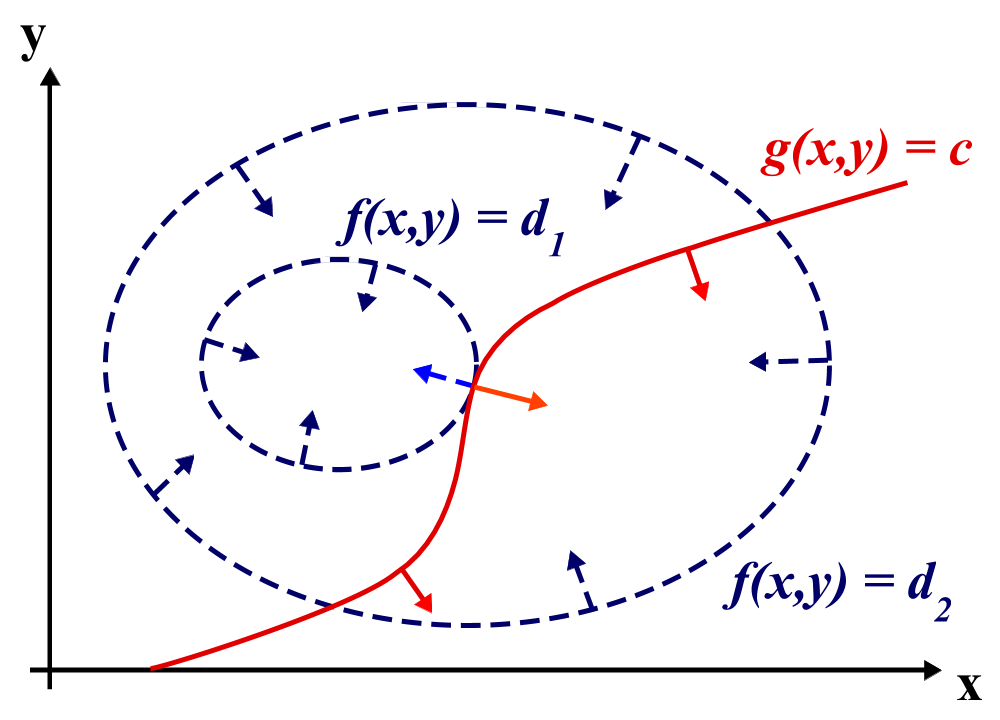
\includegraphics[width=0.5\linewidth]{lagrangian-optimization}
% \end{center}
% If the gradients were not parallel, we could move along $g(x,y)=c$ to a higher contour of $f(x,y)$ by following the component of $\nabla f$ parallel to $g(x,y)=c$.


% \newpage
% \section{Functional Derivatives}\label{app:functional-derivatives}

% A functional is just a function of a function -- i.e.\ some rule $F$ that maps a function $f$ into a number $F[f]$.  Definite integrals are a common example.
% In order to optimize a functional $F$ with respect to its argument $f$, one needs to take a \textit{functional derivative}.\footnote{\url{http://en.wikipedia.org/wiki/Functional_derivative}}
% To motivate the definition of a functional derivative, first consider the definition of an ordinary derivative
% \begin{align}
%   \fd{f(x)}{x}
% \equiv
%   \lim_{\e\rightarrow0}
%   \fr{f(x+\e)-f(x)}{\e}
% \end{align}
% and note the following identity, which you can verify using
% $
%   f(x+\e)
% =
%   f(x)
% +
%   \dfd{f(x)}{x}
%   \e
% +
%   \mc{O}(\e^2)
% $.
% \begin{align}\label{eq:scalar-derivative-trick}
%   \lim_{\e\rightarrow0}
%   \fr{f(x+\e)-f(x)}{\e}
% =&\
% \left.
%   \fr{df(x+\e)}{d\e}
% \right|_{\e=0}
% \end{align}
% For multivariate functions, we have the concept of a \textit{directional derivative}
% \begin{align}\label{eq:directional-derivative}
%   \bo{y}\cdot
%   \pd{f(\bo{x})}{\bo{x}}
% =
%   \lim_{\e\rightarrow0}
%   \fr{f(\bo{x}+\e\bo{y}) - f(\bo{x})}{\e}
% \end{align}
% which measures the change in $f(\bo{x})$ in the direction $\bo{y}$.
% Using equation \ref{eq:scalar-derivative-trick}, the directional derivative can be evaluated as an ordinary scalar derivative with respect to $\e$.
% \begin{align}\label{eq:vector-derivative-trick}
%   \bo{y}\cdot
%   \pd{f(\bo{x})}{\bo{x}}
% =
%   \left.
%   \fd{f(\bo{x} + \e\bo{y})}{\e}
%   \right|_{\e=0}
% \end{align}
% The functional derivative $\dfr{\d F}{\d f}$ is defined to satisfy an equation analogous to \ref{eq:directional-derivative}, playing the role of the gradient.
% \begin{align}
%   \int_{-\infty}^{\infty}
%   dx'\,
%   g(x')
%   \fr{\d F[f]}{\d f(x')}
% \equiv
%   \lim_{\e\rightarrow0}
%   \fr{F[f+\e g] - F[f]}{\e}
% \end{align}
% This left-hand side could be called a \textit{functional directional derivative}, giving the change in $F$ upon displacing its argument along the function $g$.
% Here, the integral takes the role of the dot product in \ref{eq:directional-derivative}.
% Using the same trick as in equation \ref{eq:vector-derivative-trick}, the functional derivative can be expressed as an ordinary scalar derivative.
% \begin{align}
% \label{eq:functional-derivative-trick}
%   \int_{-\infty}^{\infty}
%   dx'\,
%   g(x')
%   \fr{\d F[f]}{\d f(x')}
% =
%   \left.
%   \fd{F[f+\e g]}{\e}
%   \right|_{\e=0}
% \end{align}
% The standard procedure for evaluating the functional derivative is to first evaluate the right-hand side of equation~\ref{eq:functional-derivative-trick} for an arbitrary $g$ and then infer what $\dfr{\d F[f]}{\d f(x)}$ must be by comparing to the left-hand side.
% Equivalently, $g(x')$ can be replaced with a Dirac delta $\d(x-x')$ in order to arrive at $\dfr{\d F[f]}{\d f(x)}$ directly.

% Using eq. \ref{eq:functional-derivative-trick} and the lemma in \cref{app:fundamental-lemma-of-calculus-of-variations}, we find that the stationarity condition for a functional
% \begin{align}
%   \fr{\d F[f]}{\d f}
% \overset{!}{=}
%   0
% \end{align}
% is equivalent to the following condition.
% \begin{align}
%   \left.
%   \fd{F[f+\e g]}{\e}
%   \right|_{\e=0}
% \overset{!}{=}
%   0
% &&
%   \text{for all $g(x)$}
% \end{align}


% \newpage
% \section{Fundamental Lemma of Calculus of Variations}\label{app:fundamental-lemma-of-calculus-of-variations}
% The \textit{Fundamental Lemma of Calculus of Variations}\footnote{\url{http://en.wikipedia.org/wiki/Fundamental_lemma_of_calculus_of_variations}} says that, for continuous functions, the condition
% \begin{align}
%   \int_{-\infty}^\infty dx f(x)\eta(x)
% =
%   0
% \text{ for all $\eta(x)$}
% \end{align}
% holds only when $f(x)=0$ for all $x$.
% We can see this by considering the case $\eta(x)=f(x)$.
% Since $f(x)^2$ is nonnegative everywhere, the integral yields a positive number whenever $f(x)\neq 0$ on a finite range of $x$ values.



% \newpage
% \section{Unitary Invariances for Hartree-Fock Orbitals}\label{app:hartree-fock-orbital-invariance}

% \paragraph{Orthonormality.}
% By definition, unitary transformations preserve overlaps.
% This can be verified as follows
% \begin{align*}
%   \ip{\tl\y_i|\tl\y_j}
% =
% \sum_{kl}
%   U_{ki}U_{lj}^*
%   \ip{\y_k|\y_l}
% =
% \sum_{kl}
%   U_{ki}U_{lj}^*
%   \d_{kl}
% =
% \sum_k
%   U_{ki}U_{kj}^*
% =
%   \d_{ij}
% \end{align*}
% %using $\sum_k U_{ki}U_{kj}^*=(\bo{U}\bo{U}\dg)_{ji}=(\bo{1})_{ji}=\d_{ji}$.

% \paragraph{Fock operator.}
% Only the Coulomb and exchange parts of the Fock operator depend on the orbital set.
% For the Coulomb part, we have
% {\small\begin{align*}
% \sum_i
%   \ip{\tl\y_i(2)|\op{g}(1,2)|\tl\y_i(2)}
% =
% \sum_{ijk}
%   U_{ji}U_{ki}^*
%   \ip{\y_j(2)|\op{g}(1,2)|\y_k(2)}
% =
% \sum_{jk}
%   \d_{jk}
%   \ip{\y_j(2)|\op{g}(1,2)|\y_k(2)}
% =
% \sum_j
%   \ip{\y_j(2)|\op{g}(1,2)|\y_j(2)}
% \end{align*} \underline{}}%
% using the fact that $\sum_i U_{ji}U_{ki}^*=\d_{jk}$.
% For the exchange part, we have the same thing with a $\op{P}(1,2)$ sandwiched in there.

% \paragraph{Hamiltonian expectation value.}
% The vector notation $\bm\y$ for our orbitals allows us to express $\F$ and $\tl\F$ as
% \begin{align*}
%   \F(1,\ld,n)
% =
%   \tfrac{1}{\sqrt{n!}}
%   |\bm\y(1)\cd\bm\y(n)|
% %\sp\sp
%   \tl\F(1,\ld,n)
% =
%   \tfrac{1}{\sqrt{n!}}
%   |\tl{\bm\y}(1)\cd\tl{\bm\y}(n)|
% \end{align*}
% which, noting that the matrix $\ma{\tl{\bm\y}(1)\ \cd\ \tl{\bm\y}(n)}$ is simply
% \begin{align*}
%   \ma{\tl{\bm\y}(1)\ \cd\ \tl{\bm\y}(n)}
% =
%   \ma{\bo{U}\dg\bm\y(1)\ \cd\ \bo{U}\dg\bm\y(n)}
% =
%   \bo{U}\dg\ma{\bm\y(1)\ \cd\ \bm\y(n)}
% \end{align*}
% implies $\tl\F=\det(\bo{U}\dg)\F=\det(\bo{U})^*\F$.
% Therefore, $\tl{\F}$ and $\F$ have the same energy expectation values.
% \begin{align}
%   \ip{\tl\F|\op{H}_e|\tl\F}
% =
%   \det(\bo{U}\bo{U}\dg)\ip{\F|\op{H}_e|\F}
% =
%   \ip{\F|\op{H}_e|\F}
% \end{align}

\chapter{The Roothaan-Hall and Pople-Nesbet equations}

\section{Spin and spin-orbitals}

A spin-orbital $\y$ can be expressed as $\y(\bo{r},s)=\f(\bo{r})\w(s)$, where $\f(\bo{r})$ is a spatial orbital and $\w(s)$ is a spin function.
Spin functions live in a two-dimensional space spanned by $\{\alpha(s),\beta(s)\}$, which are orthonormal eigenfunctions of one component of $\op{\bo{S}}$, the spin angular momentum operator.
\begin{align}
  \op{S}_z\alpha
=
  +\fr{1}{2}\alpha
&&
  \op{S}_z\beta
=
  -\fr{1}{2}\beta
&&
  \ip{\alpha|\alpha}=\ip{\beta|\beta}=1
&&
  \ip{\alpha|\beta}=\ip{\beta|\alpha}=0
\end{align}
The ``spin-coordinate'' $s$ is either $+$ or $-$, identifying the component of $\w(s)$ along $\a(s)$ and $\b(s)$.
You can think of it as the index of a coordinate vector in spin space
\begin{align*}
  \ma{\w(+)\\\w(-)}
=
  \ma{\ip{\alpha|\w}\\\ip{\beta|\w}}
\end{align*}
so that $\alpha(+)=\beta(-)=1$ and $\a(-)=\beta(+)=0$.
Using this spin coordinate, the inner product in spin space can be defined explicitly as $\ip{\w|\w'}=\sum_s\w^*(s)\w'(s)$.
This is commonly referred to as a ``spin integration'', even though it looks more like a dot product.

A complete set of one-electron functions (spin-orbitals) comes in $\a,\b$-pairs.
\begin{align}\label{eq:spin-orb-general}
	\y_{2p-1}(\bo{r},s)
=
  \f_{p_\alpha}(\bo{r})\alpha(s)
&&
  \y_{2p}(\bo{r},s)
=
  \f_{p_\beta}(\bo{r})\beta(s)
\end{align}
The spatial components of these functions can be expanded in terms of a set of AO basis functions $\{\x_\nu\}$ as
\begin{align}\label{eq:space-orb}
  \f_{p_\alpha}
=
  \sum_\mu \x_\mu C_{\mu p_\alpha}
&&
  \f_{p_\beta}
=
  \sum_\mu \x_\mu C_{\mu p_\beta}
\end{align}
where the AOs basis set consists of atom-centered Gaussian functions (cc-pVTZ, 6-31G, etc.).



% \section{Spin-integration of the canonical Hartree-Fock equations}

% For a system with $n_\alpha$ spin-up and $n_\beta$ spin-down electrons, the spin-orbital canonical Hartree-Fock equation takes the following form.
% \begin{align}\label{eq:canonical-hf}
% &
%   \op{f}\y_p
% =
%   \ev_p\y_p
% &&
%   \op{f}
% =
%   \op{h}
% +
%   \sum_{i_\alpha}^{n_\alpha}
%   (\op{J}_{i_\alpha}-\op{K}_{i_\alpha})
% +
%   \sum_{i_\beta}^{n_\beta}
%   (\op{J}_{i_\beta}-\op{K}_{i_\beta})
% \end{align}
% This equation can be expanded in the spin basis as
% \begin{align}
%   \ma{
%     \ip{\a|\op{f}|\a}&\ip{\a|\op{f}|\b}\\
%     \ip{\b|\op{f}|\a}&\ip{\b|\op{f}|\b}}
%   \ma{
%     \ip{\a|\y_p}\\
%     \ip{\b|\y_p}}
% =
%   \ev_p
%   \ma{
%     \ip{\a|\y_p}\\
%     \ip{\b|\y_p}}
% \end{align}
% where we are integrating over the spin coordinate.
% The operators in $\op{f}$ then become
% \begin{align}
% &
%   \op{h}
% \mapsto
%   \ma{
%     \ip{\a|\op{h}|\a}&0\\
%     0&\ip{\b|\op{h}|\b}}
% &&
% \begin{array}{r@{\ }l@{\hspace{1cm}}r@{\ }l}
%   \op{J}_{i_\a}
% &\mapsto
%   \ma{
%     \ip{\a|\op{J}_{i_\a}|\a}&0\\
%     0&\ip{\b|\op{J}_{i_\a}|\b}}
% &
%   \op{K}_{i_\a}
% &\mapsto
%   \ma{
%     \ip{\a|\op{K}_{i_\a}|\a}&0\\
%     0&\makebox[\widthof{\ip{\b|\op{K}_{i_\b}|\b}}]{0}}
% \\[10pt]
%   \op{J}_{i_\b}
% &\mapsto
%   \ma{
%     \ip{\a|\op{J}_{i_\b}|\a}&0\\
%     0&\ip{\b|\op{J}_{i_\b}|\b}}
% &
%   \op{K}_{i_\b}
% &\mapsto
%   \ma{
%     \makebox[\widthof{\ip{\a|\op{K}_{i_\a}|\a}}]{0}&0\\
%     0&\ip{\b|\op{K}_{i_\b}|\b}}
% \end{array}
% \end{align}
% where the core and Coulomb operators can be evaluated as $\ip{\w|\op{h}|\w'}=\op{h}\ip{\w|\w'}$, since they don't act on spin coordinates.
% The exchange operator, however, does act on spin coordinates by its coordinate-swapping operation.
% \begin{align}
%   \op{K}_{i_\a}(\bo{r})\a(s)
% =&\
%   \sum_{s'}
%   \ip{\f_{i_\a}(\bo{r}')\a(s')|\op{g}(\bo{r},\bo{r}')|\cdot(\bo{r}')\a(s')}\,
%   \f_{i_\a}(\bo{r})\a(s)
% =
%   \ip{\f_{i_\a}(\bo{r}')|\op{g}(\bo{r},\bo{r}')|\cdot(\bo{r}')}\,
%   \f_{i_\a}(\bo{r})\a(s)
% \\
%   \op{K}_{i_\b}(\bo{r})\a(s)
% =&\
%   \sum_{s'}
%   \ip{\f_{i_\b}(\bo{r}')\b(s')|\op{g}(\bo{r},\bo{r}')|\cdot(\bo{r}')\a(s')}\,
%   \f_{i_\b}(\bo{r})\b(s)
% =
%   0
% \end{align}
% Here, the $\cdot$ means ``fill in spatial function here'' and the matrix elements are integrated over $\bo{r}'$.
% This shows why $\ip{\a|\op{K}_{i_\b}|\a}=\ip{\b|\op{K}_{i_\b}|\a}=\ip{\b|\op{K}_{i_\a}|\a}=0$ and $\ip{\a|\op{K}_{i_\a}|\a}\neq0$.
% The remaining components can be derived in the same way.

% Since all of the off-diagonal elements in the spin basis vanish, we can separate \cref{eq:canonical-hf} into two equations.
% \begin{align}\label{eq:canonical-uhf-equation-alpha}
% &
%   \op{f}_\alpha \f_{p_\alpha}
% =
%   \ev_{p_\alpha} \f_{p_\alpha}
% &&
%   \op{f}_\alpha
% =
%   \op{h}
% +
%   \sum_{i_\alpha}^{n_\alpha}
%   (\op{J}_{i_\alpha} - \op{K}_{i_\alpha})
% +
%   \sum_{i_\beta}^{n_\beta}
%   \op{J}_{i_\beta}
% \\\label{eq:canonical-uhf-equation-beta}
% &
%   \op{f}_\beta \f_{p_\beta}
% =
%   \ev_{p_\beta} \f_{p_\beta}
% &&
%   \op{f}_\beta
% =
%   \op{h}
% +
%   \sum_{i_\alpha}^{n_\alpha}
%   \op{J}_{i_\alpha}
% +
%   \sum_{i_\beta}^{n_\beta}
%   (\op{J}_{i_\beta} - \op{K}_{i_\beta})
% \end{align}




% \section{RHF: The Roothaan-Hall Equations}

% Assuming a closed-shell system with $n_\a=n_\b=n/2$, we can impose the restriction that $\f_{i_\a}=\f_{i_\b}$ for each pair of electrons.
% Then equations~\ref{eq:canonical-uhf-equation-alpha} and~\ref{eq:canonical-uhf-equation-beta} collapse into a single expression.
% \begin{align*}
%   \op{f}_\textsc{r}\f_p
% =
%   \ev_p\f_p
% &&
%   \op{f}_\textsc{r}
% =
%   \op{h}
% +
%   \sum_i^{n/2}
%   (2\op{J}_i - \op{K}_i)
% \end{align*}
% where the R stands for ``restricted''.
% Expanding $\f_p$ in the AO basis and projecting by $\x_\mu$, we get
% \begin{align*}
%   \sum_\nu
%   \ip{\x_\mu|\op{f}_\textsc{r}|\x_\nu}
%   C_{\nu p}
% =
%   \sum_\nu
%   \ip{\x_\mu|\x_\nu}C_{\mu p}\ev_p
% \end{align*}
% which are the \textit{Roothaan-Hall equations}.
% In matrix notation, these can be written as follows.
% \begin{align}\label{eq:roothaan-hall}
% &
%   \bo{F}\bo{C}
% =
%   \bo{S}\bo{C}\bm{\ev}
% &&
%   F_{\mu\nu}
% =
%   \ip{\x_\mu|\op{f}_\textsc{r}|\x_\nu}
% &&
%   S_{\mu\nu}
% =
%   \ip{\x_\mu|\x_\nu}
% &&
%   (\bm{\ev})_{pq}
% =
%   \ev_p\d_{pq}
% \end{align}
% Note that if the AO basis contains $m$ functions, then $\bo{C}=[C_{\mu p}]$ is an $m\times m$ matrix with each column vector containing the expansion coefficients for an orbital $\f_p$.
% Also, note that only the $n/2$ MOs of lowest energy ($\ev_p$) will be ``occupied'' -- the remaining virtual orbitals will not enter into the Coulomb and exchange parts of $\op{f}_\textsc{R}$.
% Expanding $\op{f}_\textsc{R}$ in its core, Coulomb, and exchange parts, we find
% \begin{align*}
%   F_{\mu\nu}
% =&\
%   \ip{\x_\mu|\op{h}|\x_\nu}
% +
%   \sum_i^{n/2}
%   (2\ip{\x_\mu\f_i|\x_\nu\f_i}-\ip{\x_\mu\f_i|\f_i\x_\nu})
% \\
% =&\
%   \ip{\x_\mu|\op{h}|\x_\nu}
% +
%   \sum_i^{n/2}
%   \sum_{\rho\si}^m
%   C_{\rho i}^*C_{\si i}
%   (2\ip{\x_\mu\x_\rho|\x_\nu\x_\si}-\ip{\x_\mu\x_\rho|\x_\si\x_\nu})
% \end{align*}
% which is conveniently given in terms of a ``density matrix'' $D_{\mu\nu}$.
% \begin{align}\label{eq:rhf-ao-basis-fock}
%   F_{\mu\nu}
% =&\
%   \ip{\x_\mu|\op{h}|\x_\nu}
% +
%   \sum_{\rho\si}^m
%   D_{\rho\si}
%   (2\ip{\x_\mu\x_\rho|\x_\nu\x_\si}-\ip{\x_\mu\x_\rho|\x_\si\x_\nu})
% &&
%   D_{\mu\nu}
% =
%   \sum_i^{n/2}
%   C_{\mu i}^*C_{\nu i}
% \end{align}




% \subsection{Solving the Roothaan-Hall Equations}

% Equation~\ref{eq:roothaan-hall} would look like an ordinary eigenvalue problem if $\bo{S}$ were an identity matrix.
% This would be the case if the AO basis were orthogonal, but that generally isn't the case.
% We can get around this problem using the following algebraic trick:
% if we multiply both sides of equation~\ref{eq:roothaan-hall} by $\bo{S}^{-\frac{1}{2}}$ and insert $\bo{I}=\bo{S}^{-\frac{1}{2}}\bo{S}^{\frac{1}{2}}$ between $\bo{F}$ and $\bo{C}$, we can write
% \begin{align}
% \label{orthogonalized-roothaan-hall}
% &
%   \tl{\bo{F}}
%   \tl{\bo{C}}
% =
%   \tl{\bo{C}}\bm\ev
% &&
%   \tl{\bo{F}}
% =
%   \bo{S}^{-\frac{1}{2}}\bo{F}\bo{S}^{-\frac{1}{2}}
% &&
%   \tl{\bo{C}}
% =
%   \bo{S}^{\frac{1}{2}}\bo{C}\ .
% \end{align}
% This is equivalent to a transformation to an orthogonalized AO basis $\tl\x_\mu=\sum_\nu\x_\nu (\bo{S}^{-\frac{1}{2}})_{\nu\mu}$ which satisfies $\ip{\tl\x_\mu|\tl\x_\nu}=\d_{\mu\nu}$.
% After diagonalizing the transformed Fock matrix, $\tl{\bo{F}}$, the MO coefficients with respect to the original non-orthogonal AO basis can be recovered as $\bo{C}=\bo{S}^{-\frac{1}{2}}\tl{\bo{C}}$.

% \begin{samepage}
% Equation~\ref{orthogonalized-roothaan-hall} is still not exactly an ordinary eigenvalue problem because $\bo{F}$ depends on the MOs via the density matrix $\bo{D}$.
% The standard procedure for solving the Roothaan-Hall equations repeatedly diagonalizes $\tl{\bo{F}}$ and feeds in the new density until the equation becomes self-consistent.
% The algorithm looks as follows.
% \begin{enumerate}
%   \item Get integrals $\ip{\x_\mu|\x_\nu}, \ip{\x_\mu|\op{h}|\x_\nu}, \ip{\x_\mu\x_\nu|\x_\rho\x_\si}$ and form orthogonalizer $\bo{S}^{-\frac{1}{2}}$
%   \item Guess $\bo{D}=\bo{0}$
%   \item\label{loop} Build $\bo{F}$ (equation~\ref{eq:rhf-ao-basis-fock})
%   \item Diagonalize $\tl{\bo{F}}=\bo{S}^{-\frac{1}{2}}\bo{F}\bo{S}^{-\frac{1}{2}}$ to get $\tl{\bo{C}}$ and $\bm\ev$
%   \item Backtransform to original basis: $\bo{C}=\bo{S}^{-\frac{1}{2}}\tl{\bo{C}}$
%   \item Form new density matrix: $D_{\mu\nu}=\sum_i^{n/2} C_{\mu i}^*C_{\nu i}$
%   \item If the new $\bo{D}$ differs from the old $\bo{D}$ by more than some threshold, return to step~\ref{loop}
% \end{enumerate}
% \end{samepage}


% \section{UHF: The Pople-Nesbet Equations}

% For open-shell systems of arbitrary $n_\a, n_\b$, we can solve equations~\ref{eq:canonical-uhf-equation-alpha} and~\ref{eq:canonical-uhf-equation-beta} without requiring $\f_{i_\a}=\f_{i_\b}$.
% By exactly the same procedure as was used for the Roothaan-Hall equations, this leads to \textit{Pople-Nesbet equations}
% \begin{align*}
% &
%   \bo{F}^\a\bo{C}^\a
% =
%   \bo{S}\bo{C}^\a\bm\ev^\a
% &&
%   F_{\mu\nu}^\a
% =
%   \ip{\x_\mu|\op{f}_\a|\x_\nu}
% &&
%   S_{\mu\nu}
% =
%   \ip{\x_\mu|\x_\nu}
% &&
%   (\bm\ev^\a)_{p_\a q_\a}
% =
%   \ev_{p_\a}\d_{p_\a q_\a}
% \\
% &
%   \bo{F}^\b\bo{C}^\b
% =
%   \bo{S}\bo{C}^\b\bm\ev^\b
% &&
%   F_{\mu\nu}^\b
% =
%   \ip{\x_\mu|\op{f}_\b|\x_\nu}
% &&
%   S_{\mu\nu}
% =
%   \ip{\x_\mu|\x_\nu}
% &&
%   (\bm\ev^\b)_{p_\b q_\b}
% =
%   \ev_{p_\b}\d_{p_\b q_\b}
% \end{align*}
% where $\bo{C}^\a=[C_{\mu p_\a}]$ is an $m\times m$ matrix of MO coefficients for $\{\f_{p_\a}\}$ and $\bo{C}^\b=[C_{\mu p_\b}]$ is an $m\times m$ matrix of MO coefficients for $\{\f_{p_\b}\}$.
% Expanding the $\a$ and $\b$ Fock matrices as in equation~\ref{eq:rhf-ao-basis-fock}, we find
% \begin{align*}
% &
%   F_{\mu\nu}^\a
% =
%   \ip{\x_\mu|\op{h}|\x_\nu}
% +
%   \sum_{\rho\si}
%   D_{\rho\si}^\a
%   \ip{\x_\mu\x_\rho||\x_\nu\x_\si}
% +
%   \sum_{\rho\si}
%   D_{\rho\si}^\b
%   \ip{\x_\mu\x_\rho|\x_\nu\x_\si}
% &&
%   D_{\mu\nu}^\a
% =
%   \sum_{i_\a}^{n_\a} C_{\mu i_\a}^*C_{\nu i_\a}
% \\
% &
%   F_{\mu\nu}^\b
% =
%   \ip{\x_\mu|\op{h}|\x_\nu}
% +
%   \sum_{\rho\si}
%   D_{\rho\si}^\a
%   \ip{\x_\mu\x_\rho|\x_\nu\x_\si}
% +
%   \sum_{\rho\si}
%   D_{\rho\si}^\b
%   \ip{\x_\mu\x_\rho||\x_\nu\x_\si}
% &&
%   D_{\mu\nu}^\b
% =
%   \sum_{i_\b}^{n_\b} C_{\mu i_\b}^*C_{\nu i_\b}
% \end{align*}
% where $\bo{D}^\a$ and $\bo{D}^\b$ are the $\a$ and $\b$ density matrices.
% The procedure for solving the Pople-Nesbet equations is identical to the one given for RHF\@.
% However, note that one must solve the $\a$ and $\b$ equations simultaneously because each Fock operator depends on both $\bo{C}^\a$ and $\bo{C}^\b$ (via $\bo{D}^\a$ and $\bo{D}^\b$).

\chapter{Second Quantization}

\minitoc

\begin{dfn}\label{dfn:slater-determinant}
\thmtitle{Slater determinant}
A \textit{Slater determinant} is a normalized antisymmetric product of spin-orbitals
\begin{align}\label{eq:slater-determinant-position-representation}
  \F_{(p_1\cd p_n)}(1,\ld,n)
=
  \tfr{1}{\sqrt{n!}}
  \sum_{\pi}^{\mr{S}_n}
  \e_{\pi}
  \y_{p_{\pi(1)}}(1)\cd\y_{p_{\pi(n)}}(n)
\end{align}
where $\pi\in\mr{S}_n$ is a permutation of $(1,\cd, n)$ with signature $\e_{\pi}$.\footnote{The signature of a permutation is $(-)^{\text{\# transpositions}}$.  See \url{https://en.wikipedia.org/wiki/Symmetric_group} for more on $\mr{S}_n$.}
\end{dfn}

\section{Deriving the second-quantized Hamiltonian from first quantization}\label{ssec:direct-derivation-of-second-quantization}

Let $\mc{F}_n$ denote the span of $n$-electron determinants and consider the integral operator $\op{a}_p:\mc{F}_n\rightarrow \mc{F}_{n-1}$ given by
\begin{align}
  (\op{a}_p\Y)(2,\cd,n)
\equiv
  \sqrt{n}\int d(1) \y_p^*(1)\Y(1,2,\cd,n)\,.
\end{align}
This operator acts on Slater determinants as follows.
\begin{align}
  (\op{a}_p\F_{(p_1\cd p_n)})(2,\cd,n)
=
\left\{
\ar{
  (-)^{k-1}\F_{(p_1\cd \cancel{p_k}\cd p_n)}(2,\ld,n) & p=p_k\in(p_1\cd p_n)\\[5pt]
  0 & \text{otherwise}
}
\right.
\end{align}
In words, it deletes $\y_p$ from $\F_{(p_1\cd p_n)}$ if present, otherwise killing the determinant.
The restriction to an antisymmetric space makes these operators anticommute, $\op{a}_p\op{a}_q=-\op{a}_q\op{a}_p$, since it can be shown that for $\Y\in\mc{F}_n$
\begin{align*}
  \int d(1)d(2)\y_p^*(1)\y_q^*(2)\Y(1,2,\cd,n)
=&\
-
  \int d(1)d(2)\y_q^*(1)\y_p^*(2)\Y(1,2,\cd,n)
\end{align*}
by swapping integration variables.
These operators can be used to generate the following decompositions.\footnote{These follow from substituting in the definition of $\op{a}_p$ and applying resolution of the identity to each argument.}
\begin{align}
  \Y(1,\cd,n)
=&\
  \tfr{1}{\sqrt{n}}
  \sum_p^\infty\y_p(1)\pr{\op{a}_p\Y}(2,\cd,n)
\\=&\
  \tfr{1}{\sqrt{n(n-1)}}
  \sum_{pq}^\infty
  \y_p(1)\y_q(2)(\op{a}_q\op{a}_p\Y)(3,\cd,n)
\end{align}
Therefore, matrix elements of the electronic Hamiltonian with respect to $\Y,\Y'\in \mc{F}_n$ can be expressed as
\begin{align*}
  \ip{\Y|\op{H}\Y'}
=
  \sum_{i=1}^n\ip{\Y|\op{h}(i)\Y'}
+
  \sum_{i<j}^n\ip{\Y|\op{g}(i,j)\Y'}
=&\
  n\ip{\Y|\op{h}(1)\Y'}
+
  \tfr{n(n-1)}{2}
  \ip{\Y|\op{g}(1,2)\Y'}
\\=&\
  \sum_{pq}^\infty
  h_{pq}\ip{\op{a}_p\Y|\op{a}_q\Y'}
+
  \tfr{1}{2}
  \sum_{pqrs}^\infty
  \ip{pq|rs}\ip{\op{a}_q\op{a}_p\Y|\op{a}_s\op{a}_r\Y'}
\end{align*}
in terms of the usual one- and two-electron integrals.
Since $\Y$ and $\Y'$ are arbitrary elements of $\mc{F}_n$, this implies
\begin{align}\label{eq:second-quantized-hamiltonian}
  \left.
  \op{H}
  \right|_{\mc{F}_n}
=
  \sum_{pq}^\infty
  h_{pq}
  \op{a}_p\dg \op{a}_q
+
  \tfr{1}{2}
  \sum_{pqrs}^\infty
  \ip{pq|rs}
  \op{a}_p\dg\op{a}_q\dg\op{a}_s\op{a}_r
\end{align}
which is the \textit{second quantized} form of the Hamiltonian, as opposed to the \textit{first quantized} form which is not restricted to antisymmetric functions.
A defining feature of the second quantization formalism is that $\op{H}$ is independent of the number of electrons, because \cref{eq:second-quantized-hamiltonian} holds for all $n$.

\section{Formal treatment of second quantization}

\begin{dfn}\label{dfn:direct-sum-and-direct-product}
\thmtitle{Direct sums and products}
\begin{samepage}
The \textit{direct sum}, $\oplus$, and \textit{direct product}\footnote{Also known as a \textit{tensor product}}, $\otimes$, are operations defining two different ways of combining vector spaces.
Each operation takes a vector from one space and a vector the other to form an ordered pair, but they behave differently under vector addition and scalar multiplication.
In a direct sum space $V\oplus V'\equiv\{v\oplus v'\,|\,v\in V,\,v'\in V'\}$,
vector addition and scalar multiplication are defined by
\begin{align}
  v_1\oplus v_1'
+
  v_2\oplus v_2'
=
  (v_1 + v_2)
\oplus
  (v_1' + v_2')
&&
  c(v\oplus v')
=
  cv\oplus cv'\,,
\end{align}
whereas, in a direct product space $V\otimes V'\equiv\{\sum v\otimes v'\,|\,v\in V,\,v'\in V'\}$, they are defined as follows.
\begin{align}
  v_1\otimes v'
+
  v_2\otimes v'
=
  (v_1 + v_2)\otimes v'
&&
  v\otimes v_1'
+
  v\otimes v_2'
=
  v\otimes(v_1' + v_2')
&&
  c(v\otimes v')
=
  (cv)\otimes v'
=
  v\otimes(cv')
\end{align}
Note that $\oplus$ behaves like addition and $\otimes$ behaves like multiplication.
If $\{e_i\}$ and $\{e_{i'}'\}$ are basis sets for $V$ and $V'$, respectively, then $\{e_i\oplus0'\}\cup\{0\oplus e_{i'}'\}$ is a basis for their direct sum and $\{e_i\otimes e_{i'}'\}$ is a basis for their direct product.
The dimension of the direct sum space is the sum of their dimensions,
$\dim V+\dim V'$,
and that of the direct product space is the product of their dimensions,
$\dim V\cdot \,\dim V'$.
Finally, if $\ip{\cdot|\cdot}_V$ and $\ip{\cdot|\cdot}_{V'}$ are inner products on $V$ and $V'$, then the following are inner products on the combined spaces.
\begin{align}
  \ip{v\oplus v'|w\oplus w'}_{V\oplus V'}
\equiv
  \ip{v|w}_V
+
  \ip{v'|w'}_{V'}
&&
  \ip{v\otimes v'|w\otimes w'}_{V\otimes V'}
\equiv
  \ip{v|w}_V
\cdot
  \ip{v'|w'}_{V'}
\end{align}
\end{samepage}
\end{dfn}


\begin{dfn}
\thmtitle{Hilbert space}
If $\mc{H}$ is a one-electron Hilbert space spanned by a set of spin-orbitals $\{\y_p\}$, then $\mc{H}^{\otimes n}=\mc{H}\otimes\cd\otimes\mc{H}=\spn\{\y_{p_1}{}\otimes\cd\otimes\y_{p_n}\}$ is an \textit{$n$-electron Hilbert space}.\footnote{These basis vectors are abstract representations spin-orbital product functions, $\ip{1\otimes\cd\otimes n|\y_{p_1}\otimes\cd\otimes\y_{p_n}}=\y_{p_1}(1)\cd\y_{p_n}(n)$, which are known as \textit{Hartree products}.}
\end{dfn}


\begin{dfn}\label{dfn:fock-space}
\thmtitle{Fock space}
Let $\mc{F}_n(\mc{H})$ denote $\spn\{\F_{(p_1\cd p_n)}\}$,\footnote{%
These basis vectors are Slater determinants, abstracted from position space:
$
  \F_{(p_1\cd p_n)}
=
  \fr{1}{\sqrt{n!}}
  \sum_{\pi\in\mr{S}_n}
  \y_{p_{\pi(1)}}\otimes\cd\otimes
  \y_{p_{\pi(n)}}
$.
Equation~\ref{eq:slater-determinant-position-representation} corresponds to
$
  \ip{1\otimes\cd\otimes n|\F_{(p_1\cd p_n)}}= \F_{(p_1\cd p_n)}(1,\ld,n)
$.
}
the antisymmetric subspace of $\mc{H}^{\otimes n}$.
\textit{Fock space} is the union of these spaces, $\mc{F}(\mc{H})=\mc{F}_0(\mc{H})\oplus \mc{F}_1(\mc{H})\oplus \mc{F}_2(\mc{H})\oplus\cd\oplus \mc{F}_{\infty}(\mc{H})$, comprising all possible electronic wavefunctions.
\end{dfn}

\begin{dfn}\label{occupation-number-representation}
\thmtitle{Occupation vectors}
In the \textit{occupation number formalism}, Fock space basis states are represented as \textit{occupation vectors}.
These are denoted by a series of bits,
$
  \kt{\bo{n}}
\equiv
  \kt{n_1,n_2,n_3,\cd,n_\infty}
$,
where $n_p=1$ when $\y_p$ is occupied and $n_p=0$ when it isn't.
The fully unoccupied state is called the \textit{vacuum}, denoted $\kt{\vac}$, which spans $\mc{F}_0(\mc{H})$.
\end{dfn}

\begin{dfn}\label{dfn:particle-hole-operators}
\thmtitle{Particle-hole operators}
\textit{Particle-hole operators} change the occupation numbers of one-particle states.
The \textit{annihilation operator} of $\y_p$ is a linear mapping $a_p:\mc{F}_n(\mc{H})\rightarrow \mc{F}_{n-1}(\mc{H})$ defined by
\begin{align}\label{eq:occ-num-annihilation-operator-action}
  a_p\kt{\cd n_p\cd}
=
  (-)^{n_1+\cd+n_{p-1}}
  \kt{\cd n_p-1\cd}
\ \ \ \text{if $n_p=1$}
&&
  a_p\kt{\cd n_p\cd}
=
  0
\ \ \ \text{if $n_p=0$}
\end{align}
and the \textit{creation operator} of $\y_p$ is a linear mapping $c_p:\mc{F}_n(\mc{H})\rightarrow \mc{F}_{n+1}(\mc{H})$ defined by
\begin{align}\label{eq:occ-num-creation-operator-action}
  c_p\kt{\cd n_p\cd}
=
  (-)^{n_1+\cd+n_{p-1}}
  \kt{\cd n_p+1\cd}
\ \ \ \text{if $n_p=0$\ }
&&
  c_p\kt{\cd n_p\cd}
=
  0
\ \ \ \text{if $n_p=1$.}
\end{align}
\end{dfn}

\begin{prop}
\thmtitle{$c_p=a_p\dg$}
\thmstatement{Creation and annihilation operators of the same state $\y_p$ are adjoints of each other.}
\thmproof{
  $\ip{n_1'n_2'\cd|a_p[n_1n_2\cd]}$ vanishes unless $n_p'=0$, $n_p=1$, and $n_q'=n_q\ \forall q\neq p$.
  Likewise for $\ip{c_p[n_1'n_2'\cd]|n_1n_2\cd}$.
  Therefore, $\ip{\Y|a_p\Y'}=\ip{c_p\Y|\Y'}$ for all $\Y,\Y'\in \mc{F}(\mc{H})$ and $c_p=a_p\dg$ by the definition of adjoint.
}
\end{prop}

\begin{prop}\label{prop:particle-hole-operator-anticommutator}
\thmtitle{$[q,q']_+=\delta_{q'q\dg}$}
\thmstatement{Particle-hole operators $q$ and $q'$ anticommute unless $q'=q\dg$, for which $[q,q\dg]_+=1$.}~\footnote{These are anticommutator brackets, $[q, q']_+ \equiv qq' + q'q$.}
\thmproof{
  Let $q$ and $q'$ be arbitrary particle-hole operators acting on $\y_p$ and $\y_{p'}$, respectively.
  First, suppose $p\neq p'$. Then
  \begin{align*}
  &
    qq'\kt{\cd n_p\cd n_{p'}\cd}
  =
    (-)^{n_p+\sum_{r=p+1}^{p'}n_r}
    \kt{\cd\ol{n_p}\cd\ol{n_{p'}}\cd}
  \,\text{, and}
  \\
  &
    q'q\kt{\cd n_p\cd n_{p'}\cd}
  =
    (-)^{\ol{n_p}+\sum_{r=p+1}^{p'}n_r}
    \kt{\cd\ol{n_p}\cd\ol{n_{p'}}\cd}
  \end{align*}
  where $\ol{n_p}$ and $\ol{n_{p'}}$ are the occupations after applying $q$ and $q'$.
  Since $n_p$ and $\ol{n_p}$ differ by one, $qq'=-q'q$.
  The second case, $p=p'$, implies $q'\in\{q,q\dg\}$.
  If $q'=q$, then $qq'=-q'q=0$.
  If $q'=q\dg$, either $n_p=1\implies(a_p\dg a_p + a_pa_p\dg)\kt{\cd n_p\cd}=(1+0)\kt{\cd n_p\cd}$ or $n_p=0\implies(a_p\dg a_p + a_pa_p\dg)\kt{\cd n_p\cd}=(0+1)\kt{\cd n_p\cd}$.
  Either way, $q'=q\dg\implies(qq' + q'q)=1$.
}
\end{prop}

\begin{rmk}
\thmtitle{Relating the determinant and occupation number formalisms}
When $p_1<\cd<p_n$, $\F_{(p_1\cd p_n)}$ is equivalent to the occupation vector $\kt{\bo{n}_{(p_1\cd p_n)}}$ with ones at $p_1,\cd,p_n$.
Otherwise, this determinant is equivalent to $\e_{\pi}\kt{\bo{n}_{(p_1\cd p_n)}}$ for $\pi\in\mr{S}_n$ such that $p_{\pi(1)}<\cd<p_{\pi(n)}$.
The actions of $a_p$ and $a_p\dg$ on $\F_{(p_1\cd p_n)}$ are given by
\begin{align}\label{eq:abstract-annihilation-operator-action}
  a_p\F_{(p_1\cd p_n)}
=
  (-)^{k-1}\F_{(p_1\cd\cancel{p_k}\cd p_n)}
  \ \text{if $p=p_k\in(p_1\cd p_n)$}
&&
  a_p\F_{(p_1\cd p_n)}
=
  0
  \ \text{if $p\notin(p_1\cd p_n)$}
\\\label{eq:abstract-creation-operator-action}
  a_p\dg\F_{(p_1\cd p_n)}
=
  (-)^{k-1}\F_{(p_1\cd p_{k-1}pp_k\cd p_n)}
  \ \text{if $p\notin(p_1\cd p_n)$}
&&
  a_p\dg\F_{(p_1\cd p_n)}
=
  0
  \ \text{if $p\in(p_1\cd p_n)$}
\end{align}
which follows directly from \Cref{eq:occ-num-annihilation-operator-action,eq:occ-num-creation-operator-action} when $p_1<\cd<p_n$.
Other cases follow from the fact that any sign factors for permuting $(p_1\cd p_n)$ cancel on both sides of the equation, including the position of insertion or deletion, $p_k$, whose phase is tracked by $(-)^{k-1}$ on the right.
That is, both sides of the equation are antisymmetric to permutations of $(1\cd n)$.
Note that \Cref{eq:abstract-annihilation-operator-action} was also derived in \Cref{ssec:direct-derivation-of-second-quantization} using the position-space representation of $a_p$.
One advantage of the determinant basis is that, unlike occupation vectors, determinants translate directly into strings of creations operators
\begin{align}
  \kt{\F_{(p_1\cd p_n)}}
=
  a_{p_1}\dg\cd a_{p_n}\dg\kt{\vac}
\end{align}
without any phase ambiguity.
Together with the second quantized form of the electronic Hamiltonian, this boils much of the grunt work of electronic structure theory down to particle-hole operator algebra.
\end{rmk}

\begin{dfn}
\thmtitle{Excitation operators and excited determinants}
Operator strings of the form $a_{p_1}\dg\cd a_{p_m}\dg a_{q_m}\cd a_{q_1}$ are called \textit{excitation operators}.
For a given reference determinant $\F$, excited determinants can be constructed as
\begin{align}
  \F_{i_1\cd i_m}^{a_1\cd a_m}
=
  a_{a_1}\dg\cd a_{a_m}\dg a_{i_m}\cd a_{i_1}\F
=
  a_{a_1}\dg a_{i_1}\cd a_{a_m}\dg a_{i_m}\F
\end{align}
where $i_1,\cd,i_m$ are occupied and $a_1,\cd,a_m$ are virtual indices with respect to $\F$.
\end{dfn}

\begin{dfn}\label{dfn:particle-hole-isomorphism}
\thmtitle{Particle-hole isomorphism}
The \textit{particle-hole isomorphism} with respect to the reference determinant $\kt{\F}=\kt{\underset{\text{$n$ times}}{1\cd1}\,0\,0\cd}$ is a mapping $F(\mc{H})\rightarrow F(\mc{H})$ that inverts the bits occupied in $\F$:
\begin{align*}
  \kt{k_1\cd k_nk_{n+1}k_{n+2}\cd}
\mapsto
  \kt{\ol{k}_1\cd \ol{k}_nk_{n+1}k_{n+2}\cd}
  \text{where $\ol{k}_i=1-k_i$.}
\end{align*}
Physically, this corresponds to shift in perspective from the \textit{particle frame} to a \textit{quasiparticle frame}, where the first $n$ states are viewed as \textit{holes} rather than \textit{particles}.
This makes $\kt{\vac}\mapsto\kt{\underset{\text{$n$ times}}{\ol{1}\cd\ol{1}}\,0\,0\cd}$ a state of $n$ holes and no particles.  $\kt{\F}\mapsto\kt{\underset{\text{$n$ times}}{\ol{0}\cd\ol{0}}\,0\,0\cd}$ becomes the \textit{quasiparticle vacuum state}, in which all hole and particle states are unoccupied.
\end{dfn}

\begin{dfn}
\thmtitle{Quasiparticle creation and annihilation operators}
If we apply \Cref{dfn:particle-hole-operators} to the new quasiparticle Fock space, we end up with a new system of \textit{quasi-particle-hole operators} $\{b_p\}\cup\{b_p\dg\}$, related to the old set via
\begin{align}
&&
  a_i
\mapsto
  b_i\dg
&&
  a_i\dg
\mapsto
  b_i
&&
  a_a
\mapsto
  b_a
&&
  a_a\dg
\mapsto
  b_a\dg
\end{align}
where $i$ and $a$ are occupied and virtual indices with respect to the reference determinant $\F$.
$\{a_i\dg\}\cup\{a_a\}\mapsto\{b_p\}$ are therefore \textit{quasiparticle annihilation operators} and $\{a_i\}\cup\{a_a\dg\}\mapsto\{b_p\dg\}$ are \textit{quasiparticle creation operators}.
\end{dfn}

\begin{rmk}
The standard expression for the second-quantized Hamiltonian is
\begin{align}
  H
=
  \sum_{pq}
  h_{pq}\,
  a_p\dg a_q
+
  \tfr{1}{4}
  \sum_{pqrs}
  \ip{pq||rs}\,
  a_p\dg a_q\dg a_sa_r
\end{align}
where the summations run over the full set of spin-orbitals.
Note that this matches \Cref{eq:second-quantized-hamiltonian}, except that we have rearranged the second term to express it in terms of antisymmetrized integrals.
In terms of quasi-particle-hole operators,
\begin{align}
\nonumber
  H
=&\
  \sum_{ab}
  h_{ab}\,
  b_a\dg b_b
+
  \sum_{ai}
  h_{ai}\,
  b_a\dg b_i\dg
+
  \sum_{ia}
  h_{ia}\,
  b_i b_a
+
  \sum_{ij}
  h_{ij}
  b_i b_j\dg
\\\nonumber&\
+
  \tfr{1}{4}
  \sum_{abcd}
  \ip{ab||cd}\,
  b_a\dg b_b\dg b_d b_c
+
  \tfr{1}{2}
  \sum_{abci}
  \ip{ab||ci}\,
  b_a\dg b_b\dg b_i\dg b_c
+
  \tfr{1}{2}
  \sum_{aibc}
  \ip{ai||bc}\,
  b_a\dg b_i b_c b_b
+
  \tfr{1}{4}
  \sum_{abij}
  \ip{ab||ij}\,
  b_a\dg b_b\dg b_j\dg b_i\dg
+
  \sum_{aibj}
  \ip{ai||bj}\,
  b_a\dg b_i b_j\dg b_b
\\&\
+
  \tfr{1}{4}
  \sum_{ijab}
  \ip{ij||ab}\,
  b_i b_j b_b b_a
+
  \tfr{1}{2}
  \sum_{iajk}
  \ip{ia||jk}\,
  b_i b_a\dg b_k\dg b_j\dg
+
  \tfr{1}{2}
  \sum_{ijka}
  \ip{ij||ka}\,
  b_i b_j b_a b_k\dg
+
  \tfr{1}{4}
  \sum_{ijkl}
  \ip{ij||kl}\,
  b_i b_j b_l\dg b_k\dg
\end{align}
where we have split the full summations above into summations over occupied and virtual orbitals and grouped like terms.
\end{rmk}

\begin{dfn}
\thmtitle{Normal order}
A string $q_1\cd q_n$ of particle-hole operators is in \textit{normal order} when all of its creation operators sit to the left of its annihilation operators.
That is, when the string has the form $a_{p_1}\dg\cd a_{p_m}\dg a_{r_1}\cd a_{r_{m'}}$.
This guarantees that its vacuum expectation value vanishes, $\ip{\vac|q_1\cd q_n|\vac}=0$.
More generally, we say that $q_1\cd q_n$ is in \textit{$\F$-normal order} if it maps into a string of the form $b_{p_1}\dg\cd b_{p_m}\dg b_{r_1}\cd b_{r_{m'}}$ under particle-hole isomorphism referenced to $\F$, since this guarantees that
$\ip{\F|q_1\cd q_n|\F}=0$.
\end{dfn}

\begin{ex}
In second quantization, any operator string can be expanded as a linear combination of strings which are in normal order.
The expectation value of a string is always equal to the constant term in this expansion.
For example:
\begin{align*}
  a_p a_q\dg
=
-
  a_q\dg a_p
+
  \delta_{pq}
&\implies
  \ip{\vac|a_p a_q\dg|\vac}
=
  \delta_{pq}
\\
  a_p a_q a_s\dg a_r\dg
=
  a_r\dg a_s\dg a_q a_p
+
  \delta_{ps}
  a_r\dg a_q
-
  \delta_{pr}
  a_s\dg a_q
-
  \delta_{qs}
  a_r\dg a_p
+
  \delta_{qr}
  a_s\dg a_p
-
  \delta_{ps}\delta_{qr}
+
  \delta_{pr}\delta_{qs}
&\implies
  \ip{\vac|a_p a_q a_s\dg a_r\dg|\vac}
=
  \delta_{pr}\delta_{qs}
-
  \delta_{ps}\delta_{qr}
\end{align*}
where we have made repeated use of \Cref{prop:particle-hole-operator-anticommutator} to arrive at these expansions.
This strategy becomes unwieldy for expectation values of a reference determinant $\F$, in which case it is more convenient to use particle-hole isomorphism.
For example, consider the following matrix element of the core Hamiltonian.
\begin{align*}
  \sum_{pq}
  h_{pq}
  \ip{\F|a_p\dg a_q|\F_i^a}
=
  \sum_{bc}
  h_{bc}\,
  \cancel{\ip{\F|b_b\dg b_c b_a\dg b_i\dg|\F}}
+
  \sum_{bj}
  h_{bj}\,
  \cancel{\ip{\F|b_b\dg b_j\dg b_a\dg b_i\dg|\F}}
+
  \sum_{jb}
  h_{jb}\,
  \cancelto{\d_{ab}\d_{ij}}{\ip{\F|b_j b_b b_a\dg b_i\dg|\F}}
+
  \sum_{jk}
  h_{jk}
  \cancel{\ip{\F|b_j b_k\dg b_a\dg b_i\dg|\F}}
=
  h_{ia}
\end{align*}
Only the third term survives, because the others generate a ket state with a different number of quasi-particles from the bra state.
\end{ex}

\chapter{Wick's theorem}

\begin{dfn}
\thmtitle{Normal ordering}
The \textit{normal ordering} of a string $q_1\cd q_n$ of particle-hole operators is the mapping $q_1\cd q_n\mapsto\no{q_1\cd q_n}\equiv\e_{\pi}q_{\pi(1)}\cd q_{\pi(n)}$ where $\pi\in\mr{S}_n$ is a permutation that puts the string in normal order.
More generally, \textit{$\F$-normal ordering} maps the string into
$\gno{q_1\cd q_n}\equiv\e_{\si}q_{\si(1)}\cd q_{\si(n)}$ where $\si$ puts the string in $\F$-normal order.
\end{dfn}

\begin{dfn}\label{dfn:contraction}
\thmtitle{Contraction}
A \textit{contraction} of two particle particle-hole operators $q_1$ and $q_2$ is the difference between their product and its normal-ordering, $\no{\ctr{}{q}{_1}{q}q_1q_2}\equiv q_1q_2 - \no{q_1q_2}$.
This associates a scalar value with every pair in $\{a_p\}\cup\{a_p\dg\}$.
\begin{align}
\begin{array}{l@{\hspace{2cm}}l}
  \no{\ctr{}{a}{_p}{a} a_pa_q}
=
  a_pa_q
-
  a_pa_q
=
  0
&
  \no{\ctr[0.5]{}{a}{_p\dg}{a} a_p\dg a_q}
=
  a_p\dg a_q
-
  a_p\dg a_q
=
  0
\\[5pt]
  \no{\ctr[0.5]{}{a}{_p\dg}{a} a_p\dg a_q\dg}
=
  a_p\dg a_q\dg
-
  a_p\dg a_q\dg
=
  0
&
  \no{\ctr{}{a}{_p}{a} a_p a_q\dg}
=
  a_p a_q\dg
+
  a_q\dg a_p
=
  \delta_{pq}
\end{array}
\end{align}
More generally, we can define a \textit{$\F$-normal contraction} of two operators by subtracting their $\F$-normal-ordering instead, $\gno{\ctr{}{q}{_1}{q}q_1q_2}\equiv q_1q_2 - \gno{q_1q_2}$.
In this case, contractions of like operators still vanish but the mixed cases are more complicated.
\begin{align}
  \gno{\ctr[0.5]{}{a}{_p\dg}{a} a_p\dg a_q}
=
  \g_{pq}
&&
  \gno{\ctr{}{a}{_p}{a} a_p a_q\dg}
=
  \h_{pq}
&&
  \g_{pq}
\equiv
\left\{
\begin{array}{cc}
\delta_{pq} & \text{$p,q$ occupied in $\F$} \\
0 & \text{$p,q$ virtual}
\end{array}
\right.
&&
  \h_{pq}
\equiv
\left\{
\begin{array}{cc}
0 & \text{$p,q$ occupied in $\F$} \\
\delta_{pq} & \text{$p,q$ virtual}
\end{array}
\right.
\end{align}
In words, dagger-on-the-left contractions (``hole contractions'') are elements of a matrix $\bm{\g}$ which is zero everywhere but its occupied block, where $\g_{ij}=\delta_{ij}$, whereas daggers-on-the-right contractions (``particle contractions'') are elements of a matrix $\bm{\h}$ which is zero everywhere but its virtual block, $\h_{ab}=\delta_{ab}$.
Noting that $\gno{\ctr{}{q}{_1}{q}q_1q_2}=\ip{\F|q_1q_2 - \gno{q_1q_2}|\F}=\ip{\F|q_1q_2|\F}$, these matrices can be identified as
$\g_{pq}=\ip{\F|a_p\dg a_q|\F}$
and
$\h_{pq}=\ip{\F|a_p a_q\dg|\F}$, known as the \textit{one-particle} and \textit{one-hole density matrices} of $\F$, respectively.
\end{dfn}


\begin{ntt}\label{ntt:normal-ordering-with-contraction}
\thmtitle{Normal-ordered strings with contractions}
Let the notation $\gno{q_1\cd\ctr{}{q}{_i\cd}{q}q_i\cd q_j\cd q_n}$ stand for
\begin{align}
&&
  \gno{q_1\cd\ctr{}{q}{_i\cd}{q}q_i\cd q_j\cd q_n}
\equiv
  (-)^{j-i-1}\ctr{}{q}{_i}{q}\,q_iq_j\,\gno{q_1\cd\cancel{q_i}\cd\cancel{q_j}\cd q_n}
\end{align}
where the phase factor corresponds to the signature of the permutation required to bring $q_i$ and $q_j$ together.  The same rule applies for normal-ordered strings with multiple contraction lines.
\end{ntt}

\begin{prob}\label{prob:wick-example}
Show that the expansion of $a_p a_q a_s\dg a_r\dg$ in terms of strings that are in normal order
\begin{align}
  a_p a_q a_s\dg a_r\dg
=&\
  a_s\dg a_r\dg a_p a_q
+
  \delta_{ps} a_r\dg a_q
-
  \delta_{pr} a_s\dg a_q
-
  \delta_{qs} a_r\dg a_p
+
  \delta_{qr} a_s\dg a_p
-
  \delta_{ps}\delta_{qr}
+
  \delta_{pr}\delta_{qs}
\\
\intertext{can be expressed as follows, using \cref{ntt:normal-ordering-with-contraction}.}
\label{eq:wicks-theorem-first-example}
  a_p a_q a_s\dg a_r\dg
=&\
  \no{a_pa_qa_s\dg a_r\dg}
+
  \no{\ctr{}{a}{_pa_q}{a}          a_pa_qa_s\dg a_r\dg}
+
  \no{\ctr[0.5]{}{a}{_pa_qa_s\dg}{a}a_pa_qa_s\dg a_r\dg}
+
  \no{\ctr{a_p}{a}{_q}{a}          a_pa_qa_s\dg a_r\dg}
+
  \no{\ctr{a_p}{a}{_qa_s\dg}{a}    a_pa_qa_s\dg a_r\dg}
+
  \no{\ctr[0]{}{a}{_pa_q}{a}
      \ctr[1]{a_p}{a}{_qa_s\dg}{a} a_pa_qa_s\dg a_r\dg}
+
  \no{\ctr[1]{}{a}{_pa_qa_s\dg}{a}
      \ctr[0]{a_p}{a}{_q}{a}       a_pa_qa_s\dg a_r\dg}
\end{align}
That is, the string equals its normal-ordering plus all possible contractions.
This is one example of a general a result known as Wick's theorem, which will be proven below after we introduce some convenient notation.
\end{prob}

\begin{ntt}\label{ntt:contraction-notation}
For a particle-hole operator string $Q=q_1\cd q_n$, let the $\gno{Q(\ctr{}{q}{_i}{q}q_iq_j)}$ denote $\gno{q_1\cd\ctr{}{q}{_i\cd}{q}q_i\cd q_j\cd q_n}$.
This is well-defined as long as $i<j$.
Let $\gno{\ol{Q}}$ stand for the sum of all unique single, double, triple, etc.\ contractions of $Q$
\begin{align*}
  \gno{\ol{Q}}
\equiv
  \sum_{k=1}^{\floor{\sfr{n}{2}}}
  \sum_{(i_1j_1)\cd(i_kj_k)}^{\mr{Ctr}_k(Q)}
  \no{Q(
    \ctr{}{q}{_{i_1}}{q}
    q_{i_1}q_{j_1}
    \cd
    \ctr{}{q}{_{i_k}}{q}
    q_{i_k}q_{j_k}
  )}
\end{align*}
where $\mr{Ctr}_k(Q)$ runs over all unique sets $\{(i_1j_2)\cd(i_kj_k)\,|\,i_p<j_p\}$ of $k$ pairs of operator indices in $Q$ and $\floor{\cdot}$ is the floor function.
Let $\gno{\ol{\ol{Q}}}$ denote the sum of all \textit{complete contractions}: the terms from $\gno{\ol{Q}}$ in which every operator in $Q$ is involved in a contraction.
Finally, let $\gno{\ctr{}{Q}{}{Q} QQ'}$ denote the sum of all single, double, etc.\ \textit{cross contractions}: those in which all contractions have an operator from $Q$ on the left and one from $Q'$ on the right.
In this context, contractions involving two operators from $Q$ or two operators from $Q'$ are called \textit{internal contractions} of $Q$ or $Q'$.
To review, in this notation equation~\ref{eq:wicks-theorem-first-example} would be written as
$
  a_p a_q a_s\dg a_r\dg
=
  \no{a_pa_qa_s\dg a_r\dg}
+
  \no{\ol{a_pa_qa_s\dg a_r\dg}}
$
and the last two terms on the right equal
$
  \no{\ol{\ol{a_pa_qa_s\dg a_r\dg}}}
$.
\end{ntt}

\begin{lem}\label{lem:pre-wick-lemma}
\thmtitle{$\no{Q}q=\no{Qq}+\sum_k\no{\ctr{Q(}{q}{_k)}{q} Q(q_k)q}$}
\begin{samepage}
\thmproof{
    Let $n$ be the number of operators in $Q$ and begin by assuming that $Q$ is
    already in normal order, i.e.~$\no{Q}=Q$.
    If $q$ is an annihilation operator then $\no{Q}q=Qq=\no{Qq}$ and all
    cross-contractions vanish, so the statement holds trivially.
    If $q$ is a creation operator, note that $\no{Qq}=(-)^nqQ$.
    By the anticommutator relation derived in
    appendix~\ref{app:pull-through-relation}, we find%
\footnote{%
    Note that
    \(
        (-)^{n-k}
    \)
    is the sign factor for bringing
    \(
        q_k
    \)
    and
    \(
        q
    \)
    together,
    and that
    \(
        \ctr{}{q}{_k}{q} q_kq
        =
        [q_k,q]_+
    \)
    when
    \(
        q
    \)
    is a creation operator.
}
    \begin{align*}
      \no{Q}q
    =
      Qq
    =
      (-)^n qQ
    +
      \sum_{k=1}^n
      (-)^{n-k}
      q_1\cd [q_k,q]_+\cd q_n
    =
      \no{Qq}
    +
      \sum_{k=1}^n
      \no{\ctr{Q(}{q}{_k)}{q} Q(q_k)q}
      \,,
    \end{align*}
    which completes the proof under our starting assumption.
    When
    \(
        Q
    \)
    is not in normal order, we can write
    \(
        \no{Q}
        =
        (-)^p
        Q'
    \)
    and apply the proposition to
    \(
        Q'
    \)
    in order to confirm that it still holds.%
\footnote{%
    For this last step, note that
    \(
        \no{(\no{Q})q}
        =
        \no{Qq}
    \).
}
}
\end{samepage}
\end{lem}

\begin{thm}\label{wicks-theorem-vacuum}
\thmtitle{Wick's theorem (vacuum).} $Q=\no{Q}+\no{\ol{Q}}$\vspace{5pt}
\thmproof{
  Let $n$ be the length of $Q$.
  The result holds for $n=2$ since $q_1q_2=\no{q_1q_2}+\ctr{}{q}{_1}{q} q_1q_2$ by the definition of contraction.
  Now, assume it holds for $n$ operators and consider $Qq$.
  By our inductive assumption, $Qq=\no{Q}q + \no{\ol{Q}}q$.
  Applying \cref{lem:pre-wick-lemma} to $\no{Q}q$ gives
  $\no{Q}q=\no{Qq}+\sum_i\no{\ctr{Q(}{q}{_i)}{q} Q(q_i)q}$.
  Expanding $\no{\ol{Q}}q$ and applying \cref{lem:pre-wick-lemma} to each term gives
  \\[5pt]
  {\footnotesize
  $\begin{array}{rl}\displaystyle
    \sum_{k=1}^{\floor{\sfr{n}{2}}}
    \sum_{(i_1j_1)\cd(i_kj_k)}^{\mr{Ctr}_k(Q)}
    \no{Q(
      \ctr{}{q}{_{i_1}}{q} q_{i_1}q_{j_1}
      \ctr{}{q}{_{i_k}}{q} q_{i_k}q_{j_k}
    )}
    q
  =&\displaystyle
    \sum_{k=1}^{\floor{\sfr{n}{2}}}
    \sum_{(i_1j_1)\cd(i_kj_k)}^{\mr{Ctr}_k(Q)}
    \no{Q(
      \ctr{}{q}{_{i_1}}{q} q_{i_1}q_{j_1}
      \ctr{}{q}{_{i_k}}{q} q_{i_k}q_{j_k}
      )q
    }
  +
    \sum_{k=1}^{\floor{\sfr{n}{2}}}
    \sum_{(i_1j_1)\cd(i_kj_k)}^{\mr{Ctr}_k(Q)}
    \sum_{i\notin\{i_1,j_1,\cd,i_k,j_k\}}
    %\sum_{\substack{i\,\notin\\\{i_1,j_1,\cd,i_k,j_k\}}}
    \no{Q(
      \ctr{}{q}{_{i_1}}{q} q_{i_1}q_{j_1}
      \ctr{}{q}{_{i_k}}{q} q_{i_k}q_{j_k}
      \ctr{}{q}{_i)}{q}    q_i)q
    }
  \\=&\displaystyle
    \sum_{(i_1j_1)}^{\mr{Ctr}_1(Q)}
    \no{Q(
      \ctr{}{a}{_{i_1}}{q} q_{i_1}q_{j_1}
      )q
    }
  +
    \sum_{k=2}^{\floor{\sfr{(n+1)}{2}}}
    \sum_{(i_1j_2)\cd(i_kj_k)}^{\mr{Ctr}_k(Qq)}
    \no{Qq(
      \ctr{}{q}{_{i_1}}{q}  q_{i_1}q_{j_1}
      \cd
      \ctr{}{q}{_{i_k}}{q}  q_{i_k}q_{j_k}
    )}
  \end{array}$}\\
  and, combining these results, we find
  \\[5pt]
  {\footnotesize
  $\begin{array}{rl}\displaystyle
    Qq
  =
    \no{Q}q
  +
    \no{\ol{Q}}q
  =&\displaystyle
    \no{Qq}
  +
    \sum_{i=1}^n
    \no{Q(
      \ctr{}{q}{_i)}{q}  q_i)q
    }
  +
    \sum_{(i_1j_1)}^{\mr{Ctr}_1(Q)}
    \no{Q(
      \ctr{}{a}{_{i_1}}{q} q_{i_1}q_{j_1}
      )q
    }
  +
    \sum_{k=2}^{\floor{\sfr{(n+1)}{2}}}
    \sum_{(i_1j_2)\cd(i_kj_k)}^{\mr{Ctr}_k(Qq)}
    \no{Qq(
      \ctr{}{q}{_{i_1}}{q}  q_{i_1}q_{j_1}
      \cd
      \ctr{}{q}{_{i_k}}{q}  q_{i_k}q_{j_k}
    )}
  \\[20pt]=&\displaystyle
    \no{Qq}
  +
    \sum_{k=1}^{\floor{\sfr{(n+1)}{2}}}
    \sum_{(i_1j_2)\cd(i_kj_k)}^{\mr{Ctr}_k(Qq)}
    \no{Qq(
      \ctr{}{q}{_{i_1}}{q}  q_{i_1}q_{j_1}
      \cd
      \ctr{}{q}{_{i_k}}{q}  q_{i_k}q_{j_k}
    )}
  \end{array}$}\\
  which is $\no{Qq}+\no{\ol{Qq}}$.
  So if the statement holds for strings of length $n$ it must also hold for strings of length $n+1$.
  By induction, the theorem holds for $Q$ of arbitrary length.
}
\end{thm}


\begin{thm}\label{wicks-theorem}
\thmtitle{Wick's theorem (general)} $Q=\gno{Q}+\gno{\ol{Q}}$\vspace{5pt}
\thmproof{
    Under particle-hole isomorphism,
    \(
        \Phi
    \)-normal
    ordering is algebraically identical to vacuum normal ordering.
}
\end{thm}


\begin{cor}\label{wick-operator-product}
\thmtitle{Wick's theorem for operator products}\vspace{5pt}
$\gno{Q}\gno{Q'}=\gno{QQ'}+\gno{\ctr{}{Q}{}{Q}  QQ'}$
\thmproof{
  By Wick's theorem $\gno{Q}\gno{Q'}=\gno{QQ'}+\gno{\pr{\ol{\gno{Q}\gno{Q'}}}}$ and since $\gno{Q}$ and $\gno{Q'}$ are in normal order their contractions vanish, leaving $\gno{\pr{\ol{\gno{Q}\gno{Q'}}}}=\gno{\ctr{}{Q}{}{Q} QQ'}$.
}
\end{cor}

\begin{cor}\label{wick-expectation-value}
\thmtitle{Wick's theorem for expectation values}\vspace{5pt}
$\ip{\F|Q|\F}=\gno{\ol{\ol{Q}}}$
\thmproof{
  From Wick's theorem $\ip{\F|Q|\F}=\ip{\F|\gno{Q}|\F}+\ip{\F|\gno{\ol{Q}}|\F}$ and any incompletely contracted terms have vanishing expectation values. Therefore, $\ip{\F|\gno{Q}|\F}=0$ and $\ip{\F|\gno{\ol{Q}}|\F}=\gno{\ol{\ol{Q}}}$.
}
\end{cor}

\begin{rmk}
To recap, let's state Wick's theorem and its corollaries in words as the following three rules.
\begin{enumerate}
\item
  An operator string equals its normal ordering plus all contractions.
\item
  A product of normal-ordered operators equals the normal ordering of the product plus all cross-contractions.
\item
  The reference expectation value of a string equals the sum of its complete contractions.
\end{enumerate}
The next proposition provides a convenient rule for evaluating completely
contracted operator strings.
\end{rmk}

\begin{prop}
\thmstatement{The sign of a completely contracted string is $\pr{-}^c$ where $c$ is the number of contraction line intersections.}\vspace{5pt}
\thmproof{
  Let
  $\e_{\pi}
  \gno{
    \ctr{}{q}{_{\pi(1)}}{q}     q_{\pi(1)}q_{\pi(2)}
    \cd
    \ctr{}{q}{_{\pi(n-1)}}{q}  q_{\pi(n-1)}q_{\pi(n)}
  }$
  be the disentangled form of a complete contraction of $q_1\cd q_n$, where $n$ is an even integer.
  The phase factor for the contraction, $\e_{\pi}$, is equal to the signature of the disentangling permutation, which is equal to the signature of the inverse permutation $\pi^{-1}$, restoring the original ordering of the operators.
  $\pi^{-1}$ can be expressed as a series of transpositions swapping pairs of operators not connected by a contraction line.
  Since every operator has a contraction line overhead, each of these transpositions changes the number of line intersections by exactly $\pm1$, so $\e_{\pi}=(-)^c$ where $c$ is the number of intersections in the original contraction pattern.
}
\end{prop}


\begin{dfn}
\thmtitle{Correlation component of the Hamiltonian}
Using Wick's theorem, we can expand $\vac$-normal one- and two-particle excitations as linear combinations of $\F$-normal-ordered ones.
\begin{align}
&
  a_p\dg a_q
=
  \gno{a_p\dg a_q}
+
  \g_{pq}
&&
  a_p\dg a_q\dg a_sa_r
=
  \gno{a_p\dg a_q\dg a_sa_r}
-
  \g_{ps}\gno{a_q\dg a_r}
+
  \g_{pr}\gno{a_q\dg a_s}
+
  \g_{qs}\gno{a_p\dg a_r}
-
  \g_{qr}\gno{a_p\dg a_s}
+
  \g_{pr}\g_{qs}
-
  \g_{ps}\g_{qr}
\end{align}
Substituting these into the electronic Hamiltonian leads to an expression for $H$ in terms of $\F$-normal operators.
\begin{align}
&&
  H
=
  E_{\text{ref}}
+
  \sum_{pq}^\infty
  f_{pq}
  \gno{a_p\dg a_q}
+
  \tfr{1}{4}
  \sum_{pqrs}^\infty
  \ip{pq||rs}
  \gno{a_p\dg a_q\dg a_sa_r}
&&
\begin{array}{r@{\ }l}
  E_{\text{ref}}
\equiv&
\ds{
  \sum_{pq}^\infty
  h_{pq}\g_{pq}
+
  \tfr{1}{2}
  \sum_{pqrs}^\infty
  \ip{pq||rs}
  \g_{pr}\g_{qs}
}
\\[5pt]
  f_{pq}
\equiv&
  h_{pq}
+
  \ds{\sum_{rs}^{\infty}}
  \ip{pr||qs}
  \g_{rs}
\end{array}
\end{align}
Note that $E_{\text{ref}}$ is another expression for the Hartree-Fock energy, $E_{\text{ref}}=\ip{\F|\op{H}|\F}$, and $f_{pq}$ is the matrix representation of the Fock operator in the spin-orbital basis, $\bm{f}=[f_{pq}]$ where $f_{pq}=\ip{\y_p|\op{f}|\y_q}$.
The second and third terms in this expression together make up the \textit{correlation component} of the electronic Hamiltonian, $H_{\text{c}}\equiv H - \ip{\F|H|\F}$.
\end{dfn}

\begin{ex}
\thmtitle{Derivation of CIS equations}
The configuration interaction singles (CIS) equations take the form
\begin{align}
  \sum_{jb}
  \ip{\F_i^a|H - E_{\text{ref}}|\F_j^b}\,
  (\bo{c}_k)_b^j
=
  \w_k\,
  (\bo{c}_k)_a^i
\end{align}
where $\w_k$ approximates the excitation energy of the $k\eth$ state, $\w_k=E_k-E_{\text{ref}}$.
In order to solve the CIS eigenvalue problem, we need to have an expression for the matrix elements
$\ip{\F_i^a|H_{\text{c}}|\F_j^b}$ in terms of our known quantities, the one- and two-electron integrals.
To do this, we can evaluate
$\ip{\F_i^a|\gno{a_p\dg a_q}|\F_j^b}$
and
$\ip{\F_i^a|\gno{a_p\dg a_q\dg a_s a_r}|\F_j^b}$
using Wick's theorem.
\begin{align*}
  \ip{\F|\gno{a_i\dg a_a}\,\gno{a_p\dg a_q}\,\gno{a_b\dg a_j}|\F}
=&\
  \gno{
    \ctr[1]{}{a}{_i\dg a_a a_p\dg a_q a_b\dg }{a}
    \ctr{a_i\dg }{a}{_a}{a}
    \ctr{a_i\dg a_aa_p\dg}{a}{_q}{a}
    a_i\dg a_a a_p\dg a_q a_b\dg a_j
  }
+
  \gno{
    \ctr[1.5]{}{a}{_i\dg a_a a_p\dg }{a}
    \ctr[2.0]{a_i\dg a_a}{a}{_p\dg a_q a_b\dg}{a}
    \ctr[0.5]{a_i\dg}{a}{_a a_p\dg a_q}{a}
    a_i\dg a_a a_p\dg a_q a_b\dg a_j
  }
=
  \g_{ij}
  \h_{ap}
  \h_{qb}
-
  \g_{iq}
  \g_{pj}
  \h_{ab}
\\
  \ip{\F|\gno{a_i\dg a_a}\,\gno{a_p\dg a_q\dg a_s a_r}\,\gno{a_b\dg a_j}|\F}
=&\
  \gno{
    \ctr[1]{}{a}{_i\dg a_a a_p\dg a_q\dg }{a}
    \ctr{a_i\dg }{a}{_a}{a}
    \ctr[2]{a_i\dg a_a a_p\dg }{a}{_q\dg a_s a_r a_b\dg }{a}
    \ctr{a_i\dg a_a a_p\dg a_q\dg a_s}{a}{_r}{a}
    a_i\dg a_a a_p\dg a_q\dg a_s a_r a_b\dg a_j
  }
+
  \gno{
    \ctr[1]{}{a}{_i\dg a_a a_p\dg a_q\dg }{a}
    \ctr{a_i\dg }{a}{_a a_p\dg}{a}
    \ctr[2]{a_i\dg a_a }{a}{_p\dg a_q\dg a_s a_r a_b\dg }{a}
    \ctr{a_i\dg a_a a_p\dg a_q\dg a_s}{a}{_r}{a}
    a_i\dg a_a a_p\dg a_q\dg a_s a_r a_b\dg a_j
  }
\\&\
+
  \gno{
    \ctr[1]{}{a}{_i\dg a_a a_p\dg a_q\dg a_s}{a}
    \ctr{a_i\dg }{a}{_a}{a}
    \ctr[2]{a_i\dg a_a a_p\dg }{a}{_q\dg a_s a_r a_b\dg }{a}
    \ctr{a_i\dg a_a a_p\dg a_q\dg}{a}{_s a_r}{a}
    a_i\dg a_a a_p\dg a_q\dg a_s a_r a_b\dg a_j
  }
+
  \gno{
    \ctr[1]{}{a}{_i\dg a_a a_p\dg a_q\dg a_s}{a}
    \ctr{a_i\dg }{a}{_a a_p\dg}{a}
    \ctr[2]{a_i\dg a_a }{a}{_p\dg a_q\dg a_s a_r a_b\dg }{a}
    \ctr{a_i\dg a_a a_p\dg a_q\dg}{a}{_s a_r}{a}
    a_i\dg a_a a_p\dg a_q\dg a_s a_r a_b\dg a_j
  }
\\=&\
-
  \g_{is}
  \h_{ap}
  \g_{qj}
  \h_{rb}
+
  \g_{is}
  \h_{aq}
  \g_{pj}
  \h_{rb}
+
  \g_{ir}
  \h_{ap}
  \g_{qj}
  \h_{sb}
-
  \g_{ir}
  \h_{aq}
  \g_{pj}
  \h_{sb}
\end{align*}
Multiplying these by $f_{pq}$ and $\tfr{1}{4}\ip{pq||rs}$ and summing over Hamiltonian indices yields the following.
\begin{align*}
  \ip{\F_i^a|H_{\text{c}}|\F_j^b}
=
  f_{ab}\g_{ij}
-
  f_{ji}
  \h_{ab}
-
  \ip{aj||bi}
\end{align*}
\end{ex}



\chapter{Kutzelnigg-Mukherjee tensor notation}

\begin{ntt}\label{ntt:kutzelnigg-mukherjee-notation}
\thmtitle{Kutzelnigg-Mukherjee tensor notation}
In \textit{Kutzelnigg-Mukherjee (KM) tensor notation}, creation operators are denoted using superscripts, $a^p\equiv a_p\dg$.
Consequently, the one-particle and one-hole density matrices are written as
$
  \g^p_q
\equiv
  \ip{\F|a^pa_q|\F}
$
and
$
  \h_p^q
\equiv
  \ip{\F|a_p a^q|\F}
$,
respectively.
The one- and two-electron integrals are also written with upper and lower indices: lower indices denote spin-orbitals in the bra and upper ones refer to spin-orbitals in the ket.
\begin{align}
  h_p^q
\equiv
  \ip{\y_p|\op{h}|\y_q}
&&
  g_{pq}^{rs}
\equiv
  \ip{pq|rs}
&&
  \ol{g}_{pq}^{rs}
\equiv
  \ip{pq||rs}
\end{align}
Vacuum-normal-ordered excitations are given the compact notation
$
  a^{p_1\cd p_m}_{q_1\cd q_m}
\equiv
  a^{p_1}\cd a^{p_m}a_{q_m}\cd a_{q_1}
$
and $\F$-normal-ordered excitations are written as
$
  \tl{a}^{p_1\cd p_m}_{q_1\cd q_m}
\equiv
  \gno{a^{p_1}\cd a^{p_m}a_{q_m}\cd a_{q_1}}
$.
Using upper and lower indices enables one to employ the \textit{Einstein summation convention}, in which any index that appears twice in a product, once as a lower index and once as an upper one, is implicitly summed over.
As an example, consider the electronic Hamiltonian as expressed in KM notation.
\begin{align}
  H
=
  h_p^q
  a^p_q
+
  \tfr{1}{4}
  \ol{g}_{pq}^{rs}
  a^{pq}_{rs}
=
  E_{\text{ref}}
+
  H_{\text{c}}
&&
  H_{\text{c}}
=
  f_p^q
  \tl{a}^p_q
+
  \tfr{1}{4}
  \ol{g}_{pq}^{rs}
  \tl{a}^{pq}_{rs}
&&
  E_{\text{ref}}
\equiv
  h_p^q
  \g^p_q
+
  \tfr{1}{2}
  \ol{g}_{pr}^{qs}
  \g^p_q
  \g^r_s
&&
  f_p^q
\equiv
  h_p^q
+
  \ol{g}_{pr}^{qs}
  \g_s^r
\end{align}
Here, $E_{\text{ref}}$ is the Hartree-Fock reference energy, $f_p^q$ denotes a matrix element of the Fock operator, and $H_{\text{c}}$ denotes the correlation component of the Hamiltonian.
More generally, if $\op{v}$ is an \textit{$m$-electron operator}, i.e.\ an operator that acts on $m$ electronic coordinates, its second quantized form is expressed in KM notation as
\begin{align}\label{eq:interaction-tensor}
  \left.
  \op{v}\,
  \right|_{\mc{F}(\mc{H})}
=&\
  \tfr{1}{m!}
  v_{p_1\cd p_m}^{q_1\cd q_m}
  a^{p_1\cd p_m}_{q_1\cd q_m}
&
  v_{p_1\cd p_m}^{q_1\cd q_m}
\equiv
  \int
  d(1\cd m)\,
  \y_{p_1}^*(1)\cd \y_{p_m}^*(m)
  \op{v}(1,\ld,m)
  \y_{q_1}(1)\cd \y_{q_m}(m)
&
\\
\intertext{
where $v_{p_1\cd p_m}^{q_1\cd q_m}$ is the \textit{interaction tensor} of $\op{v}$.
Equivalently, $\op{v}$ can also be expressed as
}
\label{eq:antisymmetrized-interaction-tensor}
  \left.
  \op{v}
  \right|_{\mc{F}(\mc{H})}
=&\
  (\tfr{1}{m!})^2\,
  \ol{v}_{p_1\cd p_m}^{q_1\cd q_m}
  a^{p_1\cd p_m}_{q_1\cd q_m}
&
  \ol{v}_{p_1\cd p_m}^{q_1\cd q_m}
\equiv
  \sum_\pi^{\mr{S}_m}
  \e_\pi
  v_{p_1\hphantom{_{\pi()}}\cd p_m}^{q_{\pi(1)}\cd q_{\pi(m)}}
\hspace{3cm}&
\end{align}
where $\ol{v}_{p_1\cd p_m}^{q_1\cd q_m}$ is an \textit{antisymmetrized interaction tensor}.
Ordinary interaction tensors are symmetric under simultaneous permutation of upper and lower indices, which is equivalent to changing integration variables in equation~\ref{eq:interaction-tensor}.
Antisymmetrized interaction tensors allow for independent permutations of upper and lower indices, with a sign factor corresponding to the parity of the permutation.
The same permutational symmetries are shared by the excitation operators
\begin{align}\label{eq:excitation-permutational-symmetries-1}
  \tl{a}^{p_1\cd p_m}_{q_1\cd q_m}
=
  \e_{\pi}
  \tl{a}^{p_{\pi(1)}\cd p_{\pi(m)}}_{q_1\hphantom{_{\pi()}}\cd q_m}
=
  \e_{\pi}
  \tl{a}^{p_1\hphantom{_{\pi()}}\cd p_m}_{q_{\pi(1)}\cd q_{\pi(m)}}
=
  \tl{a}^{p_{\pi(1)}\cd p_{\pi(m)}}_{q_{\pi(1)}\cd q_{\pi(m)}}
&&
  \text{for all $\pi\in\mr{S}_m$}
\end{align}
since creation operators anticommute with each other, as do annihilation operators.
Note also the following rearrangements
\begin{align}\label{eq:excitation-permutational-symmetries-2}
  \tl{a}^{p_1\cd p_m}_{q_1\cd q_m}
=
  \gno{a^{p_1}_{q_1}\cd a^{p_m}_{q_m}}
&&
  \gno{a^{p_1\cd p_m}_{q_1\cd q_m}a^{r_1\cd r_n}_{s_1\cd s_n}}
=
  \gno{a^{p_1}_{q_1}\cd a^{p_m}_{q_m}a^{r_1}_{s_1}\cd a^{r_n}_{s_n}}
=
  \tl{a}^{p_1\cd p_mr_1\cd r_n}_{q_1\cd q_ms_1\cd s_n}
\end{align}
which follow from the fact that the normal-ordering mapping is antisymmetric with respect to its operator string.
\end{ntt}


\begin{ntt}\label{ntt:dot-notation}
\thmtitle{Dot notation for contractions}
To make the notation more flexible, we here augment the traditional KM notation with the following definitions of \emph{particle $\ptcl$ contractions} and \emph{hole $\hole$ contractions}.%\footnote{The dot notation is borrowed from physics: \url{https://en.wikipedia.org/wiki/Wick's_theorem#Definition_of_contraction}}
\begin{align}
&&
  a_{p^\ptcl}a^{q^\ptcl}
\equiv
  \ctr{}{a}{_p}{a} a_pa^q
&&
  a^{q^\ptcl}a_{p^\ptcl}
\equiv
-
  \ctr{}{a}{_p}{a} a_pa^q
&&
  a^{q^\hole}a_{p^\hole}
\equiv
  \ctr{}{a}{^q}{a} a^qa_p
&&
  a_{p^\hole}a^{q^\hole}
\equiv
-
  \ctr{}{a}{^q}{a} a^qa_p
\end{align}
Note that $a^{p^\ptcl}_{q^\ptcl}=-\h^p_q$ and $a^{p^\hole}_{q^\hole}=\g_q^p$.
In $\vac$-normal ordering, the hole contractions vanish and the particle contractions become Kronecker deltas.
For multiply contracted strings, different contractions will be distinguished with repeated dots, $a_{p^{\ptcl\ptcl}}a^{p^{\ptcl\ptcl}}$, or dots with numbers, $a_{p^{\ptcl2}}a^{p^{\ptcl2}}$.
This notation allows for normal ordered strings with contractions to keep all of the permutational symmetries shown in equations~\ref{eq:excitation-permutational-symmetries-1} and~\ref{eq:excitation-permutational-symmetries-2}.
\end{ntt}

\begin{ex}\label{ex:km-notation-wick-expansions}
Using notations~\ref{ntt:kutzelnigg-mukherjee-notation} and~\ref{ntt:dot-notation}, the Wick expansions for vacuum-normal single and double excitations in terms of $\F$-normal ones look as follows.
The signs are determined by pairing up contracted indices using \cref{eq:excitation-permutational-symmetries-1,eq:excitation-permutational-symmetries-2}.
\begin{align*}
  a^p_q
=&\
  \tl{a}^p_q
+
  \tl{a}^{p^\hole}_{q^\hole}
=
  \tl{a}^p_q
+
  \g^p_q
\\
  a^{pq}_{rs}
=&\
  \tl{a}^{pq}_{rs}
+
  \tl{a}^{p^\hole q}_{r^\hole s}
+
  \tl{a}^{p^\hole q}_{r\ s^\hole}
+
  \tl{a}^{p\ q^\hole}_{r^\hole s}
+
  \tl{a}^{p q^\hole}_{r s^\hole}
+
  \tl{a}^{p^\hole q^{\hole\hole}}_{r^\hole s^{\hole\hole}}
+
  \tl{a}^{p^{\hole\hphantom{\hole}} q^{\hole\hole}}_{r^{\hole\hole} s^\hole}
\\=&\
  \tl{a}^{pq}_{rs}
+
  \g^p_r
  \tl{a}^{q}_{s}
-
  \g^p_s
  \tl{a}^{q}_{r}
-
  \g^q_r
  \tl{a}^{p}_{s}
+
  \g^q_s
  \tl{a}^{p}_{r}
+
  \g^p_r
  \g^q_s
-
  \g^p_s
  \g^q_r
\end{align*}
\end{ex}

\newpage
\begin{dfn}\label{dfn:riffle-shuffles}
\thmtitle{Riffle shuffle permutations}
Let $\mr{S}_R$ be the \textit{symmetric group on $R\equiv(r_1,\ld,r_k)$}, comprising all $k!$ permutations of this tuple.
For each integer composition\footnote{See \url{https://en.wikipedia.org/wiki/Composition_(combinatorics)}} $(k_1,\ld,k_m)$ of $k$, the \textit{$(k_1,\ld,k_m)$-shuffles~of~$R$} partition the tuple into blocks $R_1\cup\cd\cup R_m$ of the form $R_i\equiv(r_{h_i+1},\ld,r_{h_i+k_i})$ with $h_i\equiv\sum_{j=1}^{i-1}k_j$ and interleave them in all possible ways.
The cardinality of this subset $\mr{S}_R^{(k_1,\ld,k_m)}\subseteq \mr{S}_R$ is given by the following multinomial coefficient
\begin{align}
  |\mr{S}_R^{(k_1,\ld,k_m)}|
\equiv
  \fr{k!}{k_1!\cd k_m!}
\end{align}
since for each shuffle there are $k_1!\cd k_m!$ permutations in $\mr{S}_R$ derived by permuting the elements within each block.
These are termed \textit{riffle shuffle permutations},\footnote{See \url{https://en.wikipedia.org/wiki/Riffle_shuffle_permutation}} by analogy with the process of cutting and interleaving a deck of cards.
\end{dfn}

\begin{dfn}
\thmtitle{Index antisymmetrizers}
Let $\op{P}_{(r_1/\cd/r_k)}$ be the \textit{full antisymmetrizer} for the indices in $R$.\footnote{Note that we are borrowing some definitions from \cref{dfn:riffle-shuffles}, such as $R$ and $R_i$.}\,\footnote{For example, we can express the position-space Slater determinant $\F_{(p_1\cd p_n)}(1,\ld,n)$ as $\fr{1}{\sqrt{n!}}\op{P}_{(p_1/\cd/p_n)}\y_{p_1}(1)\cd \y_{p_n}(n)$.}
More generally, let $\op{P}_{(R_1/\cd/R_m)}$ be a \textit{reduced antisymmetrizer}, which antisymmetrizes a term in $R$ that it is already antisymmetric in each block, $R_i$.
Reduced antisymmetrization is achieved by summing over riffle shuffles.
\begin{align}
  \op{P}_{(R_1/\cd/R_m)}
\equiv
  \sum_\pi^{\mr{S}_R^{(k_1,\ld,k_m)}}
  \e_\pi
  \op{\pi}
&&
  \op{\pi}\,
  t_{r_1\cd r_k}
\equiv
  t_{\pi(r_1)\cd \pi(r_k)}
\end{align}
To antisymmetrize multiple disjoint sets of indices, we use the compact notation
$
  \op{P}^{(X_1|\cd|X_l)}_{(Y_1|\cd|Y_m)}
\equiv
  \op{P}^{(X_1)}\cd \op{P}^{(X_l)}
  \op{P}_{(Y_1)}\cd \op{P}_{(Y_m)}
$,
where each $X_i$ or $Y_i$ stands for a reduced antisymmetrizer argument $R_1/\cd/R_m$ for a different set of indices.
\end{dfn}

\begin{ex}
Permutation operators $\op{\pi}$ can be written as products of transpositions $(pq)t_{pq}\equiv t_{qp}$.
In this notation,
\begin{align*}
  \op{P}_{(p/q)}
=
  1
-
  (pq)
&&
  \op{P}_{(p/q/r)}
=
  1
-
  (pq)
-
  (pr)
-
  (qr)
+
  (pq)(qr)
+
  (pr)(qr)
&&
  \op{P}_{(p/qr)}
=
  1
-
  (pq)
+
  (pr)(qr)
\end{align*}
are the unique antisymmetrizers for two and three indices.
Note that $\op{P}_{(p/qr)}\op{P}_{(q/r)}=\op{P}_{(p/q/r)}$, which is an immediate consequence of the definition of the reduced antisymmetrizer.
\end{ex}

\begin{ex}
Using index antisymmetrizers, the second Wick expansion in \cref{ex:km-notation-wick-expansions} can be expressed even more compactly.
\begin{align*}
  a^{pq}_{rs}
=&\
  \tl{a}^{pq}_{rs}
+
  \op{P}^{(p/q)}_{(r/s)}
  \tl{a}^{p^\hole q}_{r^\hole s}
+
  \op{P}_{(r/s)}
  \tl{a}^{p^\hole q^{\hole\hole}}_{r^\hole s^{\hole\hole}}
=
  \tl{a}^{pq}_{rs}
+
  \op{P}^{(p/q)}_{(r/s)}
  \g^p_r
  \tl{a}^{q}_{s}
+
  \op{P}_{(r/s)}
  \g^p_r
  \g^q_s
\end{align*}
Note that permuting $p$ and $q$ in the second term, for example, is equivalent to ``moving the contraction dot'' from one to the other, since the excitation operators are antisymmetric in their upper and lower indices:
$
  (pq)
  \tl{a}^{p^\hole q}_{r^\hole s}
=
-
  \tl{a}^{q^\hole p}_{r^\hole s}
=
  \tl{a}^{p\,\, q^\hole}_{r^\hole s}
$.
In general, this allows us to reduce Wick expansions to a sum over unique contraction ``patterns'', with the remaining contractions generated from these by index antisymmetrizers.
The next two examples show how this works in practice.
\end{ex}

\begin{ex}
Reduced antisymmetrizers come into play in the Wick expansion of a triple excitation operator.
\begin{align}
  a^{pqr}_{stu}
=
  \tl{a}^{pqr}_{stu}
+
  \op{P}^{(p/qr)}_{(s/tu)}
  \tl{a}^{p^\hole qr}_{s^\hole tu}
+
  \op{P}^{(p/q/r)}_{(st/u)}
  \tl{a}^{p^\hole q^{\hole\hole} r}_{s^\hole t^{\hole\hole} u}
+
  \op{P}^{(p/q/r)}
  \tl{a}^{p^\hole q^{\hole\hole} r^{\hole\hole\hole}}
        _{s^\hole t^{\hole\hole} u^{\hole\hole\hole}}
\end{align}
The permutation factors are chosen as follows.
In the second term, permutations of $qr$ an $tu$ are omitted because they do not produce unique contractions.
In the third term, we can include permutations of either $pq$ or $st$ but not both.
Otherwise, we would double-count terms like
$
  \tl{a}^{p^\hole q^{\hole\hole} r}_{s^\hole t^{\hole\hole} u}
$
by also including
$
  \tl{a}^{p^{\hole\hole} q^\hole r}_{s^{\hole\hole} t^\hole u}
$,
which represents the same contraction.
The same reasoning applies to the last term, where we can either antisymmetrize $pqr$ or $stu$.
\end{ex}



\begin{ex}
\thmtitle{Derivation of CIS equations in KM notation}
A programmable expression for the CI singles Hamiltonian matrix elements, $\ip{\F_i^a|H_c|\F_j^b}$,  can be derived in KM notation as follows.
\begin{align*}
&
  \ip{\F|\tl{a}_a^i\tl{a}_q^p\tl{a}_j^b|\F}
=
  \gno{
    a_{a^\ptcl}^{i^\hole}
    a_{q^{\ptcl\ptcl}}^{p^\ptcl}
    a_{j^\hole}^{b^{\ptcl\ptcl}}
  }
+
  \gno{
    a_{a^\ptcl}^{i^{\hole}}
    a_{q^{\hole}}^{p^{\hole\hole}}
    a_{j^{\hole\hole}}^{b^{\ptcl}}
  }
=
  \g^i_j\h_a^p\h_q^b
-
  \g_q^i\g_j^p\h_a^b
\\
&
  \ip{\F|\tl{a}_a^i\tl{a}^{pq}_{rs}\tl{a}_j^b|\F}
=
  \op{P}^{(p/q)}_{(r/s)}
  \gno{
    a^{i^\hole}_{a^\ptcl}
    a^{p^\ptcl q^{\hole\hole}}_{r^\hole s^{\ptcl\ptcl}}
    a^{b^{\ptcl\ptcl}}_{j^{\hole\hole}}
  }
=
  \op{P}^{(p/q)}_{(r/s)}
  \g^i_r\h^p_a\g^q_j\h^b_s
\\
&
\implies
  \ip{\F_i^a|H_{\text{c}}|\F_j^b}
=
  f_p^q\pr{
    \g^i_j\h_a^p\h_q^b
  -
    \g_q^i\g_j^p\h_a^b
  }
+
  \tfr{1}{4}
  \ol{g}_{pq}^{rs}\pr{
    \op{P}^{(p/q)}_{(r/s)}
    \g^i_r\h^p_a\g^q_j\h^b_s
  }
=
  f_a^b\g_j^i
-
  f_j^i\h_a^b
+
  \ol{g}^{ib}_{aj}
\end{align*}
which simplifies to
$\ip{\F_i^a|H_{\text{c}}|\F_j^b}=f_a^b\delta_j^i-f_j^i\delta_a^b+\ol{g}^{ib}_{aj}$.
Here, we have used the fact that $\tl{a}_i^a=a_i^a$ and $\tl{a}_a^i=a_a^i$.
\end{ex}

\begin{ex}
\begin{samepage}
\thmtitle{Derivation of CID equations in KM notation}
Projecting the CI doubles Schr\"odinger equation, $H_{\text{c}}\Y=E_{\text{c}}\Y$ where $\Y=(1+\tfr{1}{4}c_{cd}^{kl}\tl{a}_{kl}^{cd})\F$, by $\F$ and $\F_{ij}^{ab}$
gives a system of linear equations
\begin{align*}
  E_{\text{c}}
=&\
  \ip{\F|H_{\text{c}}(1+\tfr{1}{4}c_{cd}^{kl}\tl{a}_{kl}^{cd})|\F}
&&
  \implies
&
  E_{\text{c}}
=&\
  \tfrac{1}{4}
  \ip{\F|H_c|\F_{kl}^{cd}}c_{cd}^{kl}
\\
  E_{\text{c}}c_{ab}^{ij}
=&\
  \ip{\F_{ij}^{ab}|H_{\text{c}}(1+\tfr{1}{4}c_{cd}^{kl}\tl{a}_{kl}^{cd})|\F}
&&
  \implies
&
  E_{\text{c}}c_{ab}^{ij}
=&\
  \ip{\F_{ij}^{ab}|H_{\text{c}}|\F}
+
  \tfrac{1}{4}
  \ip{\F_{ij}^{ab}|H_{\text{c}}|\F_{kl}^{cd}}c_{cd}^{kl}
\end{align*}
which can be simplified into programmable expressions as follows.\\[5pt]
$
\begin{array}{rl}
  \ip{\F|\tl{a}^{pq}_{rs}\tl{a}_{kl}^{cd}|\F}
=&
  \op{P}^{(p/q)}_{(r/s)}
  \g_k^p\g_l^q\h_r^c\h_s^d
\\
  \ip{\F|\tl{a}_{ab}^{ij}\tl{a}_q^p\tl{a}_{kl}^{cd}|\F}
=&
  \op{P}^{(c/d)}
        _{(a/b|k/l)}
  \gno{
    a_{a^{\ptcl1}b^{\ptcl3}}
     ^{i^{\hole1}j^{\hole2}}
    a_{q^{\ptcl2}}
     ^{p^{\ptcl1}}
    a_{k^{\hole1}l^{\hole2}}
     ^{c^{\ptcl2}d^{\ptcl3}}
  }
+
  \op{P}^{(i/j|c/d)}
        _{(k/l)}
  \gno{
    a_{a^{\ptcl1}b^{\ptcl2}}
     ^{i^{\hole1}j^{\hole3}}
    a_{q^{\hole1}}
     ^{p^{\hole2}}
    a_{k^{\hole2}l^{\hole3}}
     ^{c^{\ptcl1}d^{\ptcl2}}
  }
\\=&
  \op{P}^{(c/d)}
        _{(a/b|k/l)}
  \h_a^p\h_q^c\h_b^d\g_k^i\g_l^j
-
  \op{P}^{(i/j|c/d)}
        _{(k/l)}
  \g_q^i\g_k^p\g_l^j\h_a^c\h_b^d
\\
  \ip{\F|\tl{a}_{ab}^{ij}\tl{a}_{rs}^{pq}\tl{a}_{kl}^{cd}|\F}
=&
  \op{P}^{(c/d)}
        _{(a/b|k/l)}
  \gno{
    a_{a^{\ptcl1}b^{\ptcl2}}
     ^{i^{\hole1}j^{\hole2}}
    a_{r^{\ptcl3}s^{\ptcl4}}
     ^{p^{\ptcl1}q^{\ptcl2}}
    a_{k^{\hole1}l^{\hole2}}
     ^{c^{\ptcl3}d^{\ptcl4}}
  }
+
  \op{P}^{(i/j|c/d)}
        _{(k/l)}
  \gno{
    a_{a^{\ptcl1}b^{\ptcl2}}
     ^{i^{\hole1}j^{\hole2}}
    a_{r^{\hole1}s^{\hole2}}
     ^{p^{\hole3}q^{\hole4}}
    a_{k^{\hole3}l^{\hole4}}
     ^{c^{\ptcl1}d^{\ptcl2}}
  }
+
  \op{P}^{(p/q|i/j|c/d)}
        _{(r/s|k/l|a/b)}
  \gno{
    a_{a^{\ptcl1}b^{\ptcl3}}
     ^{i^{\hole1}j^{\hole3}}
    a_{r^{\hole1}s^{\ptcl2}}
     ^{p^{\hole2}q^{\ptcl1}}
    a_{k^{\hole2}l^{\hole3}}
     ^{c^{\ptcl2}d^{\ptcl3}}
  }
\\=&
  \op{P}^{(c/d)}
        _{(a/b|k/l)}
  \h_a^p\h_b^q\h_r^c\h_s^d
  \g_k^i\g_l^j
+
  \op{P}^{(i/j|c/d)}
        _{(k/l)}
  \g_r^i\g_s^j\g_k^p\g_l^q
  \h_a^c\h_b^d
-
  \op{P}^{(p/q|i/j|c/d)}
        _{(r/s|k/l|a/b)}
  \g_r^i\g_k^p\g_l^j
  \h_a^q\h_s^c\h_b^d
\end{array}$
\begin{align*}
&
  \implies
&&
  E_{\text{c}}
=
  \tfr{1}{4}
  \ol{g}_{kl}^{cd}c_{cd}^{kl}
&&
  E_{\text{c}}c_{ab}^{ij}
=
  \ol{g}_{ab}^{ij}
+
  \op{P}_{(a/b)}
  f_a^c
  c_{cb}^{ij}
-
  \op{P}^{(i/j)}
  f_k^i
  c_{ab}^{kj}
+
  \tfrac{1}{2}
  \ol{g}_{ab}^{cd}
  c_{cd}^{ij}
+
  \tfrac{1}{2}
  \ol{g}_{kl}^{ij}
  c_{ab}^{kl}
+
  \op{P}^{(i/j)}
        _{(a/b)}
  \ol{g}_{ak}^{ic}
  c_{bc}^{jk}
\end{align*}
\end{samepage}
\end{ex}


\chapter{Diagram notation}

\minitoc

\begin{ntt}\label{ntt:diagram-notation}
\thmtitle{Diagram notation}
In diagram notation, particle-hole operators are written as oriented lines extending from a vertex.
Particle annihilation operators enter the vertex from below, particle creation operators leave the vertex at the top, and single-excitation operators have both creation and annihilation lines.
Contractions are represented by joining particle-hole lines with compatible position and orientation.
\begin{align}
\diagram{
  \node[dot=white] (p) at (0,0) {};
  \draw[-<-] (p) to ++(0,-0.5);
}
\equiv
  a_p
&&
\diagram{
  \node[dot=white] (p) at (0,0) {};
  \draw[->-] (p) to ++(0,+0.5);
}
\equiv
  a_p^\dagger
&&
\diagram{
  \node[dot=white] (a) at (0,0) {};
  \draw[->-] (a) to ++(0,+0.5);
  \draw[-<-] (a) to ++(0,-0.5);
}
\equiv
  a_p\dg a_q
=
  a^p_q
&&
\diagram{
  \node[dot=white] (p) at (0,+0.5) {};
  \node[dot=white] (q) at (0,-0.5) {};
  \draw[->-] (q) to (p);
}
\equiv
  \ctr{}{a}{_p}{a} a_p a_q\dg
=
  a^{q^\ptcl}_{p^\ptcl}
\end{align}
Quasiparticle operators are distinguished by the use of closed-circle vertices, with particle lines pointing upward and with hole lines pointing downward.
Single-excitation operators split into four cases representing the virtual and occupied blocks of $a^p_q$.
Internal contractions of single excitations (\textit{bubble contractions}) are implicitly taken to be hole contractions.
\begin{align}
\diagram{
  \node[dot] (a) at (0,0) {};
  \draw[-<-] (a) to ++(0,-0.5);
}
\equiv
  b_a
&&
\diagram{
  \node[dot] (a) at (0,0) {};
  \draw[->-] (a) to ++(0,+0.5);
}
\equiv
  b_a^\dagger
&&
\diagram{
  \node[dot] (i) at (0,0) {};
  \draw[->-] (i) to ++(0,-0.5);
}
\equiv
  b_i
&&
\diagram{
  \node[dot] (i) at (0,0) {};
  \draw[-<-] (i) to ++(0,+0.5);
}
\equiv
  b_i^\dagger
&&
\diagram{
  \node[dot] (a) at (0,+0.5) {};
  \node[dot] (b) at (0,-0.5) {};
  \draw[->-] (b) to (a);
}
\equiv
  \ctr{}{b}{_a}{b}  b_ab_b\dg
=
  a^{b^\ptcl}_{a^\ptcl}
&&
\diagram{
  \node[dot] (i) at (0,+0.5) {};
  \node[dot] (j) at (0,-0.5) {};
  \draw[-<-] (j) to (i);
}
\equiv
  \ctr{}{b}{_i}{b}  b_ib_j\dg
=
  a^{i^\hole}_{j^\hole}
\end{align}
\begin{align}
\diagram{
  \node[dot] (ab) at (0,0) {};
  \draw[->-] (ab) to ++(0,+0.5);
  \draw[-<-] (ab) to ++(0,-0.5);
}
\equiv
  b_a\dg b_b
=
  a^a_b
&&
\diagram{
  \node[dot] (ai) at (0,0) {};
  \draw[->-] (ai) to ++(-0.25,+0.5);
  \draw[-<-] (ai) to ++(+0.25,+0.5);
}
\equiv
  b_a\dg b_i\dg
=
  a^a_i
&&
\diagram{
  \node[dot] (ia) at (0,0) {};
  \draw[->-] (ia) to ++(-0.25,-0.5);
  \draw[-<-] (ia) to ++(+0.25,-0.5);
}
\equiv
  b_ib_a
=
  a^i_a
&&
\diagram{
  \node[dot] (ij) at (0,0) {};
  \draw[-<-] (ij) to ++(0,+0.5);
  \draw[->-] (ij) to ++(0,-0.5);
}
\equiv
  b_ib_j\dg
=
  a^i_j
&&
\diagram{
  \node[dot] (pq) at (0,0) {};
  \draw[->-] (pq) arc (0:360:+0.3) {};
}
\equiv
  \ctr{}{b}{_i}{b}  b_ib_i\dg
=
  a^{i^\hole}_{i^\hole}
\end{align}
Normal-ordered products of single excitation operators are joined with a dotted line, forming higher excitation operators.
\begin{align}
\label{eq:higher-excitation-operators}
\diagram{
  \node[dot=white] (a1) at (0,0) {};
  \node[dot=white] (a2) at (1,0) {};
  \node (dots) at (1.8,0) {$\cdots$};
  \node[dot=white] (an) at (2.6,0) {};
  \draw[densely dotted] (a1)--(a2)--(dots)--(an);
  \draw[->-] (a1) to ++(0,+0.5);
  \draw[->-] (a2) to ++(0,+0.5);
  \draw[->-] (an) to ++(0,+0.5);
  \draw[-<-] (a1) to ++(0,-0.5) coordinate[below left=0.1cm and 0.1cm] (startbrace);
  \draw[-<-] (a2) to ++(0,-0.5);
  \draw[-<-] (an) to ++(0,-0.5) coordinate[below right=0.1cm and 0.1cm] (endbrace);
  \draw[decorate,decoration={brace,mirror}] (startbrace) to node[midway,below=0.1cm] () {\scriptsize{$m$ times}} (endbrace);
}
\equiv
  \no{a^{p_1}_{q_1}a^{p_2}_{q_2}\cd a^{p_m}_{q_m}}
=
  a^{p_1p_2\cd p_m}_{q_1q_2\cd q_m}
&&
\diagram{
% first excitation operator
  \node[dot=white] (a1) at (0,0.5) {};
  \node[dot=white] (a2) at (1,0.5) {};
  \node (dots) at (1.8,0.5) {$\cdots$};
  \node[dot=white] (an) at (2.6,0.5) {};
  \draw[densely dotted] (a1)--(a2)--(dots)--(an);
  \draw[->-] (a1) to ++(0,+0.5) coordinate[above left=0.1cm and 0.1cm] (startbrace);
  \draw[->-] (a2) to ++(0,+0.5);
  \draw[->-] (an) to ++(0,+0.5) coordinate[above right=0.1cm and 0.1cm] (endbrace);
  \draw[-<-] (a1) to ++(0,-0.5);
  \draw[-<-] (a2) to ++(0,-0.5);
  \draw[decorate,decoration={brace}] (startbrace) to node[midway,above=0.1cm] () {\scriptsize{$m$ times}} (endbrace);
% second excitation operator
  \node[dot=white] (b1) at (2.6,-0.5) {};
  \node[dot=white] (b2) at (3.6,-0.5) {};
  \node (dots2) at (4.4,-0.5) {$\cdots$};
  \node[dot=white] (bn) at (5.2,-0.5) {};
  \draw[densely dotted] (b1)--(b2)--(dots2)--(bn);
  \draw[->-] (b2) to ++(0,+0.5);
  \draw[->-] (bn) to ++(0,+0.5);
  \draw[-<-] (b1) to ++(0,-0.5) coordinate[below left=0.1cm and 0.1cm] (startbrace2);
  \draw[-<-] (b2) to ++(0,-0.5);
  \draw[-<-] (bn) to ++(0,-0.5) coordinate[below right=0.1cm and 0.1cm] (endbrace2);
  \draw[decorate,decoration={brace,mirror}] (startbrace2) to node[midway,below=0.1cm] () {\scriptsize{$n$ times}} (endbrace2);
% connecting line
  \draw[->-] (b1)--(an);
}
\equiv
  \no{a^{p_1p_2\cd p_m}_{q_1q_2\cd q_m^\ptcl}a^{r_1^\ptcl r_2\cd r_n}_{s_1s_2\cd s_n}}
\end{align}
Contracted operators are implicitly normal ordered together.
$\F$-normal-ordering is indicated by the use of double-circle vertices, $\diagram{\node[ddot=white] {};}$ and $\diagram{\node[ddot] {};}$ instead of $\diagram{\node[dot=white] {};}$ and $\diagram{\node[dot] {};}$.
These building blocks can be used to construct more complicated products.
Products of diagrams are written from top to bottom, representing left-to-right ordering in the corresponding algebraic expression.
\end{ntt}


\begin{dfn}\label{dfn:operators-in-diagram-notation}
\thmtitle{$m$-electron operators in diagram notation}
The building blocks of a graph are $m$-electron operators, which can be represented in two equivalent ways.
The \textit{Goldstone representation} depicts an operator as a label attached to the corresponding excitation operator, whereas the \textit{Hugenholtz representation} depicts the operator as a single vertex with $m$ outgoing and incoming lines.
Note that $\pr{\tfr{1}{m!}}^2\sum_{\text{Einstein}}$ is baked into the definition (see \cref{dfn:graph} and \cref{ax:rules-of-interpretation}).
\begin{align}
\diagram{
  \node[draw] (label) at (-0.7,0) {\bm{v}};
  \node[dot=white] (v1) at (0,0) {};
  \node (dots) at (0.6,0) {$\cdots$};
  \node[dot=white] (vn) at (1.2,0) {};
  \draw (label)--(v1)--(dots)--(vn);
  \draw[->-] (v1) to ++(0,+0.45);
  \draw[->-] (vn) to ++(0,+0.45);
  \draw[-<-] (v1) to ++(0,-0.45);
  \draw[-<-] (vn) to ++(0,-0.45);
}
\equiv&\
  \pr{\tfr{1}{m!}}^2
  \sum_{\text{Einstein}}
  \ol{v}_{p_1\cdots p_m}^{q_1\cdots q_m}
  a^{p_1\cdots p_m}_{q_1\cdots q_m}
\equiv
\diagram{
  \node[draw,circle] (label) at (0,0) {\bm{v}};
  \draw[->-] (label.140) -- ++(140:0.5) ++(140:0.2);
  \draw[->-] (label.120) -- ++(120:0.5) ++(120:0.2);
  \node at (70:0.55) {$\cdot$};
  \node at (80:0.55) {$\cdot$};
  \node at (90:0.55) {$\cdot$};
  \draw[->-] (label.40)  -- ++(40:0.5)  ++(40:0.25);
  \draw[-<-] (label.220) -- ++(220:0.5) ++(220:0.2);
  \draw[-<-] (label.240) -- ++(240:0.5) ++(240:0.2);
  \node at (270:0.55) {$\cdot$};
  \node at (280:0.55) {$\cdot$};
  \node at (290:0.55) {$\cdot$};
  \draw[-<-] (label.320) -- ++(320:0.5) ++(320:0.25);
}
&&&
\diagram{
  \node[draw] (label) at (-0.7,0) {\bm{v}};
  \node[dot=white] (v1) at (0,0) {};
  \node (dots) at (0.6,0) {$\cdots$};
  \node[dot=white] (vn) at (1.2,0) {};
  \draw (label)--(v1)--(dots)--(vn);
  \draw[->-] (v1) to ++(0,+0.45) node[above] {$p_1$};
  \draw[->-] (vn) to ++(0,+0.45) node[above] {$p_m$};
  \draw[-<-] (v1) to ++(0,-0.45) node[below] {$q_1$};
  \draw[-<-] (vn) to ++(0,-0.45) node[below] {$q_m$};
}
=&\
  \ol{v}_{p_1\cd p_m}^{q_1\cd q_m}a^{p_1\cd p_m}_{q_1\cd q_m}
\\
\diagram{
  \node[draw] (label) at (-0.7,0) {\bm{v}};
  \node[ddot=white] (v1) at (0,0) {};
  \node (dots) at (0.6,0) {$\cdots$};
  \node[ddot=white] (vn) at (1.2,0) {};
  \draw (label)--(v1)--(dots)--(vn);
  \draw[->-] (v1) to ++(0,+0.45);
  \draw[->-] (vn) to ++(0,+0.45);
  \draw[-<-] (v1) to ++(0,-0.45);
  \draw[-<-] (vn) to ++(0,-0.45);
}
\equiv&\
  \pr{\tfr{1}{m!}}^2
  \sum_{\text{Einstein}}
  \ol{v}_{p_1\cdots p_m}^{q_1\cdots q_m}
  \tl{a}^{p_1\cdots p_m}_{q_1\cdots q_m}
\equiv
\diagram{
  \node[draw,double,circle] (label) at (0,0) {\bm{v}};
  \draw[->-] (label.140) -- ++(140:0.5) ++(140:0.2);
  \draw[->-] (label.120) -- ++(120:0.5) ++(120:0.2);
  \node at (70:0.55) {$\cdot$};
  \node at (80:0.55) {$\cdot$};
  \node at (90:0.55) {$\cdot$};
  \draw[->-] (label.40)  -- ++(40:0.5)  ++(40:0.25);
  \draw[-<-] (label.220) -- ++(220:0.5) ++(220:0.2);
  \draw[-<-] (label.240) -- ++(240:0.5) ++(240:0.2);
  \node at (270:0.55) {$\cdot$};
  \node at (280:0.55) {$\cdot$};
  \node at (290:0.55) {$\cdot$};
  \draw[-<-] (label.320) -- ++(320:0.5) ++(320:0.25);
}
&&&
\diagram{
  \node[draw,circle] (label) at (0,0) {\bm{v}};
  \draw[->-] (label.140) -- ++(140:0.5) ++(140:0.2) node {$p_1$};
  \draw[->-] (label.120) -- ++(120:0.5) ++(120:0.2) node {$p_2$};
  \node at (70:0.55) {$\cdot$};
  \node at (80:0.55) {$\cdot$};
  \node at (90:0.55) {$\cdot$};
  \draw[->-] (label.40)  -- ++(40:0.5)  ++(40:0.25)  node {$p_m$};
  \draw[-<-] (label.220) -- ++(220:0.5) ++(220:0.2) node {$q_1$};
  \draw[-<-] (label.240) -- ++(240:0.5) ++(240:0.2) node {$q_2$};
  \node at (270:0.55) {$\cdot$};
  \node at (280:0.55) {$\cdot$};
  \node at (290:0.55) {$\cdot$};
  \draw[-<-] (label.320) -- ++(320:0.5) ++(320:0.25) node {$q_m$};
}
=&\
  \ol{v}_{p_{\pi(1)}\cd p_{\pi(m)}}^{q_{\si(1)}\cd q_{\si(m)}}
  a^{p_{\pi(1)}\cd p_{\pi(m)}}_{q_{\si(1)}\cd q_{\si(m)}}
\end{align}
The labeled diagrams on the right represent just the summand of the operator, which highlights the difference between representations.
Both summands correspond to an excitation operator weighted by its antisymmetrized interaction tensor,\footnotemark\ but whereas the Goldstone summand specifies an ordering for the indices of its corresponding algebraic term, the Hugenholtz summand does not.
Since the phases of $\ol{v}_{p_1\cd p_m}^{q_1\cd q_m}$ and $a^{p_1\cd p_m}_{q_1\cd q_m}$ cancel under index permutation, the two labeled diagrams are actually equal -- a Hugenholtz summand can be expanded into a Goldstone summand by simply choosing an arbitrary ordering for the indices.
In practice, the symmetry of the Hugenholtz operator simplifies the enumeration of Wick expansions whereas the Goldstone operator makes it easier to evaluate a graph's overall phase.
\end{dfn}
\footnotetext{In the original paper [J.~Goldstone, \textit{P.~Roy.~Soc.~A} \textbf{239}, (1957)], Goldstone's diagrams were actually defined in terms of non-antisymmetrized integrals.  The \textit{antisymmetrized Goldstone diagrams} used here are sometimes called \textit{Brandow diagrams}.}




\begin{dfn}\label{dfn:graph}
\thmtitle{Graph}
A \textit{graph}\footnotemark\
$G=(O,L,h,t)$ consists of a set of $m$-electron operators $O$, a set of lines $L$, and two mappings $h,t:L\rightarrow O$ that return the \textit{head} $h(l)\in O$ and \textit{tail end} $t(l)\in O$ of each line in $L$.
Two lines are considered \textit{equivalent} if they share the same head and tail.
Here, we allow for \textit{external lines} in which one of the ends is $e$, the \textit{free end}, which is formally considered a member of $O$.
Lines with no free end are termed \textit{internal}.
A graph is termed \textit{closed} if it contains no external lines, representing a scalar-valued algebraic term.
Otherwise, the graph is \textit{open} and represents an operator-valued algebraic term.
The \textit{rules of interpretation} for translating $G$ into an algebraic expression are given below.
\end{dfn}
\footnotetext{In graph theory jargon this is essentially a \textit{directed multigraph}, except that the vertical ordering of operators matters.}


\begin{dfn}
\thmtitle{Connected and linked graphs}
Two lines are \textit{adjacent} if they share a non-free end.
In a Goldstone diagram, two lines are termed \textit{Goldstone adjacent} if they end on the same single-excitation vertex of an operator.
In this context, the broader sense of the adjacency is called \textit{Hugenholtz adjacency}.
A \textit{path} is a sequence of lines $(l_1,\ld,l_n)$ such that $l_i$ is adjacent to $l_{i+1}$ and no line is repeated.
In a Goldstone diagram, one can distinguish between \textit{Goldstone} and \textit{Hugenholtz paths} depending on whether or not the lines are all Goldstone adjacent.
A \textit{Goldstone cycle} is a Goldstone path whose ends are either Goldstone adjacent or free.
A Goldstone cycle with free ends is an \textit{open cycle}.
Otherwise, it forms a \textit{loop}.
A graph is considered \textit{connected} if there is a Hugenholtz path connecting any two of its operators.
A closed, disconnected subgraph is considered \textit{unlinked} from the rest of the graph.
Note this last distinction: A \textit{disconnected} graph is still classified as \textit{linked}, as long as none of its disconnected subgraphs are closed.
\end{dfn}


\begin{dfn}\label{dfn:equivalent-subgraphs}
\thmtitle{Equivalent subgraphs}
Repeated copies of the same operator are formally distinguished as elements of a graph's operator set and are termed \textit{identical operators}.
Operators that can be interchanged without altering the graph are termed \textit{interchangeable operators}.
This occurs when they are connected to the same set of operators in the same way.
When identical operators are also interchangeable, we call them \textit{equivalent operators}.
More generally, if $G[O']$ denotes the subgraph associated with\footnote{See \url{https://en.wikipedia.org/wiki/Induced_subgraph}} some subset $O'\subset O$ of the operators in $G$,
then two disjoint subgraphs\footnote{That is, $G[O_1]$ and $G[O_2]$ with $O_1\cap O_2=\O$.} can also be classified as \textit{identical}, \textit{interchangeable}, or \textit{equivalent}.
For our purposes, these terms will be restricted to \textit{connected subgraphs}.
\end{dfn}


\begin{dfn}
\thmtitle{Summand graph}
A \textit{summand graph}\footnotemark\ $\Si(G)=(G,S,s)$ associates each line $l$ in $G$ with a symbol $s(l)\in S$ through the \textit{label mapping} $s:L\rightarrow S$.
Pictorially, this corresponds to labeling each line in $G$ with spin-orbital index, $p,q,r,s,$ etc.
$\Si(G)$ translates directly into an algebraic summand according to \Cref{dfn:operators-in-diagram-notation} and \Cref{ntt:diagram-notation}.
\end{dfn}
\footnotetext{In graph theory jargon this is an \textit{edge-labeled directed multigraph}.}



\begin{dfn}
\thmtitle{Degeneracy}
The \textit{line degeneracy} or simply \textit{degeneracy} of $G$ is the number of permutational symmetries in $\Si(G)$, a positive integer here denoted $\text{dg}(G)$.
Formally, this can be defined as follows.
If $S=\{s_1,\ld,s_n\}$ is the label set of $\Si(G)$ and $s(l_i)=s_i$ is its label map, we can define a new summand graph $\Si_{\pi}(G)=(G, S, s_{\pi})$ with a permuted label map $s_\pi$ given by $s_{\pi}(l_i)=s_{\pi(i)}$, where $\pi$ is a permutation in $\text{S}_n$.
Then $\text{dg}(G)$ is the number of $\Si_{\pi}(G)$ that are equal to $\Si(G)$.
Assuming no identical operators, the degeneracy of $G$ is simply given by $\text{dg}(G)=|L_1|!\cd|L_h|!$ where $L_1\cup\cd\cup L_h$ partitions its line set into subsets of equivalent lines and $|L_i|$ denotes the number of elements in $L_i$.
When the graph does contain identical operators, there is an additional factor of $k!$ for each set $\{G[O_1],\ld,G[O_k]\}$ of equivalent subgraphs.
\end{dfn}


\begin{ax}\label{ax:rules-of-interpretation}
\thmtitle{Rules of interpretation}
The algebraic interpretation of a graph $G$ is obtained from $\Si(G)$ as follows.
\begin{enumerate}
  \item Multiply $\Si(G)$ by $\text{dg}(G)^{-1}$, the \textit{degeneracy factor}.
  \item Sum each index in $\Si(G)$ over its range.
\end{enumerate}
Symbolically, these rules can be stated as follows: $G=\fr{1}{\text{dg}(G)}\sum_{\text{Einstein}}\Si(G)$.
\end{ax}


\begin{dfn}
\thmtitle{Contraction}
Formally, a \textit{graph contraction} is a map $G\mapsto c(G)$ joining one or more compatible external lines in $G$.
For example, $c$ might replace $l_1$ and $l_2$, which have ends $(t(l_1),h(l_1))=(o_1,e)$ and $(t(l_2),h(l_2))=(e,o_2)$, with $l_{12}$, which has ends $(t(l_{12}),h(l_{12}))=(o_1,o_2)$.
Two contractions $c$ and $c'$ of $G$ are \textit{equivalent} if they are graphically indistinguishable, i.e. $c(G)=c'(G)$.
The number of equivalent ways of achieving a given contraction $c$ is called its \textit{pattern degeneracy}, which is denoted $\text{pat}(c)$.
The complete set of unique contraction patterns for a graph is here denoted $\text{Ctr}(G)$.
Combined with Wick's theorem, these concepts lead to the following statement
\begin{align}\label{eq:wicks-theorem-for-summand-graphs}
  \sum_{\text{Einstein}}
  \Si(G)
=
  \sum_{\text{Einstein}}
  \gno{\Si(G)}
+
  \sum_{c\in\text{Ctr}(G)}
  \text{pat}(c)\,
  \sum_{\text{Einstein}}
  \gno{\Si(c(G))}
\end{align}
which will be used to prove a more elegant graphical formulation of Wick's theorem below.
\end{dfn}


\begin{samepage}
\begin{lem}\label{lem:pattern-degeneracy-no-identical-operators}
\thmstatement{The pattern degeneracy of a contraction $c$ is $\text{pat}(c)=\dfr{\text{dg}(G)}{\text{dg}(c(G))}$.
}
\begin{addmargin}[1em]{0em}
{\renewcommand*{\thefootnote}{\fnsymbol{footnote}}%
  Proof\footnotemark[3]:%
\footnotetext[3]{%
  Note that this proof is limited in scope.  See \cref{rmk:caveat-on-wicks-theorem-for-graphs}.%
}}
  Assume $G$ has no identical operators, so that equivalent subgraphs do not contribute to the line degeneracies.
  If $L=L_1\cup\cd\cup L_m$ partitions $G$'s line set into equivalent lines, let $L_{i,j}=L_{j,i}$ denote lines in $c(G)$ produced by contracting lines from $L_i$ and $L_j$, and let $L_{i,0}$ denote lines from $L_i$ unaffected by $c$.
  Then the number of equivalent ways to partition $L_i$ for contraction is $\fr{|L_i|!}{|L_{i,0}|!|L_{i,1}|!\cd|L_{i,m}|!}$, and the number of ways of forming each $L_{i,j}$ from a given partition of $L_i$ and $L_j$ is $|L_{i,j}|!$.
  Therefore, the total pattern degeneracy of $c$ is given by the following.
  \begin{align*}
    \text{pat}(c)
  =
    \prod_{i=1}^m
    \fr{|L_i|!}{|L_{i,0}|!|L_{i,1}|!\ld|L_{i,m}|!}
    \,\cdot\,
    \prod_{i>j}^m
    |L_{i,j}|!
  =
    \fr{
      |L_1|!\cd|L_m|!
    }
    {
      \prod_{i=1}^m
      |L_{i,0}|!
      |L_{i,1}|!\cd|L_{i,i-1}|!
    }
  =
    \fr{\text{dg}(G)}{\text{dg}(c(G))}
  \end{align*}
  The final step follows from the fact that, according to our definitions, $\bigcup_{i=1}^m \pr{L_{i,0}\cup L_{i,1}\cup\cd L_{i,i-1}}$ partitions the line set of $c(G)$ into equivalent lines and therefore the denominator equals $\text{dg}(c(G))$.
\end{addmargin}
\end{lem}
%%
%%
\begin{rmk}\label{rmk:caveat-on-wicks-theorem-for-graphs}
The assumption that $G$ contains no identical operators limits the scope of \cref{lem:pattern-degeneracy-no-identical-operators} and of the next theorem, which derives from it.
We can generalize this result to allow identical operators if we assume that the contraction $c$ does not create any new pairs of equivalent subgraphs.\footnote{
  This encompasses most cases of interest, but it is not completely general, so be cautious about when you apply \cref{thm:wicks-theorem-for-graphs}.
}
The proof is as follows:
Each set $E=\{O_1,\ld,O_k\}$ of equivalent subgraph generators\footnote{By this we mean that $O_1,\ld,O_k$ are connected subsets of $O$ such that $G[O_1],\ld,G[O_k]$ are equivalent subgraphs.} for $G$ partitions into  $E_1\cup\cd\cup E_n$, where $E_i\subset E$ generates a set of equivalent subgraphs in $c(G)$.
By our assumption, tallying up these partitions for each $E$ exhausts the sets of equivalent subgraph generators for $c(G)$.
Then for each $E$ there will be a factor of $|E|!$ in the line degeneracy of $G$, a factor of $|E_1|!\cd|E_n|!$ in the line degeneracy of $c(G)$, and a factor of $\fr{|E|!}{|E_1|!\cd|E_n|!}$ in the pattern degeneracy of the contraction, so that \cref{lem:pattern-degeneracy-no-identical-operators} still holds.
\end{rmk}
\end{samepage}


\begin{thm}\label{thm:wicks-theorem-for-graphs}
\thmtitle{Wick's theorem for Graphs}
\thmstatement{
$\ds{
  G
=
  \gno{G}
+
  \sum_{c\in\text{Ctr}(G)}
  \gno{c(G)}
}$
}
\thmproof{
  This follows by expanding $G$ according to \cref{ax:rules-of-interpretation} and then using equation~\ref{eq:wicks-theorem-for-summand-graphs} and \cref{lem:pattern-degeneracy-no-identical-operators}.
\begin{align*}
  G
=
  \tfr{1}{\text{dg}(G)}
  \sum_{\text{Einstein}}
  \Si(G)
=
  \tfr{1}{\text{dg}(G)}
  \sum_{\text{Einstein}}
  \gno{\Si(G)}
+
  \sum_{c\in\text{Ctr}(G)}
  \tfr{1}{\text{dg}(c(G))}
  \sum_{\text{Einstein}}
  \gno{\Si(c(G))}
=
  \gno{G}
+
  \sum_{c\in\text{Ctr}(G)}
  \gno{c(G)}
\end{align*}
}
\end{thm}


\begin{drv}\label{drv:phase-rule-for-goldstone-cycles}
\thmtitle{Phase rule for graphs with contractions}
The summand graph of a pair of $m$-electron operators with a single particle or hole contraction has the following form in the Goldstone representation
\begin{align}
\diagram{
  %top operator
  \node[ddot=white] (a1) at (0.0,+1) {};
  \path (a1) to
    ++(0.6,0) node (adots1) {$\cdots$} to
    ++(0.6,0) node[ddot=black] (ai) {} to
    ++(0.6,0) node (adots2) {$\cdots$} to
    ++(0.6,0) node[ddot=white] (am) {};
  \path (am) to ++(+0.6,0) node[draw] (alabel) {$\bm{v}$};
  \draw[->-] (a1) to ++(0,+0.5) node[above] {$p_1$};
  \draw[-<-] (a1) to ++(0,-0.5) node[below] {$q_1$};
  \draw[->-] (ai) to ++(0,+0.5) node[above] {$p_i$};
  \draw[->-] (am) to ++(0,+0.5) node[above] {$p_m$};
  \draw[-<-] (am) to ++(0,-0.5) node[below] {$q_m$};
  \draw (a1) to (adots1) to (ai) to (adots2) to (am) to (alabel);
  %bottom operator
  \node[ddot=white] (b1) at (0.6,-1) {};
  \path (b1) to
    ++(0.6,0) node (bdots1) {$\cdots$} to
    ++(0.6,0) node[ddot=black] (bj) {} to
    ++(0.6,0) node (bdots2) {$\cdots$} to
    ++(0.6,0) node[ddot=white] (bn) {};
  \path (b1) to ++(-0.6,0) node[draw] (blabel) {$\bm{w}$};
  \draw (blabel) to (b1) to (bdots1) to (bj) to (bdots2) to (bn);
  \draw[->-] (b1) to ++(0,+0.5) node[above] {$r_1$};
  \draw[-<-] (b1) to ++(0,-0.5) node[below] {$s_1$};
  \draw[-<-] (bj) to ++(0,-0.5) node[below] {$s_j$};
  \draw[->-] (bn) to ++(0,+0.5) node[above] {$r_n$};
  \draw[-<-] (bn) to ++(0,-0.5) node[below] {$s_n$};
  %connection
  \path (ai) to node[midway,label=$\ d$] (midpt) {} (bj);
  \draw[->-] (bj) to[bend right=10] (midpt) to[bend left=10] (ai);
}
\begin{array}{c@{\ }l}
=
&
  \ol{v}^{q_1\cd d\cd q_m}_{p_1\cd p_i\cd p_m}
  \ol{w}^{s_1\cd s_j\cd s_n}_{r_1\cd d\cd r_n} \cdot
\\[5pt]
&
  \gno{
    a^{p_1\cd p_i\cd p_m}_{q_1\cd d^\ptcl\cd q_m}
    a^{r_1\cd d^\ptcl\cd r_n}_{s_1\cd s_j\cd s_n}
  }
\end{array}
&&
\diagram{
  %top operator
  \node[ddot=white] (a1) at (0.0,+1) {};
  \path (a1) to
    ++(0.6,0) node (adots1) {$\cdots$} to
    ++(0.6,0) node[ddot=black] (ai) {} to
    ++(0.6,0) node (adots2) {$\cdots$} to
    ++(0.6,0) node[ddot=white] (am) {};
  \path (am) to ++(+0.6,0) node[draw] (alabel) {$\bm{v}$};
  \draw[->-] (a1) to ++(0,+0.5) node[above] {$p_1$};
  \draw[-<-] (a1) to ++(0,-0.5) node[below] {$q_1$};
  \draw[-<-] (ai) to ++(0,+0.5) node[above] {$q_i$};
  \draw[->-] (am) to ++(0,+0.5) node[above] {$p_m$};
  \draw[-<-] (am) to ++(0,-0.5) node[below] {$q_m$};
  \draw (a1) to (adots1) to (ai) to (adots2) to (am) to (alabel);
  %bottom operator
  \node[ddot=white] (b1) at (0.6,-1) {};
  \path (b1) to
    ++(0.6,0) node (bdots1) {$\cdots$} to
    ++(0.6,0) node[ddot=black] (bj) {} to
    ++(0.6,0) node (bdots2) {$\cdots$} to
    ++(0.6,0) node[ddot=white] (bn) {};
  \path (b1) to ++(-0.6,0) node[draw] (blabel) {$\bm{w}$};
  \draw (blabel) to (b1) to (bdots1) to (bj) to (bdots2) to (bn);
  \draw[->-] (b1) to ++(0,+0.5) node[above] {$r_1$};
  \draw[-<-] (b1) to ++(0,-0.5) node[below] {$s_1$};
  \draw[->-] (bj) to ++(0,-0.5) node[below] {$r_j$};
  \draw[->-] (bn) to ++(0,+0.5) node[above] {$r_n$};
  \draw[-<-] (bn) to ++(0,-0.5) node[below] {$s_n$};
  %connection
  \path (ai) to node[midway,label=$\ k$] (midpt) {} (bj);
  \draw[-<-] (bj) to[bend right=10] (midpt) to[bend left=10] (ai);
}
\begin{array}{c@{\ }l}
=
&
  \ol{v}^{q_1\cd q_i\cd q_m}_{p_1\cd k\cd p_m}
  \ol{w}^{s_1\cd k\cd s_n}_{r_1\cd r_j\cd r_n} \cdot
\\[5pt]
&
  \gno{
    a^{p_1\cd k^\hole\cd p_m}_{q_1\cd q_i\cd q_m}
    a^{r_1\cd r_j\cd r_n}_{s_1\cd k^\hole\cd s_n}
  }
\end{array}
\end{align}
where $d$ is a virtual index, $k$ is an occupied index, and we are not using implicit summation.
Using the permutational degrees of freedom of the normal-ordered product, we can bring together the contracted pair of single-excitation operators without changing the sign of the expression.
The contracted pair of operators can then be eliminated as follows.
\begin{align}
  \gno{a^{p_i}_{d^\ptcl}a^{d^\ptcl}_{s_j}}
=
-
  \gno{a^{d^\ptcl p_i}_{d^\ptcl s_j}}
=
-
  (-\h^d_d)
  a^{p_i}_{s_j}
=
  a^{p_i}_{s_j}
&&
  \gno{a^{k^\hole}_{q_i}a^{r_j}_{k^\hole}}
=
-
  \gno{a^{k^\hole r_j}_{k^\hole q_i}}
=
-
  (+\g^k_k)
  a^{r_j}_{q_i}
=
-
  a^{r_j}_{q_i}
\end{align}
Applying this rule to each internal line in an open cycle leaves $(-)^h a^p_q$ where $h$ is the number of hole contractions in the cycle and $p$ and $q$ are indices of the free ends.
Applying the same procedure to a loop gives $(-)^h a^{d^\ptcl}_{d^\ptcl}=(-)^h(-\h^d_d)=(-)^{h+1}$.
Since the lines of any Goldstone graph uniquely partition into Goldstone cycles, these rules provide a quick way to resolve the operator component of any diagram into a normal-ordered product of uncontracted operators times a phase factor.
\end{drv}

\begin{samepage}
\begin{cor}
\thmtitle{Phase rule for closed graphs}
\thmstatement{
  After eliminating all contracted operator pairs, the sign of a closed graph is $(-)^{h+l}$, where $h$ is the total number of holes in the graph and $l$ is the number of loops.
}
\thmproof{
  By definition, every Goldstone cycle in a closed graph is a loop.
  Let $h_i$ be the number of holes in the $i\eth$ loop.
  Then, by \cref{drv:phase-rule-for-goldstone-cycles}, the fully contracted operator product evaluates to
  $
    \prod_{i=1}^l (-)^{h_i+1}
  =
    (-)^{{\sum_i}{h_i} +\, l}
  =
    (-)^{h+\,l}
  $.
}
\end{cor}
\end{samepage}


\begin{samepage}
\begin{dfn}
\thmtitle{Coefficient graph}
A \textit{coefficient graph} is a closed graph in which one of the interaction tensors is an antisymmetrized Kronecker delta,
$\ol{\delta}^{q_1'\cd q_m'}_{p_1'\cd p_m'}=\op{P}^{(p_1/\cd /p_m)}_{(q_1/\cd /q_m)}\delta^{p_1}_{p_1'}\cd \delta^{p_m}_{p_m'}\delta^{q_1'}_{q_1}\cd \delta^{q_m'}_{q_m}$.\footnote{The unprimed indices are fixed.  This equals the derivative of a generic interaction tensor $\ol{v}^{q_1'\cd q_m'}_{p_1'\cd p_m'}$ with respect to $\ol{v}^{q_1\cd q_m}_{p_1\cd p_m}$.}
Using the identity
\begin{align}\label{eq:excitation-as-m-electron-operator}
  \tl{a}^{p_1\cd p_m}_{q_1\cd q_m}
=
  (\tfr{1}{m!})^2\,
  \ol{\delta}_{p_1'\cd p_m'}^{q_1'\cd q_m'}\,
  \tl{a}^{p_1'\cd p_m'}_{q_1'\cd q_m'}
\end{align}
this extends the definition of a graph to include bare excitation operators.
The contraction with $\tl{a}^{p_1\cd p_m}_{q_1\cd q_m}$ is here depicted by capping the lines connected to it,
$\diagram{\draw[->-] (0,0) to ++(0.5,0) node[smalldot] {};}$,
which are termed \textit{coefficient lines}.
A common situation is to see up to one de-excitation operator, $\tl{a}^{i_1\cd i_m}_{a_1\cd a_m}$, at the top of a graph and/or one excitation operator, $\tl{a}^{a_1\cd a_m}_{i_1\cd i_m}$, at the bottom.\footnote{Note that $\tl{a}^{i_1}_{a_1}\cd\tl{a}^{i_m}_{a_m}=\tl{a}^{i_1\cd i_m}_{a_1\cd a_m}$ and $\tl{a}^{a_1}_{i_1}\cd\tl{a}^{a_m}_{i_m}=\tl{a}^{a_1\cd a_m}_{i_1\cd i_m}$, so products of these operators can be grouped together.  In principle such products could also be expressed in the graph as products of separate operators, but then they must be considered non-identical operators which increases the number of unique contractions in the Wick expansion.}
A closed graph with no coefficient lines is sometimes called an \textit{energy graph}.
\end{dfn}
\end{samepage}


\begin{rmk}\label{rmk:algebraic-interpretation-of-coefficient-graph}
The algebraic interpretation of a coefficient graph with the operator in eq~\ref{eq:excitation-as-m-electron-operator} has the form
\begin{align}\label{eq:coefficient-diagram-interpretation-1}
  \ol{\delta}_{p_1'\cd p_m'}^{q_1'\cd q_m'}\,
  T^{p_1'\cd p_m'}_{q_1'\cd q_m'}
=
  \op{P}^{(p_1/\cd /p_m)}_{(q_1/\cd /q_m)}
  T^{p_1\cd p_m}_{q_1\cd q_m}
\end{align}
where $T^{p_1'\cd p_m'}_{q_1'\cd q_m'}$ is the product of interaction tensors contracted with $\ol{\delta}_{p_1'\cd p_m'}^{q_1'\cd q_m'}$, scaled by appropriate sign and degeneracy factors according to \cref{ax:rules-of-interpretation}.
Suppose $\{p_1,\ld,p_m\}$ and $\{q_1,\cd,q_m\}$ can be partitioned as $P_1\cup\cd\cup P_h$ and $Q_1\cup\cd\cup Q_k$ where $P_i=\{p_{i,1},\ld,p_{i,|P_i|}\}$ and $Q_i=\{q_{i,1},\ld,q_{i,|Q_i|}\}$ label equivalent coefficient lines.
Then eq~\ref{eq:coefficient-diagram-interpretation-1} simplifies as follows
\begin{align}
  \op{P}^{(p_1/\cd /p_m)}_{(q_1/\cd /q_m)}
  T^{p_1\cd p_m}_{q_1\cd q_m}
=
  |P_1|!\cd|P_h|!|Q_1|!\cd|Q_k|!\,
  \op{P}^{(P_1/\cd /P_h)}_{(Q_1/\cd /Q_k)}\,
  T^{p_1\cd p_m}_{q_1\cd q_m}
\end{align}
since the indices on $T$ corresponding to equivalent coefficient lines are already antisymmetric.
Notice that the factorials on the right exactly cancel the contribution of equivalent coefficient lines to the degeneracy factor.
\end{rmk}


\begin{rmk}\label{rmk:useful-rules}
\thmtitle{Useful results for interpreting graphs}
A few results from the preceding discussion are particularly useful for algebraically interpreting a graph according to \cref{ax:rules-of-interpretation}.
For easy reference, let's summarize them here.
\begin{enumerate}
\item
  Each set of $k$ equivalent lines or equivalent subgraphs contributes a factor of $k!$ to the degeneracy.
\item
  Each open cycle contributes $(-)^{h_i}a^p_q$ to the normal-ordered product, where $p$ and $q$ label the free ends and $h_i$ is the number of hole contractions in the cycle.
  A closed cycle (loop) contributes $(-)^{h_i+1}$.
\item
  The overall sign of a closed graph is $(-)^{h+l}$, where $h$ and $l$ denote the total number of hole lines and loops.
\item\label{item:rule-for-coefficient-lines}
  For bare excitation operators, cancel the degeneracy factors from their equivalent coefficient lines by replacing the full antisymmetrizer, $P^{(p_1/\cd/p_m)}_{(q_1/\cd/q_m)}$, with a reduced antisymmetrizer over inequivalent coefficient lines, $\op{P}^{(P_1/\cd /P_h)}_{(Q_1/\cd /Q_k)}$.\footnote{
  Here $\{p_1,\ld,p_m\}=P_1\cup\cd\cup P_h$ and $\{q_1,\ld,q_m\}=Q_1\cup\cd\cup Q_k$ are the upper and lower indices on the bare excitation operator $\tl{a}^{p_1\cd p_m}_{q_1\cd q_m}$, and the $P_i$'s and $Q_i$'s label subsets of equivalent coefficient lines.
}~\footnote{
  For equivalent lines connecting two bare excitation operators, this cancellation can only be performed once.
}
\end{enumerate}
\end{rmk}

\begin{ex}
The one- and two-electron components of $H$ expand into occupied/virtual blocks as follows.
\begin{align}
  h_p^qa^p_q
=&\
  h_a^ba^a_b
+
  h_a^ia^a_i
+
  h_i^aa^i_a
+
  h_i^ja^i_j
\\
  \tfr{1}{4}
  \ol{g}_{pq}^{rs}a^{pq}_{rs}
=&\
  \tfr{1}{4}
  \ol{g}_{ab}^{cd}a^{ab}_{cd}
+
  \tfr{1}{2}
  \ol{g}_{ab}^{ci}a^{ab}_{ci}
+
  \tfr{1}{2}
  \ol{g}_{ai}^{bc}a^{ai}_{bc}
+
  \tfr{1}{4}
  \ol{g}_{ab}^{ij}a^{ab}_{ij}
+
  \ol{g}_{ia}^{bj}a^{ia}_{bj}
+
  \tfr{1}{4}
  \ol{g}_{ij}^{ab}a^{ij}_{ab}
+
  \tfr{1}{2}
  \ol{g}_{ia}^{jk}a^{ia}_{jk}
+
  \tfr{1}{2}
  \ol{g}_{ij}^{ka}a^{ij}_{ka}
+
  \tfr{1}{4}
  \ol{g}_{ij}^{kl}a^{ij}_{kl}
\end{align}
which, defining
$
\diagram{
  \draw (-0.5,0) node[squarex] (h) {} -- (0,0) node[dot=white] (h1) {};
  \draw[->-] (h1) to ++(0,+0.35);
  \draw[-<-] (h1) to ++(0,-0.35);
}
\equiv
  h_p^qa_q^p
$
and
$
\diagram{
  \interaction{2}{g}{(0,0)}{dot=white}{sawtooth};
  \draw[->-] (g1) to ++(0,+0.35);
  \draw[-<-] (g1) to ++(0,-0.35);
  \draw[->-] (g2) to ++(0,+0.35);
  \draw[-<-] (g2) to ++(0,-0.35);
}
\equiv
  \textstyle\frac{1}{4}\overline{g}_{pq}^{rs}a_{rs}^{pq}
$,
can be expressed in terms of Goldstone diagrams as
\begin{align}
\diagram{
  \draw (-0.5,0) node[squarex] (h) {} -- (0,0) node[dot=white] (h1) {};
  \draw[->-] (h1) to ++(0,+0.5);
  \draw[-<-] (h1) to ++(0,-0.5);
}
=&\
\diagram{
  \draw (-0.5,0) node[squarex] (h) {} -- (0,0) node[dot] (h1) {};
  \draw[->-] (h1) to ++(0,+0.5);
  \draw[-<-] (h1) to ++(0,-0.5);
}
+
\diagram{
  \draw (-0.5,0) node[squarex] (h) {} -- (0,0) node[dot] (h1) {};
  \draw[->-] (h1) to ++(-0.25,+0.5);
  \draw[-<-] (h1) to ++(+0.25,+0.5);
}
+
\diagram{
  \draw (-0.5,0) node[squarex] (h) {} -- (0,0) node[dot] (h1) {};
  \draw[->-] (h1) to ++(-0.25,-0.5);
  \draw[-<-] (h1) to ++(+0.25,-0.5);
}
+
\diagram{
  \draw (-0.5,0) node[squarex] (h) {} -- (0,0) node[dot] (h1) {};
  \draw[->-] (h1) to ++(0,-0.5);
  \draw[-<-] (h1) to ++(0,+0.5);
}
\\
\diagram{
  \interaction{2}{g}{(0,0)}{dot=white}{sawtooth};
  \draw[->-] (g1) to ++(0,+0.5);
  \draw[-<-] (g1) to ++(0,-0.5);
  \draw[->-] (g2) to ++(0,+0.5);
  \draw[-<-] (g2) to ++(0,-0.5);
}
=&\
\diagram{
  \interaction{2}{g}{(0,0)}{dot}{sawtooth};
  \draw[->-] (g1) to ++(0,+0.5);
  \draw[-<-] (g1) to ++(0,-0.5);
  \draw[->-] (g2) to ++(0,+0.5);
  \draw[-<-] (g2) to ++(0,-0.5);
}
+
\diagram{
  \interaction{2}{g}{(0,0)}{dot}{sawtooth};
  \draw[->-] (g1) to ++(0,+0.5);
  \draw[-<-] (g1) to ++(0,-0.5);
  \draw[->-] (g2) to ++(-0.25,+0.5);
  \draw[-<-] (g2) to ++(+0.25,+0.5);
}
+
\diagram{
  \interaction{2}{g}{(0,0)}{dot}{sawtooth};
  \draw[->-] (g1) to ++(0,+0.5);
  \draw[-<-] (g1) to ++(0,-0.5);
  \draw[->-] (g2) to ++(-0.25,-0.5);
  \draw[-<-] (g2) to ++(+0.25,-0.5);
}
+
\diagram{
  \interaction{2}{g}{(0,0)}{dot}{sawtooth};
  \draw[->-] (g1) to ++(-0.25,+0.5);
  \draw[-<-] (g1) to ++(+0.25,+0.5);
  \draw[->-] (g2) to ++(-0.25,+0.5);
  \draw[-<-] (g2) to ++(+0.25,+0.5);
}
+
\diagram{
  \interaction{2}{g}{(0,0)}{dot}{sawtooth};
  \draw[->-] (g1) to ++(-0.25,-0.5);
  \draw[-<-] (g1) to ++(+0.25,-0.5);
  \draw[->-] (g2) to ++(-0.25,+0.5);
  \draw[-<-] (g2) to ++(+0.25,+0.5);
}
+
\diagram{
  \interaction{2}{g}{(0,0)}{dot}{sawtooth};
  \draw[->-] (g1) to ++(-0.25,-0.5);
  \draw[-<-] (g1) to ++(+0.25,-0.5);
  \draw[->-] (g2) to ++(-0.25,-0.5);
  \draw[-<-] (g2) to ++(+0.25,-0.5);
}
+
\diagram{
  \interaction{2}{g}{(0,0)}{dot}{sawtooth};
  \draw[->-] (g1) to ++(0,-0.5);
  \draw[-<-] (g1) to ++(0,+0.5);
  \draw[->-] (g2) to ++(-0.25,+0.5);
  \draw[-<-] (g2) to ++(+0.25,+0.5);
}
+
\diagram{
  \interaction{2}{g}{(0,0)}{dot}{sawtooth};
  \draw[->-] (g1) to ++(0,-0.5);
  \draw[-<-] (g1) to ++(0,+0.5);
  \draw[->-] (g2) to ++(-0.25,-0.5);
  \draw[-<-] (g2) to ++(+0.25,-0.5);
}
+
\diagram{
  \interaction{2}{g}{(0,0)}{dot}{sawtooth};
  \draw[->-] (g1) to ++(0,-0.5);
  \draw[-<-] (g1) to ++(0,+0.5);
  \draw[->-] (g2) to ++(0,-0.5);
  \draw[-<-] (g2) to ++(0,+0.5);
}\,\,.
\end{align}
The degeneracy factors fall into three cases: $\{l_1,l_2\}\cup\{l_3,l_4\}\implies \text{dg}(G)^{-1}=\tfr{1}{2\cdot2}$; $\{l_1,l_2\}\cup\{l_3\}\cup\{l_4\}\implies \text{dg}(G)^{-1}=\tfr{1}{2\cdot1\cdot1}$; and $\{l_1\}\cup\{l_2\}\cup\{l_3\}\cup\{l_4\}\implies \text{dg}(G)^{-1}=\tfr{1}{1\cdot1\cdot1\cdot1}$.
In terms of Hugenholtz diagrams, these are written as follows.
\begin{align}
\diagram{
  \node[flexdot={2.5pt}{white}] (h) at (0,0) {};
  \draw[->-] (h) to ++(0,+0.5);
  \draw[-<-] (h) to ++(0,-0.5);
}
=
\diagram{
  \node[flexdot={2.5pt}{black}] (h) at (0,0) {};
  \draw[->-] (h) to ++(0,+0.5);
  \draw[-<-] (h) to ++(0,-0.5);
}
+
\diagram{
  \node[flexdot={2.5pt}{black}] (h) at (0,0) {};
  \draw[->-] (h) to ++(-0.25,+0.5);
  \draw[-<-] (h) to ++(+0.25,+0.5);
}
+
\diagram{
  \node[flexdot={2.5pt}{black}] (h) at (0,0) {};
  \draw[-<-] (h) to ++(-0.25,-0.5);
  \draw[->-] (h) to ++(+0.25,-0.5);
}
+
\diagram{
  \node[flexdot={2.5pt}{black}] (h) at (0,0) {};
  \draw[-<-] (h) to ++(0,+0.5);
  \draw[->-] (h) to ++(0,-0.5);
}
&&
\diagram{
  \node[flexdot={2.5pt}{white}] (g) at (0,0) {};
  \draw[->-] (g) to ++(-0.25,+0.5);
  \draw[->-] (g) to ++(+0.25,+0.5);
  \draw[-<-] (g) to ++(-0.25,-0.5);
  \draw[-<-] (g) to ++(+0.25,-0.5);
}
=
\diagram{
  \node[flexdot={2.5pt}{black}] (g) at (0,0) {};
  \draw[->-] (g) to ++(-0.25,+0.5);
  \draw[->-] (g) to ++(+0.25,+0.5);
  \draw[-<-] (g) to ++(-0.25,-0.5);
  \draw[-<-] (g) to ++(+0.25,-0.5);
}
+
\diagram{
  \node[flexdot={2.5pt}{black}] (g) at (0,0) {};
  \draw[->-] (g) to ++(0,+0.5);
  \draw[-<-] (g) to ++(0,-0.5);
  \draw[-<-] (g) to ++(50:0.5);
  \draw[->-] (g) to ++(130:0.5);
}
+
\diagram{
  \node[flexdot={2.5pt}{black}] (g) at (0,0) {};
  \draw[->-] (g) to ++(0,+0.5);
  \draw[-<-] (g) to ++(0,-0.5);
  \draw[-<-] (g) to ++(-50:0.5);
  \draw[->-] (g) to ++(-130:0.5);
}
+
\diagram{
  \newcommand{\ang}{40};
  \node[flexdot={2.5pt}{black}] (g) at (0,0) {};
  \draw[-<-] (g) to ++(90-1.5*\ang:0.5);
  \draw[-<-] (g) to ++(90-0.5*\ang:0.5);
  \draw[->-] (g) to ++(90+0.5*\ang:0.5);
  \draw[->-] (g) to ++(90+1.5*\ang:0.5);
}
+
\diagram{
  \node[flexdot={2.5pt}{black}] (g) at (0,0) {};
  \draw[-<-] (g) to ++(-0.25,+0.5);
  \draw[->-] (g) to ++(+0.25,+0.5);
  \draw[-<-] (g) to ++(-0.25,-0.5);
  \draw[->-] (g) to ++(+0.25,-0.5);
}
+
\diagram{
  \newcommand{\ang}{40};
  \node[flexdot={2.5pt}{black}] (g) at (0,0) {};
  \draw[-<-] (g) to ++(-90+1.5*\ang:0.5);
  \draw[-<-] (g) to ++(-90+0.5*\ang:0.5);
  \draw[->-] (g) to ++(-90-0.5*\ang:0.5);
  \draw[->-] (g) to ++(-90-1.5*\ang:0.5);
}
+
\diagram{
  \node[flexdot={2.5pt}{black}] (g) at (0,0) {};
  \draw[-<-] (g) to ++(0,+0.5);
  \draw[->-] (g) to ++(0,-0.5);
  \draw[-<-] (g) to ++(50:0.5);
  \draw[->-] (g) to ++(130:0.5);
}
+
\diagram{
  \node[flexdot={2.5pt}{black}] (g) at (0,0) {};
  \draw[-<-] (g) to ++(0,+0.5);
  \draw[->-] (g) to ++(0,-0.5);
  \draw[-<-] (g) to ++(-50:0.5);
  \draw[->-] (g) to ++(-130:0.5);
}
+
\diagram{
  \node[flexdot={2.5pt}{black}] (g) at (0,0) {};
  \draw[-<-] (g) to ++(-0.25,+0.5);
  \draw[-<-] (g) to ++(+0.25,+0.5);
  \draw[->-] (g) to ++(-0.25,-0.5);
  \draw[->-] (g) to ++(+0.25,-0.5);
}
\end{align}
Note that in each case the correct scalar factor is built into the definition of the diagram.
\end{ex}



\begin{samepage}
\begin{ex}
The $\F$-normal Wick expansion of the one- and two-electron components of $H$ are as follows.
\begin{align}
  h_p^qa^p_q
=
  h_p^q
  \tl{a}^p_q
+
  h_i^i
&&
  \tfr{1}{4}
  \ol{g}_{pq}^{rs}
  a^{pq}_{rs}
=
  \tfr{1}{4}
  \ol{g}_{pq}^{rs}
  \tl{a}^{pq}_{rs}
+
  \ol{g}_{ip}^{iq}
  \tl{a}^p_q
+
  \tfr{1}{2}
  \ol{g}_{ij}^{ij}
\end{align}
In terms of Goldstone diagrams and Hugenholtz diagrams, these equations are written as follows.
\begin{align}
\nonumber
\diagram{
  \draw (-0.5,0) node[squarex] (h) {} -- (0,0) node[dot=white] (h1) {};
  \draw[->-] (h1) to ++(0,+0.5);
  \draw[-<-] (h1) to ++(0,-0.5);
}
=&\
\diagram{
  \draw (-0.5,0) node[squarex] (h) {} -- (0,0) node[ddot=white] (h1) {};
  \draw[->-] (h1) to ++(0,+0.5);
  \draw[-<-] (h1) to ++(0,-0.5);
}
+
\diagram{
  \draw (-0.5,0) node[squarex] (h) {} -- (0,0) node[ddot=white] (h1) {};
  \draw[-<-] (h1) arc (0:360:-0.25);
}
&
\diagram{
  \interaction{2}{g}{(0,0)}{dot=white}{sawtooth};
  \draw[->-] (g1) to ++(0,+0.5);
  \draw[-<-] (g1) to ++(0,-0.5);
  \draw[->-] (g2) to ++(0,+0.5);
  \draw[-<-] (g2) to ++(0,-0.5);
}
=&\
\diagram{
  \interaction{2}{g}{(0,0)}{ddot=white}{sawtooth};
  \draw[->-] (g1) to ++(0,+0.5);
  \draw[-<-] (g1) to ++(0,-0.5);
  \draw[->-] (g2) to ++(0,+0.5);
  \draw[-<-] (g2) to ++(0,-0.5);
}
+
\diagram{
  \interaction{2}{g}{(0,0)}{ddot=white}{sawtooth};
  \draw[->-] (g1) arc (0:360:+0.25);
  \draw[->-] (g2) to ++(0,+0.5);
  \draw[-<-] (g2) to ++(0,-0.5);
}
+
\diagram{
  \interaction{2}{g}{(0,0)}{ddot=white}{sawtooth};
  \draw[->-] (g1) arc (0:360:+0.25);
  \draw[-<-] (g2) arc (0:360:-0.25);
}
\\
\updownarrow\hspace{1pt}&
&
\updownarrow\hspace{1pt}&
\\
\nonumber
\diagram{
  \node[flexdot={2.5pt}{white}] (h) at (0,0) {};
  \draw[->-] (h) to ++(0,+0.5);
  \draw[-<-] (h) to ++(0,-0.5);
}
=&\
\diagram{
  \node[flexddot={2.5pt}{white}] (h) at (0,0) {};
  \draw[->-]  (h) to ++(0,+0.5);
  \draw[-<-]  (h) to ++(0,-0.5);
}
+
\diagram{
  \node[flexddot={2.5pt}{white}] (h) at (0,0) {};
  \draw[-<-]  (h) arc (0:360:-0.25);
}
&
\diagram{
  \node[flexdot={2.5pt}{white}] (g) at (0,0) {};
  \draw[->-] (g) to ++(+0.25,+0.5);
  \draw[-<-] (g) to ++(+0.25,-0.5);
  \draw[->-] (g) to ++(-0.25,+0.5);
  \draw[-<-] (g) to ++(-0.25,-0.5);
}
=&\
\diagram{
  \node[flexddot={2.5pt}{white}] (g) at (0,0) {};
  \draw[->-] (g) to ++(+0.25,+0.5);
  \draw[-<-] (g) to ++(+0.25,-0.5);
  \draw[->-] (g) to ++(-0.25,+0.5);
  \draw[-<-] (g) to ++(-0.25,-0.5);
}
+
\diagram{
  \node[flexddot={2.5pt}{white}] (g) at (0,0) {};
  \draw[->-] (g) arc (0:360:+0.25);
  \draw[->-] (g) to ++(0,+0.5);
  \draw[-<-] (g) to ++(0,-0.5);
}
+
\diagram{
  \node[flexddot={2.5pt}{white}] (g) at (0,0) {};
  \draw[->-] (g) arc (0:360:+0.25);
  \draw[-<-] (g) arc (0:360:-0.25);
}
\end{align}
Again each degeneracy factor is exactly equal to the scalar factor in front of the corresponding algebraic term, in accord with Wick's theorem for graphs.
Using these results, the $\F$-normal Wick expansion of $H$ in Goldstone representation is
\begin{align}
  H
=
\diagram{
  \draw (-0.5,0) node[squarex] (h) {} -- (0,0) node[dot=white] (h1) {};
  \draw[->-] (h1) to ++(0,+0.5);
  \draw[-<-] (h1) to ++(0,-0.5);
}
+
\diagram{
  \interaction{2}{g}{(0,0)}{dot=white}{sawtooth};
  \draw[->-] (g1) to ++(0,+0.5);
  \draw[->-] (g2) to ++(0,+0.5);
  \draw[-<-] (g1) to ++(0,-0.5);
  \draw[-<-] (g2) to ++(0,-0.5);
}
=
  E_{\text{ref}}
+
\underset{H_{\text{c}}}{\underbrace{
\diagram{
  \draw (-0.5,0) node[circlex] (f) {} -- (0,0) node[ddot=white] (f1) {};
  \draw[->-] (f1) to ++(0,+0.5);
  \draw[-<-] (f1) to ++(0,-0.5);
}
+
\diagram{
  \interaction{2}{g}{(0,0)}{ddot=white}{sawtooth};
  \draw[->-] (g1) to ++(0,+0.5);
  \draw[->-] (g2) to ++(0,+0.5);
  \draw[-<-] (g1) to ++(0,-0.5);
  \draw[-<-] (g2) to ++(0,-0.5);
}
}}
&&
  E_{\text{ref}}
=
\diagram{
  \draw (-0.5,0) node[squarex] (h) {} -- (0,0) node[ddot=white] (h1) {};
  \draw[-<-] (h1) arc (0:360:-0.25);
}
+
\diagram{
  \interaction{2}{g}{(0,0)}{ddot=white}{sawtooth};
  \draw[->-] (g1) arc (0:360:+0.25);
  \draw[-<-] (g2) arc (0:360:-0.25);
}
&&
\diagram{
  \draw (-0.5,0) node[circlex] (f) {} -- (0,0) node[ddot=white] (f1) {};
  \draw[->-] (f1) to ++(0,+0.5);
  \draw[-<-] (f1) to ++(0,-0.5);
}
\equiv
\diagram{
  \draw (-0.5,0) node[squarex] (h) {} -- (0,0) node[ddot=white] (h1) {};
  \draw[->-] (h1) to ++(0,+0.5);
  \draw[-<-] (h1) to ++(0,-0.5);
}
+
\diagram{
  \interaction{2}{g}{(0,0)}{ddot=white}{sawtooth};
  \draw[->-] (g1) arc (0:360:+0.25);
  \draw[->-] (g2) to ++(0,+0.5);
  \draw[-<-] (g2) to ++(0,-0.5);
}
\end{align}
  where
$
\diagram{
  \draw (-0.5,0) node[circlex] (f) {} -- (0,0) node[ddot=white] (f1) {};
  \draw[->-] (f1) to ++(0,+0.3);
  \draw[-<-] (f1) to ++(0,-0.3);
}
$
is the Fock operator,
$
  f_p^q\tl{a}^p_q
=
  h_p^q\tl{a}^p_q
+
  \ol{g}_{ip}^{iq}\tl{a}^p_q
$.
\end{ex}
\end{samepage}

\begin{ntt}
The bra and ket of the reference state $\F$ are graphically depicted by thick double lines
$\diagram[top]{\path (0,-0.08) to ++(0.5,0);}$
above and below the graph, respectively.
Open graphs with a ket at the bottom are sometimes classified as \textit{wavefunction graphs}.
\end{ntt}


\begin{rmk}
The singles, doubles, triples, etc.\ configuration interaction (CI) operators will here be denoted as follows.
\begin{align}
  C_1
\equiv
  c_a^i
  \tl{a}^a_i
\equiv
\diagram{
  \draw[overhang] (0,-0.25) node[ddot] (t1) {};
  \draw[->-] (t1) to ++(-0.25,+0.5);
  \draw[-<-] (t1) to ++(+0.25,+0.5);
}
&&
  C_2
\equiv
  (
    \tfr{1}{2!}
  )^2
  c_{ab}^{ij}
  \tl{a}_{ij}^{ab}
\equiv
\diagram{
  \interaction{2}{t}{(0,-0.25)}{ddot}{overhang};
  \draw[->-] (t1) to ++(-0.25,+0.5);
  \draw[-<-] (t1) to ++(+0.25,+0.5);
  \draw[->-] (t2) to ++(-0.25,+0.5);
  \draw[-<-] (t2) to ++(+0.25,+0.5);
}
&&
  C_3
\equiv
  (
    \tfr{1}{3!}
  )^2
  c_{abc}^{ijk}
  \tl{a}_{ijk}^{abc}
\equiv
\diagram{
  \interaction{3}{t}{(0,-0.25)}{ddot}{overhang};
  \draw[->-] (t1) to ++(-0.25,+0.5);
  \draw[-<-] (t1) to ++(+0.25,+0.5);
  \draw[->-] (t2) to ++(-0.25,+0.5);
  \draw[-<-] (t2) to ++(+0.25,+0.5);
  \draw[->-] (t3) to ++(-0.25,+0.5);
  \draw[-<-] (t3) to ++(+0.25,+0.5);
}
&&
  \cd
\end{align}
CI theory uses these operators to define a linear parametrization of the wavefunction,
$
  \Y_{\text{CI}}
=
  (
    1
  +
    C_1
  +
    \cd
  +
    C_n
  )
  \F
$.\footnotemark\
Coupled-cluster (CC) theory employs a similar series of operators
$
  T_k
\equiv
  (\tfr{1}{k!})^2
  t_{a_1\cd a_k}^{i_1\cd i_k}
  \tl{a}^{a_1\cd a_k}_{i_1\cd i_k}
$
to define an exponential parametrization
$
  \Y_{\text{CC}}
=
  \text{exp}(
    T_1
  +
    \cd
  +
    T_n
  )
  \F
$.
\end{rmk}
\footnotetext{
  This expansion assumes ``intermediate normalization'', in which we normalize the wavefunction to satisfy $\ip{\F|\Y}=1$.
  In standard normalization, the CI wavefunction is given by
$
  \Y_{\text{CI}}
=
  (
    c_0
  +
    C_1
  +
    \cd
  +
    C_n
  )
  \F
$,
  where $c_0$ is the scalar weight of the reference function.
}


\begin{ex}
\thmtitle{Derivation of CIS in diagram notation}
The CI singles transition energy to an excited state is
$
  \w
\equiv
  E
-
  E_{\text{ref}}
=
  \ip{\F|C_1\dg H_{\text{c}} C_1|\F}
$.
Using Wick's theorem for graphs, we can evaluate this expectation value as
\begin{align*}
  \w
=
\diagram[top, bottom]{
%top
  \draw[overhang] (0.0,1.1) node[ddot] (c1*) {};
  \draw[-<-] (c1*) to ++(-0.25,-0.5);
  \draw[->-] (c1*) to ++(+0.25,-0.5);
%middle
  \node at (0,0) {
  $\left(
  \diagram{
    \draw (-0.5,0) node[circlex](f){} -- (0,0) node[ddot=white](f1){};
    \draw[->-] (f1) to ++(0,+0.5);
    \draw[-<-] (f1) to ++(0,-0.5);
  }
  +
  \diagram{
    \interaction{2}{g}{(0,0)}{ddot=white}{sawtooth};
    \draw[->-] (g1) to ++(0,+0.5);
    \draw[-<-] (g1) to ++(0,-0.5);
    \draw[->-] (g2) to ++(0,+0.5);
    \draw[-<-] (g2) to ++(0,-0.5);
  }\right)$
  };
%bottom
  \draw[overhang] (0.0,-1.1) node[ddot] (c1) {};
  \draw[->-] (c1) to ++(-0.25,+0.5);
  \draw[-<-] (c1) to ++(+0.25,+0.5);
}
=
\diagram{
  \draw[overhang] (0,+0.5) node[ddot] (c1*) {};
  \draw[overhang] (0,-0.5) node[ddot] (c1)  {};
  \draw[->-=0.25,->-=0.75,bend left ] (c1) to node[midway,ddot] (f1) {} (c1*);
  \draw[-<-,bend right] (c1) to (c1*);
  \draw (f1) to ++(-0.5,0) node[circlex] {};
}
+
\diagram{
  \draw[overhang] (0,+0.5) node[ddot] (c1*) {};
  \draw[overhang] (0,-0.5) node[ddot] (c1)  {};
  \draw[-<-=0.25,-<-=0.75,bend left] (c1) to node[midway,ddot] (f1) {} (c1*);
  \draw[->-,bend right] (c1) to (c1*);
  \draw (f1) to ++(-0.5,0) node[circlex] {};
}
+
\diagram{
  \interaction{2}{g}{(0,0)}{ddot}{sawtooth};
  \draw[overhang] (0,-1) node[ddot] (c1)  {};
  \draw[overhang] (1,+1) node[ddot] (c1*) {};
  \draw[->-,bend left ] (c1) to (g1);
  \draw[-<-,bend right] (c1) to (g1);
  \draw[->-,bend left ] (g2) to (c1*);
  \draw[-<-,bend right] (g2) to (c1*);
}
=
  c_i^a
  (
    f_a^b\delta_j^i
  -
    f_j^i\delta_a^b
  +
    \ol{g}_{ja}^{bi}
  )
  c_b^j
\end{align*}
where the expression in parentheses on the right defines the CIS matrix, $\ip{\F_i^a|H_{\text{c}}|\F_j^b}$, which we could have also evaluated separately as a coefficient graph.
The main consideration in evaluating such expectation values is to identify which terms in the quasiparticle expansion of $H_{\text{c}}$ can form complete contractions with the CI operators in the bra and the ket.
\end{ex}


\begin{ex}
\thmtitle{Derivation of the ground-state CI energy}
Projecting the CI Schr\"odinger equation\footnotemark\ by $\F$, the exact ground-state correlation energy can be expressed in CI as
$
  E_{\text{c}}
=
  \ip{\F|
    H_{\text{c}}
    (1 + C_1 + \cd + C_n)
  |\F}
$.
Using WTG, we find
\begin{align*}
  E_{\text{c}}
=
\diagram[top, bottom]{
%middle
  \node at (0,0.3) {
  $\left(
  \diagram{
    \draw (-0.5,0) node[circlex](f){} -- (0,0) node[ddot=white](f1){};
    \draw[->-] (f1) to ++(0,+0.5);
    \draw[-<-] (f1) to ++(0,-0.5);
  }
  +
  \diagram{
    \interaction{2}{g}{(0,0)}{ddot=white}{sawtooth};
    \draw[->-] (g1) to ++(0,+0.5);
    \draw[-<-] (g1) to ++(0,-0.5);
    \draw[->-] (g2) to ++(0,+0.5);
    \draw[-<-] (g2) to ++(0,-0.5);
  }\right)$
  };
%bottom
  \node at (0,-0.5) {
  $\left(
    1
  +
  \diagram{
    \draw[overhang] (0.0,-0.25) node[ddot] (c1) {};
    \draw[->-] (c1) to ++(-0.25,+0.5);
    \draw[-<-] (c1) to ++(+0.25,+0.5);
  }
  +
  \diagram{
    \interaction{2}{c}{(0,-0.25)}{ddot}{overhang};
    \draw[->-] (c1) to ++(-0.25,+0.5);
    \draw[-<-] (c1) to ++(+0.25,+0.5);
    \draw[->-] (c2) to ++(-0.25,+0.5);
    \draw[-<-] (c2) to ++(+0.25,+0.5);
  }
  +
    \cd
  \right)$
  };
}
=
\diagram{
  \draw (-0.5,+0.5) node[circlex] (f) {} to (0,+0.5) node[ddot] (f1) {};
  \draw[overhang] (0,-0.5) node[ddot] (c1) {};
  \draw[-<-,bend right] (f1) to (c1);
  \draw[->-,bend left ] (f1) to (c1);
}
+
\diagram{
  \interaction{2}{g}{(0,+0.5)}{ddot}{sawtooth};
  \interaction{2}{c}{(0,-0.5)}{ddot}{overhang};
  \draw[-<-,bend right] (g1) to (c1);
  \draw[->-,bend left ] (g1) to (c1);
  \draw[-<-,bend right] (g2) to (c2);
  \draw[->-,bend left ] (g2) to (c2);
}
=
  f_i^a
  c_a^i
+
  (\tfr{1}{2})^2
  \ol{g}_{ij}^{ab}
  c_{ab}^{ij}
\end{align*}
where the first term evaluates to zero whenever Brillouin's theorem applies.
This shows that the CI energy depends on triples, quadruples, etc.\ only indirectly, through their influence on $C_1$ and $C_2$.
\end{ex}
\footnotetext{
  By this we mean
  $H_{\text{c}}\Y_{\text{CI}}=E_{\text{c}}\Y_{\text{CI}}$, where $E_{\text{c}}=E-E_{\text{ref}}$ is the correlation energy.
}

\begin{ex}\label{ex:cid-coefficients}
\thmtitle{Derivation of the CID coefficient equation}
Projecting the CID Schr\"odinger equation by $\F_{ij}^{ab}$ leads to the CID coefficient equation, $\ip{\F_{ij}^{ab}|H_{\text{c}}(1+C_2)|\F} = E_{\text{c}}\, c_{ab}^{ij}$.
The left-hand side can be evaluated as follows.\footnote{Note that we are using Einstein summation here, so $c,d,k,$ and $l$ are summation indices.}
\begin{align}
\nonumber
\diagram[top, bottom]{
%top
  \node at (0,+0.75) {
  $
  \diagram{
    \interaction{2}{c}{(0,+0.25)}{ddot}{densely dotted};
    \draw[->-] (c1) to ++(-0.25,-0.5);
    \draw[-<-] (c1) to ++(+0.25,-0.5);
    \draw[->-] (c2) to ++(-0.25,-0.5);
    \draw[-<-] (c2) to ++(+0.25,-0.5);
  }$
  };
%middle
  \node at (0,0) {
  $\left(
  \diagram{
    \draw (-0.5,0) node[circlex](f){} -- (0,0) node[ddot=white](f1){};
    \draw[->-] (f1) to ++(0,+0.5);
    \draw[-<-] (f1) to ++(0,-0.5);
  }
  +
  \diagram{
    \interaction{2}{g}{(0,0)}{ddot=white}{sawtooth};
    \draw[->-] (g1) to ++(0,+0.5);
    \draw[-<-] (g1) to ++(0,-0.5);
    \draw[->-] (g2) to ++(0,+0.5);
    \draw[-<-] (g2) to ++(0,-0.5);
  }\right)$
  };
%bottom
  \node at (0,-0.8) {
  $\left(
    1
  +
  \diagram{
    \interaction{2}{c}{(0,-0.25)}{ddot}{overhang};
    \draw[->-] (c1) to ++(-0.25,+0.5);
    \draw[-<-] (c1) to ++(+0.25,+0.5);
    \draw[->-] (c2) to ++(-0.25,+0.5);
    \draw[-<-] (c2) to ++(+0.25,+0.5);
  }
  \right)$
  };
}
=&\
\diagram{
  \interaction{2}{g}{(0,-0.5)}{ddot}{sawtooth};
  \draw[->-] (g1) to ++(-0.25,1) node[smalldot] {};
  \draw[-<-] (g1) to ++(+0.25,1) node[smalldot] {};
  \draw[->-] (g2) to ++(-0.25,1) node[smalldot] {};
  \draw[-<-] (g2) to ++(+0.25,1) node[smalldot] {};
}
+
\diagram{
  \interaction{2}{t}{(0,-0.5)}{ddot}{overhang};
  \draw[->-=0.25,->-=0.75] (t1) to node[midway,ddot] (f1) {}
    ++(-0.25,1) node[smalldot] {};
  \draw[-<-] (t1) to ++(+0.25,1) node[smalldot] {};
  \draw[->-] (t2) to ++(-0.25,1) node[smalldot] {};
  \draw[-<-] (t2) to ++(+0.25,1) node[smalldot] {};
  \draw (f1) to ++(-0.5,0) node[circlex] {};
}
+
\diagram{
  \interaction{2}{t}{(0,-0.5)}{ddot}{overhang};
  \draw[-<-=0.25,-<-=0.75] (t1) to node[midway,ddot] (f1) {}
    ++(-0.25,1) node[smalldot] {};
  \draw[->-] (t1) to ++(+0.25,1) node[smalldot] {};
  \draw[-<-] (t2) to ++(-0.25,1) node[smalldot] {};
  \draw[->-] (t2) to ++(+0.25,1) node[smalldot] {};
  \draw (f1) to ++(-0.5,0) node[circlex] {};
}
+
\diagram{
  \interaction{2}{t}{(0,-0.5)}{ddot}{overhang};
  \draw[->-=0.25,->-=0.75] (t1) to node[midway,ddot] (g1) {}
    ++(-0.25,1) node[smalldot] {};
  \draw[-<-=0.7] (t1) to ++(+0.25,1) node[smalldot] {};
  \draw[->-=0.25,->-=0.75] (t2) to node[midway,ddot] (g2) {}
    ++(-0.25,1) node[smalldot] {};
  \draw[-<-=0.7] (t2) to ++(+0.25,1) node[smalldot] {};
  \draw[sawtooth] (g1)--(g2);
}
+
\diagram{
  \interaction{2}{t}{(0,-0.5)}{ddot}{overhang};
  \draw[-<-=0.25,-<-=0.75] (t1) to node[midway,ddot] (g1) {}
    ++(-0.25,1) node[smalldot] {};
  \draw[->-=0.7] (t1) to ++(+0.25,1) node[smalldot] {};
  \draw[-<-=0.25,-<-=0.75] (t2) to node[midway,ddot] (g2) {}
    ++(-0.25,1) node[smalldot] {};
  \draw[->-=0.7] (t2) to ++(+0.25,1) node[smalldot] {};
  \draw[sawtooth] (g1)--(g2);
}
+
\diagram{
  \interaction{2}{t}{(0,-0.5)}{ddot}{overhang};
  \interaction{2}{g}{(1,+0.0)}{ddot}{sawtooth};
  \draw[->-] (t1) to ++(-0.25,1) node[smalldot] {};
  \draw[-<-] (t1) to ++(+0.25,1) node[smalldot] {};
  \draw[->-,bend left] (t2) to (g1);
  \draw[-<-,bend right] (t2) to (g1);
  \draw[->-] (g2) to ++(-0.25,0.5) node[smalldot] {};
  \draw[-<-] (g2) to ++(+0.25,0.5) node[smalldot] {};
}
\\
\nonumber
\updownarrow\hspace{1pt}&
\\
\label{eq:cid-coefficient-equations}
  \ip{\F_{ij}^{ab}|H_{\text{c}}(1 + C_2)|\F}
=&\
  \ol{g}_{ab}^{ij}
+
  \op{P}_{(a/b)}
  f_a^c
  c_{cb}^{ij}
-
  \op{P}^{(i/j)}
  f_k^i
  c_{ab}^{kj}
+
  \tfr{1}{2}
  \ol{g}_{ab}^{cd}
  c_{cd}^{ij}
+
  \tfr{1}{2}
  \ol{g}_{kl}^{ij}
  c_{ab}^{kl}
+
  \op{P}_{(a/b)}^{(i/j)}
  \ol{g}_{kb}^{cj}
  c_{ac}^{ik}
\end{align}
Note that the equivalent coefficient lines in these diagrams don't contribute to the degeneracy factors here, since these have been canceled using \cref{item:rule-for-coefficient-lines} in \cref{rmk:useful-rules}.
The minus sign in the third term comes from the fact that its diagram has three holes and two loops, $(-1)^{3+2}=-1$.
\end{ex}


\begin{ex}\label{ex:ccd-amplitudes}
\thmtitle{Derivation of the CCD amplitude equation}
Projecting the CCD Schr\"odinger equation by $\F_{ij}^{ab}$ leads to the CCD amplitude equation, $\ip{\F_{ij}^{ab}|H_{\text{c}}\,\text{exp}(T_2)|\F}=E_{\text{c}}\, t_{ab}^{ij}$.
Note that terms cubic and higher in $T_2$ cannot form complete contractions with $\tl{a}_{ab}^{ij}H_{\text{c}}$, reducing the left-hand side to $\ip{\F_{ij}^{ab}|H_{\text{c}}\,(1 + T_2 + \tfr{1}{2}T_2^2)|\F}$.
If we exchange CI coefficients for CC amplitudes the linear terms are given by equation~\ref{eq:cid-coefficient-equations}, so only the quadratic term remains to be evaluated.
\begin{align*}
\diagram[top, bottom]{
%top
  \node at (0,+0.75) {
  $
  \diagram{
    \interaction{2}{c}{(0,+0.25)}{ddot}{densely dotted};
    \draw[->-] (c1) to ++(-0.25,-0.5);
    \draw[-<-] (c1) to ++(+0.25,-0.5);
    \draw[->-] (c2) to ++(-0.25,-0.5);
    \draw[-<-] (c2) to ++(+0.25,-0.5);
  }$
  };
%middle
  \node at (0,0) {
  $\left(
  \diagram{
    \draw (-0.5,0) node[circlex](f){} -- (0,0) node[ddot=white](f1){};
    \draw[->-] (f1) to ++(0,+0.5);
    \draw[-<-] (f1) to ++(0,-0.5);
  }
  +
  \diagram{
    \interaction{2}{g}{(0,0)}{ddot=white}{sawtooth};
    \draw[->-] (g1) to ++(0,+0.5);
    \draw[-<-] (g1) to ++(0,-0.5);
    \draw[->-] (g2) to ++(0,+0.5);
    \draw[-<-] (g2) to ++(0,-0.5);
  }\right)$
  };
%bottom
  \node at (0,-0.8) {
    $
    \diagram{
      \interaction{2}{t}{(0,-0.25)}{ddot}{overhang};
      \draw[->-] (t1) to ++(-0.25,+0.5);
      \draw[-<-] (t1) to ++(+0.25,+0.5);
      \draw[->-] (t2) to ++(-0.25,+0.5);
      \draw[-<-] (t2) to ++(+0.25,+0.5);
    }\ \
    \diagram{
      \interaction{2}{t}{(0,-0.25)}{ddot}{overhang};
      \draw[->-] (t1) to ++(-0.25,+0.5);
      \draw[-<-] (t1) to ++(+0.25,+0.5);
      \draw[->-] (t2) to ++(-0.25,+0.5);
      \draw[-<-] (t2) to ++(+0.25,+0.5);
    }
    $
  };
}
=&\
\begin{tikzpicture}[baseline=-2.5pt,every node/.style={inner sep=0pt,outer sep=0pt}]
  \node at (0,0) {
    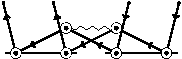
\includegraphics[height=0.9cm]{ccd_d3a}
  };
\end{tikzpicture}
+
\begin{tikzpicture}[baseline=-2.5pt,every node/.style={inner sep=0pt,outer sep=0pt}]
  \node at (0,0) {
    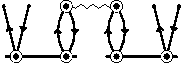
\includegraphics[height=0.9cm]{ccd_d3b}
  };
\end{tikzpicture}
+
\begin{tikzpicture}[baseline=-2.5pt,every node/.style={inner sep=0pt,outer sep=0pt}]
  \node at (0,0) {
    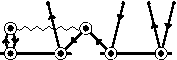
\includegraphics[height=0.9cm]{ccd_d3d}
  };
\end{tikzpicture}
+
\begin{tikzpicture}[baseline=-2.5pt,every node/.style={inner sep=0pt,outer sep=0pt}]
  \node at (0,0) {
    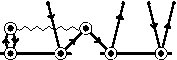
\includegraphics[height=0.9cm]{ccd_d3c}
  };
\end{tikzpicture}
+
\begin{tikzpicture}[baseline=-2.5pt,every node/.style={inner sep=0pt,outer sep=0pt}]
  \node at (0,0) {
    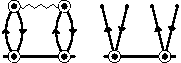
\includegraphics[height=0.9cm]{ccd_d3e}
  };
\end{tikzpicture}
\\
\updownarrow\hspace{1pt}&
\\
  \tfr{1}{2}
  \ip{\F_{ij}^{ab}|H_{\text{c}}\,T_2^2|\F}
=&\
  (\tfr{1}{2})^2\,
  \ol{g}_{kl}^{cd}
  t_{ab}^{kl}
  t_{cd}^{ij}
+
  \tfr{1}{2}
  \op{P}_{(a/b)}^{(i/j)}
  \ol{g}_{kl}^{cd}
  t_{ac}^{ik}
  t_{db}^{lj}
-
  \tfr{1}{2}
  \op{P}_{(a/b)}\,
  \ol{g}_{kl}^{cd}
  t_{ca}^{kl}
  t_{db}^{ij}
-
  \tfr{1}{2}
  \op{P}^{(i/j)}
  \ol{g}_{kl}^{cd}
  t_{cd}^{ki}
  t_{ab}^{lj}
+
  E_{\text{c}}\,
  t_{ab}^{ij}
\end{align*}
In the last term, we have substituted in the CCD energy expression, which is the same graph as the CID energy expression.
\begin{align}
\label{eq:ccd-energy-expression}
  E_{\text{c}}
=
\diagram[top, bottom]{
%middle
  \node at (0,0.3) {
  $\left(
  \diagram{
    \draw (-0.5,0) node[circlex](f){} -- (0,0) node[ddot=white](f1){};
    \draw[->-] (f1) to ++(0,+0.5);
    \draw[-<-] (f1) to ++(0,-0.5);
  }
  +
  \diagram{
    \interaction{2}{g}{(0,0)}{ddot=white}{sawtooth};
    \draw[->-] (g1) to ++(0,+0.5);
    \draw[-<-] (g1) to ++(0,-0.5);
    \draw[->-] (g2) to ++(0,+0.5);
    \draw[-<-] (g2) to ++(0,-0.5);
  }\right)$
  };
%bottom
  \interaction{2}{c}{(-0.5,-0.75)}{ddot}{overhang};
  \draw[->-] (c1) to ++(-0.25,+0.5);
  \draw[-<-] (c1) to ++(+0.25,+0.5);
  \draw[->-] (c2) to ++(-0.25,+0.5);
  \draw[-<-] (c2) to ++(+0.25,+0.5);
}
=
\diagram{
  \interaction{2}{g}{(0,+0.5)}{ddot}{sawtooth};
  \interaction{2}{c}{(0,-0.5)}{ddot}{overhang};
  \draw[-<-,bend right] (g1) to (c1);
  \draw[->-,bend left ] (g1) to (c1);
  \draw[-<-,bend right] (g2) to (c2);
  \draw[->-,bend left ] (g2) to (c2);
}
=
  (\tfr{1}{2})^2
  \ol{g}_{ij}^{ab}
  t_{ab}^{ij}
\end{align}
Note that the term $E_{\text{c}} t_{ab}^{ij}$ actually cancels with the right-hand side of the projected Schr\"odinger equation.
Since this is the only unlinked graph in the expansion, we can write the amplitude equation as
\begin{align}
  \ip{\F_{ij}^{ab}|H_{\text{c}}\text{exp}(T_2)|\F}_{\text{L}}
=
  0
\end{align}
where the subscript indicates that only linked graphs are included.
This cancellation of unlinked terms is a general feature of coupled-cluster theory.
Finally, note that when Brillouin's theorem holds the second and third terms in eq~\ref{eq:cid-coefficient-equations} become
\begin{align*}
  \op{P}_{(a/b)}
  f_a^c
  t_{cb}^{ij}
-
  \op{P}^{(i/j)}
  f_k^i
  t_{ab}^{kj}
=
-
  (\ev_i + \ev_j - \ev_a - \ev_b)
  t_{ab}^{ij}
\end{align*}
where $\{\ev_p=f_p^p\}$ are canonical Hartree-Fock orbital energies.
Subtracting this contribution from both sides leads to
\begin{align}
\label{eq:ccd-amplitude-equation-final}
  t_{ab}^{ij}
=
  (\mc{E}_{ab}^{ij})^{-1}
  \ip{\F_{ij}^{ab}|(H_{\text{c}} - f_p^p\tl{a}^p_p)\text{exp}(T_2)|\F}_{\text{L}}
&&
  \mc{E}_{ab}^{ij}
\equiv
  \ev_i + \ev_j - \ev_a - \ev_b
\end{align}
which is the standard form for the $T_2$ amplitude equation.
\end{ex}

%% Define resolvent line
% \begin{dfn}
% \thmtitle{Resolvent line}
% Complete contractions through a  \textit{resolvent line}
% $
% \resolventline[0.6]{}\hspace{3pt}
% $
% are defined as follows.
% \begin{align*}
% &&
%   \gno{
%   \ctr[4]
%     {}
%     {a}
%     {^{i_1}\cd a^{i_k}a_{a_1}\cd a_{a_k}\,a^{b_1}\cd a^{b_k}a_{j_1}\cd }
%     {a}
%   \ctr[3]
%     {a^{i_1}\cd}
%     {a}
%     {^{i_k}a_{a_1}\cd a_{a_k}\,a^{b_1}\cd a^{b_k}}
%     {a}
%   \ctr[2]
%     {a^{i_1}\cd a^{i_k}}
%     {a}
%     {_{a_1}\cd a_{a_k}\,a^{b_1}\cd}
%     {a}
%   \ctr[1]
%     {a^{i_1}\cd a^{i_k}a_{a_1}\cd}
%     {a}
%     {_{a_k}\,}
%     {a}
%   a^{i_1}\cd a^{i_k}
%   a_{a_1}\cd a_{a_k}
%   \resolventline[1.3]{}\,
%   a^{b_1}\cd a^{b_k}
%   a_{j_1}\cd a_{j_k}
%   }
% \equiv
%   \fr{\gno{
%     \ctr[4]
%       {}
%       {a}
%       {^{i_1}\cd a^{i_k}a_{a_1}\cd a_{a_k}a^{b_1}\cd a^{b_k}a_{j_1}\cd }
%       {a}
%     \ctr[3]
%       {a^{i_1}\cd}
%       {a}
%       {^{i_k}a_{a_1}\cd a_{a_k}a^{b_1}\cd a^{b_k}}
%       {a}
%     \ctr[2]
%       {a^{i_1}\cd a^{i_k}}
%       {a}
%       {_{a_1}\cd a_{a_k}a^{b_1}\cd}
%       {a}
%     \ctr[1]
%       {a^{i_1}\cd a^{i_k}a_{a_1}\cd}
%       {a}
%       {_{a_k}}
%       {a}
%     a^{i_1}\cd a^{i_k}
%     a_{a_1}\cd a_{a_k}
%     a^{b_1}\cd a^{b_k}
%     a_{j_1}\cd a_{j_k}
%   }}{
%     \mc{E}_{a_1\cd a_k}^{i_1\cd i_k}
%   }
% &\hspace{0.5cm}&
%   \mc{E}_{a_1\cd a_k}^{i_1\cd i_k}
% \equiv
%   \sum_{r=1}^k
%   \ev_{i_r}
% -
%   \sum_{r=1}^k
%   \ev_{a_r}
% \end{align*}
% This can be denoted in a graph by drawing a horizontal dotted line through several contraction lines.
% \end{dfn}

\begin{ex}
Using the notion of a resolvent line, equation \ref{eq:ccd-amplitude-equation-final} can be written in diagram notation as follows.
\begin{align}
\nonumber
\diagram{
  \interaction{2}{t}{(0,-0.5)}{ddot}{overhang};
  \draw[->-] (t1) to ++(-0.25,1) node[smalldot] {};
  \draw[-<-] (t1) to ++(+0.25,1) node[smalldot] {};
  \draw[->-] (t2) to ++(-0.25,1) node[smalldot] {};
  \draw[-<-] (t2) to ++(+0.25,1) node[smalldot] {};
}
=&\
\diagram{
  \interaction{2}{g}{(0,-0.5)}{ddot}{sawtooth};
  \draw[->-] (g1) to ++(-0.25,1) node[smalldot] {};
  \draw[-<-] (g1) to ++(+0.25,1) node[smalldot] {};
  \draw[->-] (g2) to ++(-0.25,1) node[smalldot] {};
  \draw[-<-] (g2) to ++(+0.25,1) node[smalldot] {};
  \draw[thick,flexdotted] (-0.4,+0.35) to ++(1.8,0);
}
+
\diagram{
  \interaction{2}{t}{(0,-0.5)}{ddot}{overhang};
  \draw[->-=0.25,->-=0.75] (t1) to node[midway,ddot] (g1) {}
    ++(-0.25,1) node[smalldot] {};
  \draw[-<-=0.7] (t1) to ++(+0.25,1) node[smalldot] {};
  \draw[->-=0.25,->-=0.75] (t2) to node[midway,ddot] (g2) {}
    ++(-0.25,1) node[smalldot] {};
  \draw[-<-=0.7] (t2) to ++(+0.25,1) node[smalldot] {};
  \draw[sawtooth] (g1)--(g2);
  \draw[thick,flexdotted] (-0.4,+0.35) to ++(1.8,0);
}
+
\diagram{
  \interaction{2}{t}{(0,-0.5)}{ddot}{overhang};
  \draw[-<-=0.25,-<-=0.75] (t1) to node[midway,ddot] (g1) {}
    ++(-0.25,1) node[smalldot] {};
  \draw[->-=0.7] (t1) to ++(+0.25,1) node[smalldot] {};
  \draw[-<-=0.25,-<-=0.75] (t2) to node[midway,ddot] (g2) {}
    ++(-0.25,1) node[smalldot] {};
  \draw[->-=0.7] (t2) to ++(+0.25,1) node[smalldot] {};
  \draw[sawtooth] (g1)--(g2);
  \draw[thick,flexdotted] (-0.4,+0.35) to ++(1.8,0);
}
+
\diagram{
  \interaction{2}{t}{(0,-0.5)}{ddot}{overhang};
  \interaction{2}{g}{(1,+0.0)}{ddot}{sawtooth};
  \draw[->-] (t1) to ++(-0.25,1) node[smalldot] {};
  \draw[-<-] (t1) to ++(+0.25,1) node[smalldot] {};
  \draw[->-,bend left] (t2) to (g1);
  \draw[-<-,bend right] (t2) to (g1);
  \draw[->-] (g2) to ++(-0.25,0.5) node[smalldot] {};
  \draw[-<-] (g2) to ++(+0.25,0.5) node[smalldot] {};
  \draw[thick,flexdotted] (-0.4,+0.35) to ++(2.8,0);
}
+
\diagram{
  \interaction{2}{ta}{(0,-0.5)}{ddot}{overhang};
  \interaction{2}{tb}{(2,-0.5)}{ddot}{overhang};
  \interaction{2}{g}{(1,0)}{ddot}{sawtooth};
  \draw[->-=0.7] (ta1) to ++(-0.25,1) node[smalldot] {};
  \draw[-<-=0.3] (ta1) to (g1);
  \draw[->-=0.7] (ta2) to ++(-0.25,1) node[smalldot] {};
  \draw[-<-=0.3] (ta2) to (g2);
  \draw[->-=0.3] (tb1) to (g1);
  \draw[-<-=0.7] (tb1) to ++(+0.25,1) node[smalldot] {};
  \draw[->-=0.3] (tb2) to (g2);
  \draw[-<-=0.7] (tb2) to ++(+0.25,1) node[smalldot] {};
  \draw[thick,flexdotted] (-0.4,+0.35) to ++(3.8,0);
}
\\&\
\label{eq:ccd-amplitude-equations-final-diagrammatic}
+
\diagram{
  \interaction{2}{ta}{(0,-0.5)}{ddot}{overhang};
  \interaction{2}{tb}{(2,-0.5)}{ddot}{overhang};
  \interaction{2}{g}{(1,0)}{ddot}{sawtooth};
  \draw[->-] (ta1) to ++(-0.25,1) node[smalldot] {};
  \draw[-<-] (ta1) to ++(+0.25,1) node[smalldot] {};
  \draw[->-,bend left]  (ta2) to (g1);
  \draw[-<-,bend right] (ta2) to (g1);
  \draw[->-,bend left]  (tb1) to (g2);
  \draw[-<-,bend right] (tb1) to (g2);
  \draw[->-] (tb2) to ++(-0.25,1) node[smalldot] {};
  \draw[-<-] (tb2) to ++(+0.25,1) node[smalldot] {};
  \draw[thick,flexdotted] (-0.4,+0.35) to ++(3.8,0);
}
+
\diagram{
  \interaction{2}{ta}{(0,-0.5)}{ddot}{overhang};
  \interaction{2}{tb}{(2,-0.5)}{ddot}{overhang};
  \draw[sawtooth] (0,0) node[ddot] (g1) {} to (1.5,0) node[ddot] (g2) {};
  \draw[->-,bend left]  (ta1) to (g1);
  \draw[-<-,bend right] (ta1) to (g1);
  \draw[->-=0.7] (ta2) to ++(-0.25,1) node[smalldot] {};
  \draw[-<-] (ta2) to (g2);
  \draw[->-] (tb1) to (g2);
  \draw[-<-=0.7] (tb1) to ++(+0.25,1) node[smalldot] {};
  \draw[->-] (tb2) to ++(-0.25,1) node[smalldot] {};
  \draw[-<-] (tb2) to ++(+0.25,1) node[smalldot] {};
  \draw[thick,flexdotted] (0.6,+0.35) to ++(2.8,0);
}
+
\diagram{
  \interaction{2}{ta}{(0,-0.5)}{ddot}{overhang};
  \interaction{2}{tb}{(2,-0.5)}{ddot}{overhang};
  \draw[sawtooth] (0,0) node[ddot] (g1) {} to (1.5,0) node[ddot] (g2) {};
  \draw[->-,bend left]  (ta1) to (g1);
  \draw[-<-,bend right] (ta1) to (g1);
  \draw[-<-=0.7] (ta2) to ++(-0.25,1) node[smalldot] {};
  \draw[->-] (ta2) to (g2);
  \draw[-<-] (tb1) to (g2);
  \draw[->-=0.7] (tb1) to ++(+0.25,1) node[smalldot] {};
  \draw[-<-] (tb2) to ++(-0.25,1) node[smalldot] {};
  \draw[->-] (tb2) to ++(+0.25,1) node[smalldot] {};
  \draw[thick,flexdotted] (0.6,+0.35) to ++(2.8,0);
}
\end{align}
This equation is typically solved in an iterative procedure that updates the amplitudes by substituting the previous iteration's amplitudes into the right-hand side, starting with ${}^{[0]}t_{ab}^{ij}=0$ as an initial guess.
\end{ex}

\begin{rmk}
\thmtitle{The CEPA$_0$ and MP2 amplitude equations}
If the $T_2$ amplitudes are small, the CCD exponential, $\text{exp}(T_2)=1 + T_2 + \tfr{1}{2}T_2^2 + \ld$, can be approximated by the linear terms or even just the constant term, leading to the \textit{coupled~electron-pair~approximation~zero (CEPA$_0$)} and \textit{second-order M\o ller-Plesset perturbation theory (MP2)} methods.
Assuming Brillouin's theorem and writing $V$ for the electron repulsion operator,
$
  \tfr{1}{4}
  \ol{g}_{pq}^{rs}
  \tl{a}^{pq}_{rs}
$,
these amplitude equations are
\begin{align}
\label{eq:mp2-amplitude-equations}
  \text{MP2}:\hspace{5pt}
  t_{ab}^{ij}
=&\
  (\mc{E}_{ab}^{ij})^{-1}
  \ip{\F_{ij}^{ab}|V|\F}_{\text{L}}
=
\diagram{
  \interaction{2}{g}{(0,-0.5)}{ddot}{sawtooth};
  \draw[->-] (g1) to ++(-0.25,1) node[smalldot] {};
  \draw[-<-] (g1) to ++(+0.25,1) node[smalldot] {};
  \draw[->-] (g2) to ++(-0.25,1) node[smalldot] {};
  \draw[-<-] (g2) to ++(+0.25,1) node[smalldot] {};
  \draw[thick,flexdotted] (-0.4,+0.35) to ++(1.8,0);
}
\\
\label{eq:cepa-amplitude-equations}
  \text{CEPA$_0$}:\hspace{5pt}
  t_{ab}^{ij}
=&\
  (\mc{E}_{ab}^{ij})^{-1}
  \ip{\F_{ij}^{ab}|V(1 + T_2)|\F}_{\text{L}}
=
\diagram{
  \interaction{2}{g}{(0,-0.5)}{ddot}{sawtooth};
  \draw[->-] (g1) to ++(-0.25,1) node[smalldot] {};
  \draw[-<-] (g1) to ++(+0.25,1) node[smalldot] {};
  \draw[->-] (g2) to ++(-0.25,1) node[smalldot] {};
  \draw[-<-] (g2) to ++(+0.25,1) node[smalldot] {};
  \draw[thick,flexdotted] (-0.4,+0.35) to ++(1.8,0);
}
+
\diagram{
  \interaction{2}{t}{(0,-0.5)}{ddot}{overhang};
  \draw[->-=0.25,->-=0.75] (t1) to node[midway,ddot] (g1) {}
    ++(-0.25,1) node[smalldot] {};
  \draw[-<-=0.7] (t1) to ++(+0.25,1) node[smalldot] {};
  \draw[->-=0.25,->-=0.75] (t2) to node[midway,ddot] (g2) {}
    ++(-0.25,1) node[smalldot] {};
  \draw[-<-=0.7] (t2) to ++(+0.25,1) node[smalldot] {};
  \draw[sawtooth] (g1)--(g2);
  \draw[thick,flexdotted] (-0.4,+0.35) to ++(1.8,0);
}
+
\diagram{
  \interaction{2}{t}{(0,-0.5)}{ddot}{overhang};
  \draw[-<-=0.25,-<-=0.75] (t1) to node[midway,ddot] (g1) {}
    ++(-0.25,1) node[smalldot] {};
  \draw[->-=0.7] (t1) to ++(+0.25,1) node[smalldot] {};
  \draw[-<-=0.25,-<-=0.75] (t2) to node[midway,ddot] (g2) {}
    ++(-0.25,1) node[smalldot] {};
  \draw[->-=0.7] (t2) to ++(+0.25,1) node[smalldot] {};
  \draw[sawtooth] (g1)--(g2);
  \draw[thick,flexdotted] (-0.4,+0.35) to ++(1.8,0);
}
+
\diagram{
  \interaction{2}{t}{(0,-0.5)}{ddot}{overhang};
  \interaction{2}{g}{(1,+0.0)}{ddot}{sawtooth};
  \draw[->-] (t1) to ++(-0.25,1) node[smalldot] {};
  \draw[-<-] (t1) to ++(+0.25,1) node[smalldot] {};
  \draw[->-,bend left] (t2) to (g1);
  \draw[-<-,bend right] (t2) to (g1);
  \draw[->-] (g2) to ++(-0.25,0.5) node[smalldot] {};
  \draw[-<-] (g2) to ++(+0.25,0.5) node[smalldot] {};
  \draw[thick,flexdotted] (-0.4,+0.35) to ++(2.8,0);
}
\end{align}
where the MP2 amplitude is usually denoted ${}^{(1)}t_{ab}^{ij}$ because it is correct to first order in perturbation theory.
Note that eq~\ref{eq:mp2-amplitude-equations} specifies the MP2 amplitudes directly,
$
  {}^{(1)}t_{ab}^{ij}
=
  (\mc{E}_{ab}^{ij})^{-1}\,\ol{g}_{ab}^{ij}
$,
and requires no iterative solution.
Substituting these amplitudes into equation \ref{eq:ccd-energy-expression} gives the MP2 energy, which has contributions up to second order in perturbation theory.
\begin{align}
  E_{\text{c}}\ord{2}
=
\diagram{
  \interaction{2}{g}{(0,+0.5)}{ddot}{sawtooth};
  \interaction{2}{c}{(0,-0.5)}{ddot}{overhang};
  \draw[-<-,bend right] (g1) to (c1);
  \draw[->-,bend left ] (g1) to (c1);
  \draw[-<-,bend right] (g2) to (c2);
  \draw[->-,bend left ] (g2) to (c2);
  \node[right = 3pt of c2] (order) {$(1)$};
}
=
\diagram{
  \interaction{2}{g}{(0,+0.5)}{ddot}{sawtooth};
  \interaction{2}{c}{(0,-0.5)}{ddot}{sawtooth};
  \draw[-<-=0.4,bend right] (g1) to (c1);
  \draw[->-=0.6,bend left ] (g1) to (c1);
  \draw[-<-=0.4,bend right] (g2) to (c2);
  \draw[->-=0.6,bend left ] (g2) to (c2);
  \draw[thick,flexdotted] (-0.4,0) to ++(1.8,0);
}
=
  \fr{1}{4}
  \sum_{ijab}
  \fr{\ol{g}_{ab}^{ij}\ol{g}_{ij}^{ab}}{\mc{E}_{ab}^{ij}}
\end{align}
\end{rmk}

\chapter{Traditional coupled-cluster theory}

\begin{dfn}\label{dfn:cc-effective-hamiltonian}
\thmtitle{Traditional coupled-cluster theory}
A \textit{wave operator} maps a determinant into a correlated wavefunction, $\Y=\W\F$.
The \textit{coupled-cluster Ansatz} is characterized by an exponential parametrization of the wave operator.
\begin{align}
\label{eq:cc-effective-hamiltonian}
  H_{\text{c}}\Y_{\text{CC}}
=
  E_{\text{c}}\Y_{\text{CC}}
&&
  \Y_{\text{CC}}
\equiv
  \text{exp}(T)
  \F
&&
  T
\equiv
  T_1
+
  T_2
+
  \cd
+
  T_n
&&
  T_k
\equiv
  (\tfr{1}{k!})^2
  t_{a_1\cd a_k}^{i_1\cd i_k}
  \tl{a}^{a_1\cd a_k}_{i_1\cd i_k}
\end{align}
The coupled-cluster Schr\"odinger equation can be projected onto the determinant basis to arrive at a series of equations
\begin{align}
\label{eq:projected-cc-equations}
  \ip{\F|H_{\text{c}}|\Y_{\text{CC}}}
=
  E_{\text{c}}
&&
  \ip{\F_{ij\cd}^{ab\cd}|H_{\text{c}}|\Y_{\text{CC}}}
=
  E_{\text{c}}
  \ip{\F_{ij\cd}^{ab\cd}|\Y_{\text{CC}}}
\end{align}
which specify the coupled-cluster energy and the \textit{amplitudes}, $t_{ab\cd}^{ij\cd}$.
A different approach, known as \textit{traditional coupled-cluster (TCC) theory}, first multiplies the Schr\"odinger equation on the left by the inverse of the wave operator
\begin{align}
  \ol{H}_{\text{c}}
  \F
=
  E_{\text{c}}
  \F
&&
  \ol{H}_{\text{c}}
\equiv
  \text{exp}(-T)
  H_{\text{c}}\,
  \text{exp}(T)
\end{align}
to define an \textit{effective Hamiltonian}, $\ol{H}_{\text{c}}$.
The eigenvalue of this similarity-transformed\footnote{See \url{https://en.wikipedia.org/wiki/Matrix_similarity}.} Hamiltonian is the exact correlation energy, $E_{\text{c}}$, but its eigenstate is the reference determinant, $\F$, rather than the correlated wavefunction.
Note that, unlike the true Hamiltonian, $\ol{H}_{\text{c}}$ is non-Hermitian.
Projection onto the determinant basis yields energy and amplitude equations
\begin{align}
\label{eq:traditional-cc-equations}
  \ip{\F|\ol{H}_{\text{c}}|\F}
=
  E_{\text{c}}
&&
  \ip{\F_{ij\cd}^{ab\cd}|\ol{H}_{\text{c}}|\F}
=
  0
\end{align}
which look similar to eq~\ref{eq:projected-cc-equations}, except that the right-hand side of the amplitude equations is now zero.
The next few results show that the TCC similarity transformation removes disconnected terms in eq~\ref{eq:projected-cc-equations}, of which $E_{\text{c}}t_{ab\cd}^{ij\cd}$ is an example.
\end{dfn}

\begin{thm}\label{thm:hausdorff}
\thmtitle{The Hausdorff Expansion}
\thmstatement{
$\ds{
  e^{- X}Ye^{X}
=
  \sum_{n=0}^\infty
  \fr{1}{n!}
  [\,\cdot\,, X]^n(Y)
}$
}\,\footnote{
$
  [\,\cdot\,, X]^n(Y)
$
denotes a nested commutator,
$
  [\cd[[Y,X],X]\cd,X]
$.
For $n=0$, we define
$
  [\,\cdot\,, X]^0(Y)
\equiv
  Y
$.
}\vspace{5pt}
\thmproof{
  This follows from
  $
    \pd{^n}{\la^n}
    e^{-\la X}Ye^{\la X}
  =
    [\,\cdot\,, X]^n(
    e^{-\la X}Ye^{\la X}
    )
  $,
  which we will prove by induction.
  This is trivially true for $n=0$.
  Assuming it holds for $n$, the following shows that it also holds for $n+1$, completing the induction.
\begin{align*}
  \tpd{^{n+1}}{\la^{n+1}}
  e^{-\la X}Ye^{\la X}
=
  [\,\cdot\,, X]^n(
  \tpd{}{\la}
  e^{-\la X}Ye^{\la X}
  )
=
  [\,\cdot\,, X]^n(
    e^{-\la X}Ye^{\la X} X
  -
    X e^{-\la X}Ye^{\la X}
  )
=
  [\,\cdot\,, X]^{n+1}(
    e^{-\la X}Ye^{\la X}
  )
\end{align*}
  Substituting this result into a Taylor expansion of
  $
    e^{-\la X}Ye^{\la X}
  $
  about
  $\la=0$
  evaluated at
  $\la=1$
  completes the proof.
}
\end{thm}

\begin{ex}
The Hausdorff expansion can be used to express the TCC effective Hamiltonian in powers of $T$.
\begin{align*}
  \ol{H}_{\text{c}}
=
  \text{exp}(-T)
  H_{\text{c}}\,
  \text{exp}(T)
=
  H_{\text{c}}
+
  [H_{\text{c}}, T]
+
  \tfr{1}{2!}
  [[H_{\text{c}}, T], T]
+
  \tfr{1}{3!}
  [[[H_{\text{c}}, T], T], T]
+
  \tfr{1}{4!}
  [[[[H_{\text{c}}, T], T], T], T]
+
  \cd
\end{align*}
This expansion can be further simplified by analyzing the commutators with $T$ using Wick's theorem.
\end{ex}

\begin{prop}\label{prop:wicks-theorem-for-commutators}
\thmstatement{
If $Q$ and $Q'$ are normal ordered and one of them has an even operator count,
$
  [Q,Q']
=
  \gno{
    \ctr{}{Q}{}{Q}
    QQ'
  }
-
  \gno{
    \ctr{}{Q}{'}{Q}
    Q'Q
  }
$.%
}\vspace{2pt}%
\thmproof{
By Wick's theorem,
$
  QQ'
-
  Q'Q
=
  \gno{QQ'}
+
  \gno{
    \ctr{}{Q}{}{Q}
    QQ'
  }
-
  \gno{Q'Q}
-
  \gno{
    \ctr{}{Q}{'}{Q}
    Q'Q
  }
$.
The proposition follows from the fact that
$
  \gno{QQ'}
=
  \gno{Q'Q}
$
when one of the strings contains an even number of operators.
}
\end{prop}

\begin{cor}
\label{cor:tcc-similarity-transformation-connected}
\thmstatement{
  TCC similarity-transformed operators,
  $
    \ol{W}
  \equiv
    \text{exp}(-T)
    W
    \text{exp}(T)
  $,
  can be evaluated as
  $
    \ol{W}
  =
    (
      W\,
      \text{exp}(T)
    )_{\text{C}}
  $,
  where the subscript $\text{C}$ denotes a restriction to connected diagrams.
}
\thmproof{
  \Cref{prop:wicks-theorem-for-commutators} implies
$
  [W,T]
=
\gno{
  \ctr{}{W}{}{T}
  WT
}
$
and, by straightforward induction,
$
  [\,\cdot\,,T]^n(W)
=
\gno{
  \ctr[1.4]{}{W}{TT\cd}{T}
  \ctr[0.7]{}{W}{T}{T}
  \ctr[0.0]{}{W}{}{T}
  WTT\cd T
}
=
  (WT^n)_{\text{C}}
$,
since
$T$
has no contractions with operators to its right.\footnote{This is easily seen from the diagram.  It comes from the fact that $T$ is composed entirely of quasi-particle creation operators.}
  Applying \cref{thm:hausdorff} to $\ol{W}$ and using this result completes the proof.
}
\end{cor}


\begin{rmk}\label{rmk:connected-expansion}
Applying \cref{cor:tcc-similarity-transformation-connected} to the coupled-cluster effective Hamiltonian gives the following expansion
\begin{align}
  \ol{H}_{\text{c}}
=
  (H_{\text{c}}\,
   \text{exp}(T))_{\text{C}}
=
  (
    H_{\text{c}}
  +
    H_{\text{c}}
    T
  +
    \tfr{1}{2!}
    H_{\text{c}}
    T^2
  +
    \tfr{1}{3!}
    H_{\text{c}}
    T^3
  +
    \tfr{1}{4!}
    H_{\text{c}}
    T^4
  )_{\text{C}}
\end{align}
which ends at the fourth power because $H_{\text{c}}$ is a linear combination of one- and two-particle operators, which can contract at most two and four $T$'s, respectively.
Using this result, the energy and amplitude equations are often written as
\begin{align}
\label{eq:traditional-cc-equations-2}
  \ip{\F|H_{\text{c}}\,\text{exp}(T)|\F}_{\text{C}}
=
  E_{\text{c}}
&&
  \ip{\F_{ij\cd}^{ab\cd}|H_{\text{c}}\,\text{exp}(T)|\F}_{\text{C}}
=
  0
\end{align}
where the subscript $\text{C}$ on the expectation value ket is shorthand for
$
  \ip{\F_{ij\cd}^{ab\cd}|(H_{\text{c}}\,\text{exp}(T))_{\text{C}}|\F}
$.
\end{rmk}


\begin{ntt}
The following is suggested notation for the diagonal and off-diagonal contributions to the Fock operator.
\begin{align}
\diagram{
  \draw (-0.5,0) node[circlex] (h) {} -- (0,0) node[ddot=white] (h1) {};
  \draw[->-] (h1) to ++(0,+0.5);
  \draw[-<-] (h1) to ++(0,-0.5);
}
=
\diagram{
  \draw (-0.5,0) node[circlez] (h) {} -- (0,0) node[ddot=white] (h1) {};
  \draw[->-] (h1) to ++(0,+0.5);
  \draw[-<-] (h1) to ++(0,-0.5);
}
+
\diagram{
  \draw (-0.5,0) node[circlep] (h) {} -- (0,0) node[ddot=white] (h1) {};
  \draw[->-] (h1) to ++(0,+0.5);
  \draw[-<-] (h1) to ++(0,-0.5);
}
&&
\diagram{
  \draw (-0.5,0) node[circlez] (h) {} -- (0,0) node[ddot=white] (h1) {};
  \draw[->-] (h1) to ++(0,+0.5);
  \draw[-<-] (h1) to ++(0,-0.5);
}
\equiv
  H_0
&&
\diagram{
  \draw (-0.5,0) node[circlep] (h) {} -- (0,0) node[ddot=white] (h1) {};
  \draw[->-] (h1) to ++(0,+0.5);
  \draw[-<-] (h1) to ++(0,-0.5);
}
\equiv
  f_p^q(1-\delta_p^q)
  \tl{a}^p_q
\end{align}
so that
$
  H
=
  E_{\text{ref}}
+
\diagram{
  \draw (-0.5,0) node[circlez] (h) {} -- (0,0) node[ddot=white] (h1) {};
  \draw[->-] (h1) to ++(0,+0.35);
  \draw[-<-] (h1) to ++(0,-0.35);
}
+
\diagram{
  \draw (-0.5,0) node[circlep] (h) {} -- (0,0) node[ddot=white] (h1) {};
  \draw[->-] (h1) to ++(0,+0.35);
  \draw[-<-] (h1) to ++(0,-0.35);
}
+
\diagram{
  \interaction{2}{g}{(0,0)}{ddot=white}{sawtooth};
  \draw[->-] (g1) to ++(0,+0.35);
  \draw[-<-] (g1) to ++(0,-0.35);
  \draw[->-] (g2) to ++(0,+0.35);
  \draw[-<-] (g2) to ++(0,-0.35);
}
$\
is the full electronic Hamiltonian
and
$
  V_{\text{c}}
=
\diagram{
  \draw (-0.5,0) node[circlep] (h) {} -- (0,0) node[ddot=white] (h1) {};
  \draw[->-] (h1) to ++(0,+0.35);
  \draw[-<-] (h1) to ++(0,-0.35);
}
+
\diagram{
  \interaction{2}{g}{(0,0)}{ddot=white}{sawtooth};
  \draw[->-] (g1) to ++(0,+0.35);
  \draw[-<-] (g1) to ++(0,-0.35);
  \draw[->-] (g2) to ++(0,+0.35);
  \draw[-<-] (g2) to ++(0,-0.35);
}
$.
Note that
\begin{align*}
\diagram{
  \draw (-0.5,0) node[circlez] (h) {} -- (0,0) node[ddot=white] (h1) {};
  \draw[->-] (h1) to ++(0,+0.5);
  \draw[-<-] (h1) to ++(0,-0.5);
}
=
\diagram{
  \draw (-0.5,0) node[circlez] (h) {} -- (0,0) node[ddot] (h1) {};
  \draw[->-] (h1) to ++(0,+0.5);
  \draw[-<-] (h1) to ++(0,-0.5);
}
+
\diagram{
  \draw (-0.5,0) node[circlez] (h) {} -- (0,0) node[ddot] (h1) {};
  \draw[-<-] (h1) to ++(0,+0.5);
  \draw[->-] (h1) to ++(0,-0.5);
}
&&
\diagram{
  \draw (-0.5,0) node[circlep] (h) {} -- (0,0) node[ddot=white] (h1) {};
  \draw[->-] (h1) to ++(0,+0.5);
  \draw[-<-] (h1) to ++(0,-0.5);
}
=
\diagram{
  \draw (-0.5,0) node[circlep] (h) {} -- (0,0) node[ddot] (h1) {};
  \draw[->-] (h1) to ++(0,+0.5);
  \draw[-<-] (h1) to ++(0,-0.5);
}
+
\diagram{
  \draw (-0.5,0) node[circlep] (h) {} -- (0,0) node[ddot] (h1) {};
  \draw[->-] (h1) to ++(-0.25,+0.5);
  \draw[-<-] (h1) to ++(+0.25,+0.5);
}
+
\diagram{
  \draw (-0.5,0) node[circlep] (h) {} -- (0,0) node[ddot] (h1) {};
  \draw[->-] (h1) to ++(-0.25,-0.5);
  \draw[-<-] (h1) to ++(+0.25,-0.5);
}
+
\diagram{
  \draw (-0.5,0) node[circlep] (h) {} -- (0,0) node[ddot] (h1) {};
  \draw[-<-] (h1) to ++(0,+0.5);
  \draw[->-] (h1) to ++(0,-0.5);
}
\end{align*}
where the excitation level $\pm1$ contributions to $H_0$ have been omitted because its interaction tensor is diagonal.
\end{ntt}


\begin{rmk}
It can be shown that the determinant basis forms an eigenbasis for the diagonal part of the Fock operator.\footnotemark
\begin{align}
  H_0\F_{i_1\cd i_k}^{a_1\cd a_k}
=
  \mc{E}_{i_1\cd i_k}^{a_1\cd a_k}
  \F_{i_1\cd i_k}^{a_1\cd a_k}
&&
  H_0
\equiv
  f_p^p\tl{a}^p_p
&&
  \mc{E}_{q_1\cd q_k}^{p_1\cd p_k}
\equiv
  \sum_{r=1}^k
  f_{p_r}^{p_r}
-
  \sum_{r=1}^k
  f_{q_r}^{q_r}
\end{align}
Noting that $H_0$ is Hermitian, this implies
$\ip{\F_{ij\cd}^{ab\cd}|H_0\,T|\F}=\mc{E}_{ij\cd}^{ab\cd}\ip{\F_{ij\cd}^{ab\cd}|T|\F}=\mc{E}_{ij\cd}^{ab\cd}t_{ab\cd}^{ij\cd}$.
This can be used to rearrange the amplitude equation in
(\ref{eq:traditional-cc-equations-2}) as follows, which defines the working
equations used to iteratively solve TCC.%
\footnote{%
    Note that $\ip{\F_{ij\cd}^{ab\cd}|H_0\,\exp(T)|\F}_{\text{C}}=\ip{\F_{ij\cd}^{ab\cd}|H_0\,T|\F}$.
}
\begin{align}
  t_{ab\cd}^{ij\cd}
=
  (\mc{E}_{ab\cd}^{ij\cd})^{-1}
  \ip{\F_{ab\cd}^{ij\cd}|V_{\text{c}}\,\text{exp}(T)|\F}_{\text{C}}
&&
  V_{\text{c}}
\equiv
  H_{\text{c}}
-
  H_0
=
  f_p^q(1-\delta_p^q)
  \tl{a}^p_q
+
  \tfr{1}{4}
  \ol{g}_{pq}^{rs}
  \tl{a}^{pq}_{rs}
\end{align}
In M\o ller-Plesset perturbation theory, $H_0$ is known the \textit{zeroth order Hamiltonian} and $V_{\text{c}}$ is the \textit{perturbation}.
These operators are also known as the \textit{model Hamiltonian} and \textit{fluctuation potential}, respectively.
\end{rmk}
\footnotetext{
The proof is as follows.
First, note that $a^p_p\F_\si = n_p^\si \F_\si$, where $n_p^\si$ is the occupation of $\y_p$ in $\F_\si$.
By Wick's theorem, $a^p_p=\tl{a}^p_p+n_p^{\text{ref}}$, where $n_p^{\text{ref}}$ denotes the occupation of $\y_p$ in $\F$.
Therefore, $\tl{a}^p_p\F_\si = (n_p^\si - n_p^{\text{ref}})\F_\si$ and $H_0\F_\si = \pr{\sum_{p\in\F_\si}f_p^p - \sum_{p\in\F}f_p^p}\F_\si$.
}


\begin{dfn}
\thmtitle{Excitation level}
The \textit{excitation level} of a graph equals the net number of particles or quasi-particles it creates, divided by two.
For example, the quasi-particle excitation levels of the $T_1$, $T_2$ and $T_3$ operators are $1$, $2$, and $3$, respectively, and that of $\tl{a}_{abcd}^{ijkl}$ is $-4$.
A convenient rule for evaluating reference expectation values is that the total excitation level of a closed graph must balance out to zero.
\end{dfn}

\begin{ex}
The excitation levels in the quasi-particle expansions of one- and two-particle operators are as follows.
\begin{align*}
\diagram{
  \draw (-0.5,0) node[circlep] (h) {} -- (0,0) node[ddot=white] (h1) {};
  \draw[->-] (h1) to ++(0,+0.5);
  \draw[-<-] (h1) to ++(0,-0.5);
  \node at (0,-0.8) {$(0)$};
}
=&\
\diagram{
  \draw (-0.5,0) node[circlep] (h) {} -- (0,0) node[ddot] (h1) {};
  \draw[->-] (h1) to ++(0,+0.5);
  \draw[-<-] (h1) to ++(0,-0.5);
  \node at (0,-0.8) {$(0)$};
}
+
\diagram{
  \draw (-0.5,0) node[circlep] (h) {} -- (0,0) node[ddot] (h1) {};
  \draw[->-] (h1) to ++(-0.25,+0.5);
  \draw[-<-] (h1) to ++(+0.25,+0.5);
  \node at (0,-0.8) {$(+1)$};
}
+
\diagram{
  \draw (-0.5,0) node[circlep] (h) {} -- (0,0) node[ddot] (h1) {};
  \draw[->-] (h1) to ++(-0.25,-0.5);
  \draw[-<-] (h1) to ++(+0.25,-0.5);
  \node at (0,-0.8) {$(-1)$};
}
+
\diagram{
  \draw (-0.5,0) node[circlep] (h) {} -- (0,0) node[ddot] (h1) {};
  \draw[->-] (h1) to ++(0,-0.5);
  \draw[-<-] (h1) to ++(0,+0.5);
  \node at (0,-0.8) {$(0)$};
}
\\[10pt]
\diagram{
  \interaction{2}{g}{(0,0)}{ddot=white}{sawtooth};
  \draw[->-] (g1) to ++(0,+0.5);
  \draw[-<-] (g1) to ++(0,-0.5);
  \draw[->-] (g2) to ++(0,+0.5);
  \draw[-<-] (g2) to ++(0,-0.5);
  \node at (0.5,-0.8) {$(0)$};
}
=&\
\diagram{
  \interaction{2}{g}{(0,0)}{ddot}{sawtooth};
  \draw[->-] (g1) to ++(0,+0.5);
  \draw[-<-] (g1) to ++(0,-0.5);
  \draw[->-] (g2) to ++(0,+0.5);
  \draw[-<-] (g2) to ++(0,-0.5);
  \node at (0.5,-0.8) {$(0)$};
}
+
\diagram{
  \interaction{2}{g}{(0,0)}{ddot}{sawtooth};
  \draw[->-] (g1) to ++(0,+0.5);
  \draw[-<-] (g1) to ++(0,-0.5);
  \draw[->-] (g2) to ++(-0.25,+0.5);
  \draw[-<-] (g2) to ++(+0.25,+0.5);
  \node at (0.5,-0.8) {$(+1)$};
}
+
\diagram{
  \interaction{2}{g}{(0,0)}{ddot}{sawtooth};
  \draw[->-] (g1) to ++(0,+0.5);
  \draw[-<-] (g1) to ++(0,-0.5);
  \draw[->-] (g2) to ++(-0.25,-0.5);
  \draw[-<-] (g2) to ++(+0.25,-0.5);
  \node at (0.5,-0.8) {$(-1)$};
}
+
\diagram{
  \interaction{2}{g}{(0,0)}{ddot}{sawtooth};
  \draw[->-] (g1) to ++(-0.25,+0.5);
  \draw[-<-] (g1) to ++(+0.25,+0.5);
  \draw[->-] (g2) to ++(-0.25,+0.5);
  \draw[-<-] (g2) to ++(+0.25,+0.5);
  \node at (0.5,-0.8) {$(+2)$};
}
+
\diagram{
  \interaction{2}{g}{(0,0)}{ddot}{sawtooth};
  \draw[->-] (g1) to ++(-0.25,-0.5);
  \draw[-<-] (g1) to ++(+0.25,-0.5);
  \draw[->-] (g2) to ++(-0.25,+0.5);
  \draw[-<-] (g2) to ++(+0.25,+0.5);
  \node at (0.5,-0.8) {$(0)$};
}
+
\diagram{
  \interaction{2}{g}{(0,0)}{ddot}{sawtooth};
  \draw[->-] (g1) to ++(-0.25,-0.5);
  \draw[-<-] (g1) to ++(+0.25,-0.5);
  \draw[->-] (g2) to ++(-0.25,-0.5);
  \draw[-<-] (g2) to ++(+0.25,-0.5);
  \node at (0.5,-0.8) {$(-2)$};
}
+
\diagram{
  \interaction{2}{g}{(0,0)}{ddot}{sawtooth};
  \draw[->-] (g1) to ++(0,-0.5);
  \draw[-<-] (g1) to ++(0,+0.5);
  \draw[->-] (g2) to ++(-0.25,+0.5);
  \draw[-<-] (g2) to ++(+0.25,+0.5);
  \node at (0.5,-0.8) {$(+1)$};
}
+
\diagram{
  \interaction{2}{g}{(0,0)}{ddot}{sawtooth};
  \draw[->-] (g1) to ++(0,-0.5);
  \draw[-<-] (g1) to ++(0,+0.5);
  \draw[->-] (g2) to ++(-0.25,-0.5);
  \draw[-<-] (g2) to ++(+0.25,-0.5);
  \node at (0.5,-0.8) {$(-1)$};
}
+
\diagram{
  \interaction{2}{g}{(0,0)}{ddot}{sawtooth};
  \draw[->-] (g1) to ++(0,-0.5);
  \draw[-<-] (g1) to ++(0,+0.5);
  \draw[->-] (g2) to ++(0,-0.5);
  \draw[-<-] (g2) to ++(0,+0.5);
  \node at (0.5,-0.8) {$(0)$};
}\,\,.
\end{align*}
\end{ex}


\begin{ex}
\thmtitle{The CCSDTQ equations}
Truncating the cluster operator at quadruples, $T\approx T_1 + T_2 + T_3 + T_4$, gives the CCSDTQ approximation.
The resulting singles, doubles, triples, and quadruples amplitude equations are given by\begin{align}
\nonumber
  t_a^i
=&\
  (\mc{E}_a^i)^{-1}
  \ip{\F_i^a|
    V_{\text{c}}
    (
      1
    +
      T_1
    +
      T_2
    +
      T_3
    +
      \tfr{1}{2}
      T_1^2
    +
      T_1T_2
    +
      \tfr{1}{3!}
      T_1^3
    )
  |\F}_{\text{C}}
\\[3pt]
\nonumber
  t_{ab}^{ij}
=&\
  (\mc{E}_{ab}^{ij})^{-1}
  \br{\F_{ij}^{ab}}
    V_{\text{c}}
    (
      1
    +
      T_1
    +
      T_2
    +
      T_3
    +
      T_4
    +
      \tfr{1}{2}
      T_1^2
    +
      T_1T_2
    +
      T_1T_3
    +
      \tfr{1}{2}
      T_2^2
    +
      \tfr{1}{3!}
      T_1^3
    +
      \tfr{1}{2}
      T_1^2T_2
    +
      \tfr{1}{4!}
      T_1^4
    )
  \kt{\F}_{\text{C}}
\\[3pt]
\nonumber
  t_{abc}^{ijk}
=&\
  (\mc{E}_{abc}^{ijk})^{-1}
  \br{\F_{ijk}^{abc}}
    V_{\text{c}}
    (
      T_2
    +
      T_3
    +
      T_4
    +
      T_1T_2
    +
      T_1T_3
    +
      \tfr{1}{2}
      T_2^2
    +
      T_1T_4
    +
      T_2T_3
    +
      \tfr{1}{2}
      T_1^2T_2
    +
      \tfr{1}{2}
      T_1^2T_3
    +
      \tfr{1}{2}
      T_1T_2^2
    +
      \tfr{1}{3!}
      T_1^3T_2
    )
  \kt{\F}_{\text{C}}
\\[3pt]
\nonumber
  t_{abcd}^{ijkl}
=&\
  (\mc{E}_{abcd}^{ijkl})^{-1}
  \br{\F_{ijkl}^{abcd}}
    V_{\text{c}}
    (
      T_3
    +
      T_4
    +
      T_1T_3
    +
      \tfr{1}{2}
      T_2^2
    +
      T_1T_4
    +
      T_2T_3
    +
      T_2T_4
    +
      \tfr{1}{2}
      T_3^2
    +
      \tfr{1}{2}
      T_1^2T_3
    +
      \tfr{1}{2}
      T_1T_2^2
    +
      \tfr{1}{2}
      T_1^2T_4
\\
\nonumber
&
\hphantom{
  (\mc{E}_{abcd}^{ijkl})^{-1}
  \br{\F_{ijkl}^{abcd}}
    V_{\text{c}}
    (
      T_3\
 }
    +
      T_1T_2T_3
    +
      \tfr{1}{3!}
      T_2^3
    +
      \tfr{1}{3!}
      T_1^3T_3
    +
      \tfr{1}{2!2!}
      T_1^2T_2^2
    )
  \kt{\F}_{\text{C}}
\end{align}
where several contributions to $\text{exp}(T_1+T_2+T_3+T_4)$ have been omitted either because the excitation levels do not balance or because they require one of the cluster operators to be disconnected from the Hamiltonian.
\end{ex}


\begin{dfn}
\thmtitle{Isomorphism}
For any invertible map $S:\ol{V}\rightarrow V$, we can express operators and vectors on $V$ as
\begin{align}
  A
=
  S
  \ol{A}
  S^{-1}
&&
  \kt{v}
=
  S
  \kt{\ol{v}}
&&
  \br{v}
=
  \br{\ol{v}}
  S^{-1}
\end{align}
in terms of operators and vectors on $\ol{V}$.
Note that the transformed bra and ket, $\br{\ol{v}}$ and $\kt{\ol{v}}$, corresponding to $v$ are not adjoints unless the transformation is unitary, $S^{-1}=S\dg$.
The similarity-transformed operator $\ol{A}$ retains all of the basis-independent properties of $A$, such as its trace, determinant, and eigenvalue spectrum, and its matrix elements satisfy $\ip{\ol{v}|\ol{A}|\ol{v}'}=\ip{v|A|v'}$.
More broadly, the invertibility of $S$ implies an \textit{isomorphism} between $V$ and $\ol{V}$, such that all statements about $V$ are in one-to-one correspondence with statements about $\ol{V}$ under this transformation.
\end{dfn}


\begin{rmk}
Since exponential operators are automatically invertible, the TCC wave operator defines a similarity transformation of Fock space into itself.
The image of the Schr\"odinger equation under this transformation is as follows
\begin{align}
\label{eq:similarity-transformed-schrodinger-equation}
  \ol{H}
  \kt{\ol{\Y}_k}
=
  E_k
  \kt{\ol{\Y}_k}
&&
  \br{\ol{\Y}_k}
  \ol{H}
=
  \br{\ol{\Y}_k}
  E_k
&&
\begin{array}{c@{\ }l}
  \ol{H}
&=
  \text{exp}(-T)
  H\,
  \text{exp}(T)
\\
  \kt{\ol{\Y}_k}
&=
  \text{exp}(-T)
  \kt{\Y_k}
\\
  \br{\ol{\Y}_k}
&=
  \br{\Y_k}\,
  \text{exp}(T)
\end{array}
\end{align}
where the $k\eth$ left and right eigenstates are not adjoints because $\text{exp}(T)$ is inherently non-unitary.
In TCC, $T$ is determined by the requirement that the ground-state right eigenvector of $\ol{H}$ be the reference determinant,
$
  \kt{\ol{\Y}_0}
\overset{!}{=}
  \kt{\F}
$.
\end{rmk}


\begin{dfn}
\thmtitle{Equation-of-motion coupled-cluster theory}
Expanding the left and right eigenstates of $\ol{H}$ in the determinant basis leads to the \textit{equation-of-motion (EOM) coupled-cluster equations}
\begin{align}
\begin{array}{r@{\ }lr@{\ }l}
  \ol{H}
  \,{}^kR
  \kt{\F}
&
=
  E_k
  \,{}^kR
  \kt{\F}
&
  R
&=
  R_0
+
  R_1
+
  \cd
+
  R_n
\\[7pt]
  \br{\F}
  \,{}^kL\,
  \ol{H}
&=
  \br{\F}
  \,{}^kL\,
  E_k
&
  L
&=
  L_0
+
  L_1
+
  \cd
+
  L_n
\end{array}
&&
  \ip{\F|
    {}^kL\,
    {}^lR
  |\F}
\overset{!}{=}
  \delta_{kl}
\end{align}
which are analogous to the configuration interaction eigenvalue equation, ${}^kR$ and ${}^kL$ being linear excitation and de-excitation operators analogous to $C$ and $C\dg$.
The condition on the right indicates that left and right eigenstates are chosen to form a \textit{biorthonormal system} by normalizing the overlap of the $k\eth$ left and right eigenfunctions to equal one.
Observable expectation values are given by
$
  \ip{\Y_k|W|\Y_k}
=
  \ip{\F|{}^kL\,\ol{W}\,{}^kR|\F}
$
in terms of left and right EOM coefficients.
Transition matrix elements are given by
$
  \ip{\Y_k|W|\Y_l}
=
  \ip{\F|{}^kL\,\ol{W}\,{}^lR|\F}
$.
\end{dfn}

\begin{dfn}
\thmtitle{The coupled-cluster Lagrangian}
The ground-state TCC equations are equivalent to requiring ${}^0R=1$, which implies ${}^0L_0=1$ from the biorthonormality condition.
Therefore, the ground-state left eigenvector has the form
\begin{align}
\label{eq:cc-ground-state-wave-operators}
  {}^0L
=
  1
+
  \La
&&
  \La
=
  \La_1
+
  \cd
+
  \La_n
&&
  \La_k
\equiv
  (\tfr{1}{k!})^2
  \la_{i_1\cd i_k}^{a_1\cd a_k}
  \tl{a}^{i_1\cd i_k}_{a_1\cd a_k}
\end{align}
and the ground-state energy can be written as follows, in an expression known as the \textit{coupled-cluster Lagrangian}.
\begin{align}
  \ip{\Y_0|H|\Y_0}
=
  \ip{\F|
    (
      1
    +
      \La
    )
    \ol{H}
  |\F}
\equiv
  \mc{L}(\bo{t},\bm{\la})
\end{align}
To see why this constitutes a Lagrangian, note that setting its gradient with respect to $\la_{i_1\cd i_k}^{a_1\cd a_k}$ equal to zero yields the TCC amplitude equations of eq~\ref{eq:traditional-cc-equations}.
If these are satisfied, the $\la$-dependent part of the equation vanishes and the Lagrangian returns the coupled-cluster energy:
$
  \ip{\F|\ol{H}|\F}
=
  E
$.
Therefore, the $\la$ coefficients can be viewed as Lagrange multipliers enforcing the TCC amplitude equations as a constraint.
\end{dfn}


\begin{dfn}
\thmtitle{The coupled-cluster lambda equations}
Setting the gradient of $\mc{L}$ with respect to $t_{a_1\cd a_k}^{i_1\cd i_k}$ equal to zero gives the \textit{coupled-cluster lambda equations}, which determine the Lagrange multpliers.
\begin{align}
  \br{\F}
  (
    1
  +
    \La
  )
  H_{\text{c}}\,
  \text{exp}(T)
  \kt{\F_{i_1\cd i_k}^{a_1\cd a_k}}_{\text{C}}
\overset{!}{=}
  0
\end{align}
The subscript $\text{C}$ now denotes that $H_{\text{c}}$ is connected both to the ket and to the $T$ operators.
This can be rearranged as\footnote{Note that $\ip{\F|\La H_0 T^p|\F_{i_1\cd i_k}^{a_1\cd a_k}}_{\text{C}}=0$ for $p\geq 1$, since the model Hamiltonian can only connect to one operator on either side.}
\begin{align}
  \la_{i_1\cd i_k}^{a_1\cd a_k}
=
  (\mc{E}_{a_1\cd a_k}^{i_1\cd i_k})^{-1}
  \br{\F}
  (
    1
  +
    \La
  )
  V_{\text{c}}\,
  \text{exp}(T)
  \kt{\F_{i_1\cd i_k}^{a_1\cd a_k}}_{\text{C}}
\end{align}
which sets up the iterative procedure for determining $\la_{i_1\cd i_k}^{a_1\cd a_k}$ from a given set of amplitudes.
\end{dfn}


\begin{ex}
\thmtitle{The CCSD lambda equations}
Truncating the wave operator at doubles, $T\approx T_1 + T_2$, gives the CCSD approximation.
The resulting singles and doubles lambda equations are given by the following
\begin{align*}
  \la_i^a
=&\
  (\mc{E}_a^i)^{-1}
  \br{\F}
    V_{\text{c}}\,
    (
      1
    +
      T_1
    )
  +
    \La_1
    V_{\text{c}}\,
    (
      1
    +
      T_1
    +
      T_2
    +
      \tfr{1}{2}
      T_1^2
    )
  +
    \La_2
    V_{\text{c}}\,
    (
      1
    +
      T_1
    +
      T_2
    +
      \tfr{1}{2}
      T_1^2
    +
      T_1
      T_2
    )
  \kt{\F_i^a}_{\text{C}}
\\
  \la_{ij}^{ab}
=&\
  (\mc{E}_{ab}^{ij})^{-1}
  \br{\F}
    V_{\text{c}}\,
  +
    \La_1
    V_{\text{c}}\,
    (
      1
    +
      T_1
    )
  +
    \La_2
    V_{\text{c}}\,
    (
      1
    +
      T_1
    +
      T_2
    +
      \tfr{1}{2}
      T_1^2
    )
  \kt{\F_{ij}^{ab}}_{\text{C}}
\end{align*}
where we have omitted any contributions to $\text{exp}(T_1 + T_2)$ that vanish.
\end{ex}

\begin{ex}
Assuming Brillouin's theorem holds, the CCD lambda equations are as follows.
\begin{align*}
  \la_{ij}^{ab}
  \mc{E}_{ab}^{ij}
=&\
  \ip{\F|
    V_{\text{c}}
  +
    \La_2
    V_{\text{c}}
  +
    \La_2 V_{\text{c}}T_2
  |\F_{ij}^{ab}}_{\text{C}}
\\=&\
\diagram{
  \interaction{2}{g}{(0,0.5)}{ddot}{sawtooth};
  \draw[->-] (g1) to ++(-0.25,-1) node[smalldot] {};
  \draw[-<-] (g1) to ++(+0.25,-1) node[smalldot] {};
  \draw[->-] (g2) to ++(-0.25,-1) node[smalldot] {};
  \draw[-<-] (g2) to ++(+0.25,-1) node[smalldot] {};
}
+
\diagram{
  \interaction{2}{t}{(0,0.5)}{ddot}{overhang};
  \draw[->-=0.65] (t1) to ++(-0.25,-1) node[smalldot] {};
  \draw[-<-=0.25,-<-=0.75]
      (t1)
    to
      node[ddot,midway] (g1) {}
    ++(+0.25,-1)
      node[smalldot] {};
  \draw[->-=0.65] (t2) to ++(-0.25,-1) node[smalldot] {};
  \draw[-<-=0.25,-<-=0.75]
      (t2)
    to
      node[ddot,midway] (g2) {}
    ++(+0.25,-1)
      node[smalldot] {};
   \draw[sawtooth] (g1) to (g2);
}
+
\diagram{
  \interaction{2}{t}{(0,0.5)}{ddot}{overhang};
  \draw[-<-=0.65] (t1) to ++(-0.25,-1) node[smalldot] {};
  \draw[->-=0.25,->-=0.75]
      (t1)
    to
      node[ddot,midway] (g1) {}
    ++(+0.25,-1)
      node[smalldot] {};
  \draw[-<-=0.65] (t2) to ++(-0.25,-1) node[smalldot] {};
  \draw[->-=0.25,->-=0.75]
      (t2)
    to
      node[ddot,midway] (g2) {}
    ++(+0.25,-1)
      node[smalldot] {};
   \draw[sawtooth] (g1) to (g2);
}
+
\diagram{
  \interaction{2}{t}{(0,0.5)}{ddot}{overhang};
  \interaction{2}{g}{(1,0.)}{ddot}{sawtooth};
  \draw[-<-] (t1) to ++(-0.25,-1) node[smalldot] {};
  \draw[->-] (t1) to ++(+0.25,-1) node[smalldot] {};
  \draw[->-,bend left=40 ] (g1) to (t2);
  \draw[-<-,bend right=40] (g1) to (t2);
  \draw[-<-] (g2) to ++(-0.25,-0.5) node[smalldot] {};
  \draw[->-] (g2) to ++(+0.25,-0.5) node[smalldot] {};
}
+
\diagram{
  \interaction{2}{l}{(0,0.5)}{ddot}{overhang};
  \interaction{2}{g}{(2,0.5)}{ddot}{sawtooth};
  \draw[overhang] (1.5,0) node[ddot] (t1) {} to ++(1.5,0) node[ddot] (t2) {};
  \draw[-<-=0.65] (l1) to ++(-0.25,-1) node[smalldot] {};
  \draw[->-=0.65] (l1) to ++(+0.25,-1) node[smalldot] {};
  \draw[-<-=0.65] (l2) to ++(-0.25,-1) node[smalldot] {};
  \draw[-<-] (t1) to (l2);
  \draw[->-] (t1) to (g1);
  \draw[->-=0.65] (g1) to ++(+0.25,-1) node[smalldot] {};
  \draw[-<-,bend left=40 ] (t2) to (g2);
  \draw[->-,bend right=40] (t2) to (g2);
}
+
\diagram{
  \interaction{2}{l}{(0,0.5)}{ddot}{overhang};
  \interaction{2}{g}{(2,0.5)}{ddot}{sawtooth};
  \draw[overhang] (1.5,0) node[ddot] (t1) {} to ++(1.5,0) node[ddot] (t2) {};
  \draw[->-=0.65] (l1) to ++(-0.25,-1) node[smalldot] {};
  \draw[-<-=0.65] (l1) to ++(+0.25,-1) node[smalldot] {};
  \draw[->-=0.65] (l2) to ++(-0.25,-1) node[smalldot] {};
  \draw[->-] (t1) to (l2);
  \draw[-<-] (t1) to (g1);
  \draw[-<-=0.65] (g1) to ++(+0.25,-1) node[smalldot] {};
  \draw[->-,bend left=40 ] (t2) to (g2);
  \draw[-<-,bend right=40] (t2) to (g2);
}
\\&\
+
\diagram{
  \interaction{2}{l}{(0,0.5)}{ddot}{overhang};
  \interaction{2}{g}{(2.2,0.5)}{ddot}{sawtooth};
  \interaction{2}{t}{(1.1,0.0)}{ddot}{overhang};
  \draw[->-=0.7] (l1) to ++(-0.4,-1) node[smalldot] {};
  \draw[-<-=0.3] (l1) to (t1);
  \draw[->-=0.7] (l2) to ++(-0.4,-1) node[smalldot] {};
  \draw[-<-=0.3] (l2) to (t2);
  \draw[->-=0.3] (g1) to (t1);
  \draw[-<-=0.7] (g1) to ++(+0.4,-1) node[smalldot] {};
  \draw[->-=0.3] (g2) to (t2);
  \draw[-<-=0.7] (g2) to ++(+0.4,-1) node[smalldot] {};
}
+
\diagram{
  \interaction{2}{l}{(0,0.5)}{ddot}{overhang};
  \interaction{2}{g}{(2,0.5)}{ddot}{sawtooth};
  \interaction{2}{t}{(1,0.0)}{ddot}{overhang};
  \draw[-<-=0.65] (l1) to ++(-0.25,-1) node[smalldot] {};
  \draw[->-=0.65] (l1) to ++(+0.25,-1) node[smalldot] {};
  \draw[->-,bend left=40 ] (t1) to (l2);
  \draw[-<-,bend right=40] (t1) to (l2);
  \draw[->-,bend left=40 ] (t2) to (g1);
  \draw[-<-,bend right=40] (t2) to (g1);
  \draw[-<-=0.65] (g2) to ++(-0.25,-1) node[smalldot] {};
  \draw[->-=0.65] (g2) to ++(+0.25,-1) node[smalldot] {};
}
+
\diagram{
  \interaction{2}{g}{(0,0.5)}{ddot}{sawtooth};
  \interaction{2}{l}{(2.2,0.5)}{ddot}{overhang};
  \interaction{2}{t}{(1.1,0.0)}{ddot}{overhang};
  \draw[->-=0.7] (g1) to ++(-0.4,-1) node[smalldot] {};
  \draw[-<-=0.3] (g1) to (t1);
  \draw[->-=0.7] (g2) to ++(-0.4,-1) node[smalldot] {};
  \draw[-<-=0.3] (g2) to (t2);
  \draw[->-=0.3] (l1) to (t1);
  \draw[-<-=0.7] (l1) to ++(+0.4,-1) node[smalldot] {};
  \draw[->-=0.3] (l2) to (t2);
  \draw[-<-=0.7] (l2) to ++(+0.4,-1) node[smalldot] {};
}
\\&\
+
\diagram{
  \interaction{2}{g}{(0,0.5)}{ddot}{sawtooth};
  \interaction{2}{l}{(2,0.5)}{ddot}{overhang};
  \draw[overhang] (1.5,0) node[ddot] (t1) {} to ++(1.5,0) node[ddot] (t2) {};
  \draw[-<-=0.65] (g1) to ++(-0.25,-1) node[smalldot] {};
  \draw[->-=0.65] (g1) to ++(+0.25,-1) node[smalldot] {};
  \draw[-<-=0.65] (g2) to ++(-0.25,-1) node[smalldot] {};
  \draw[-<-] (t1) to (g2);
  \draw[->-] (t1) to (l1);
  \draw[->-=0.65] (l1) to ++(+0.25,-1) node[smalldot] {};
  \draw[-<-,bend left=40 ] (t2) to (l2);
  \draw[->-,bend right=40] (t2) to (l2);
}
+
\diagram{
  \interaction{2}{g}{(0,0.5)}{ddot}{sawtooth};
  \interaction{2}{l}{(2,0.5)}{ddot}{overhang};
  \draw[overhang] (1.5,0) node[ddot] (t1) {} to ++(1.5,0) node[ddot] (t2) {};
  \draw[->-=0.65] (g1) to ++(-0.25,-1) node[smalldot] {};
  \draw[-<-=0.65] (g1) to ++(+0.25,-1) node[smalldot] {};
  \draw[->-=0.65] (g2) to ++(-0.25,-1) node[smalldot] {};
  \draw[->-] (t1) to (g2);
  \draw[-<-] (t1) to (l1);
  \draw[-<-=0.65] (l1) to ++(+0.25,-1) node[smalldot] {};
  \draw[->-,bend left=40 ] (t2) to (l2);
  \draw[-<-,bend right=40] (t2) to (l2);
}
\\=&\
  \ol{g}_{ij}^{ab}
+
  \tfr{1}{2}
  \la_{ij}^{cd}
  \ol{g}_{cd}^{ab}
+
  \tfr{1}{2}
  \la_{kl}^{ab}
  \ol{g}_{ij}^{kl}
+
  P_{(i/j)}^{(a/b)}
  \la_{ik}^{ac}
  \ol{g}_{cj}^{kb}
-
  \tfr{1}{2}
  P_{(i/j)}
  \la_{ik}^{ab}
  t_{cd}^{kl}
  \ol{g}_{jl}^{cd}
-
  \tfr{1}{2}
  P^{(a/b)}
  \la_{ij}^{ac}
  t_{cd}^{kl}
  \ol{g}_{kl}^{bd}
\\&\
+
  \tfr{1}{2^2}
  \la_{ij}^{cd}
  t_{cd}^{kl}
  \ol{g}_{kl}^{ab}
+
  P_{(i/j)}^{(a/b)}
  \la_{ik}^{ac}
  t_{cd}^{kl}
  \ol{g}_{lj}^{db}
+
  \tfr{1}{2^2}
  \ol{g}_{ij}^{cd}
  t_{cd}^{kl}
  \la_{kl}^{ab}
-
  \tfr{1}{2}
  P_{(i/j)}
  \ol{g}_{ik}^{ab}
  t_{cd}^{kl}
  \la_{jl}^{cd}
-
  \tfr{1}{2}
  P^{(a/b)}
  \ol{g}_{ij}^{ac}
  t_{cd}^{kl}
  \la_{kl}^{bd}
\end{align*}
\end{ex}

\begin{samepage}
\begin{rmk}
\thmtitle{The Hellmann-Feynman theorem}
If the Hamiltonian depends on a parameter $\xi$, such as a nuclear coordinate or an electric field strength, we can express the Schr\"odinger equation as a function of that parameter
\begin{align}
\label{eq:xi-dependent-schrodinger-equation}
  H(\xi)
  \Y(\xi)
=
  E(\xi)
  \Y(\xi)
&&
  \ip{\Y(\xi)|\Y(\xi)}
\overset{!}{=}
  1
\end{align}
Then the total derivative of the energy $E(\xi)=\ip{\Y(\xi)|H(\xi)|\Y(\xi)}$ with respect to $\xi$ is given by the following.
\begin{align}
  \fd{E(\xi)}{\xi}
=
  \ip{\Y(\xi)|
  \pd{H(\xi)}{\xi}
  |\Y(\xi)}
+
\cancel{
  \ip{\pd{\Y(\xi)}{\xi}|
  H(\xi)
  |\Y(\xi)}
+
  \ip{\Y(\xi)|
  H(\xi)
  |\pd{\Y(\xi)}{\xi}}
}
\end{align}
The second and third terms cancel by the \textit{Hellmann-Feynman theorem}, which one can prove by substituting the Schr\"odinger equation into both terms and employing the derivative of the normalization condition with respect to $\xi$.
In words, it says that the first derivative of the energy does not depend on the  ``response'' of the wavefunction.
More generally, for approximate methods, the wavefunction may be parametrized by a set of coefficients $\bo{c}$ which are \textit{stationary} in the sense that their energy gradient equals zero.
Denoting the remaining non-stationary coordinates by $\bo{p}$, we have
\begin{align}
  \fd{E(\xi)}{\xi}
=
  \pd{E(\xi)}{\xi}
+
  \cancel{
  \pd{E}{\bo{c}}
  }
  \cdot
  \fd{\bo{c}}{\xi}
+
  \pd{E}{\bo{p}}
  \cdot
  \fd{\bo{p}}{\xi}
&&
  \pd{E}{\xi}
=
  \ip{\Y(\bo{c},\bo{p})|
  \pd{H(\xi)}{\xi}
  |\Y(\bo{c},\bo{p})}
\end{align}
which applies to configuration interaction and other variational methods.
For most methods $\bo{p}$ will include parameters which determine the molecular orbital coefficients, since the shape of the Hartree-Fock orbitals depends on $\xi$.
When $\xi$ is a nuclear coordinate, the atomic-orbital basis functions themselves change\footnote{The parameters defining the basis functions are constant, but their centers of origin move with the nuclei.}
and we must include parameters to account for this as well.
The Hellmann-Feynman theorem does not apply to TCC energy, which is not stationary in any of its parameters.
However, it does apply to the coupled-cluster Lagrangian as follows.
\begin{align}
  \fd{\mc{L}(\xi)}{\xi}
=
  \pd{\mc{L}(\xi)}{\xi}
+
  \cancel{
  \pd{\mc{L}}{\bo{t}}
  }
  \cdot
  \fd{\bo{t}}{\xi}
+
  \cancel{
  \pd{\mc{L}}{\bm{\la}}
  }
  \cdot
  \fd{\bm{\la}}{\xi}
+
  \pd{\mc{L}}{\bo{p}}
  \cdot
  \fd{\bo{p}}{\xi}
&&
  \pd{\mc{L}(\xi)}{\xi}
=
  \ip{\F(\bo{p})|
    (
      1
    +
      \La
    )\,
    \pd{H(\xi)}{\xi}\,
    \text{exp}(T)
  |\F(\bo{p})}_{\text{C}}
\end{align}
This is known as the \textit{generalized Hellmann-Feynman theorem} for coupled-cluster theory.
Note that one must solve both the amplitude equations and the lambda equations in order to evaluate the equation on the right.
\end{rmk}
\end{samepage}




\begin{appendices}
	\chapter{Constrained Optimization}\label{app:constrained-optimization}

The standard method of optimizing a function subject to a constraint is called Lagrangian optimization.
Taking a function of two variables $f(x,y)$ as an example, suppose we want to optimize it subject to a constraint of the form $g(x,y)=c$.
In this approach, we define the ``Lagrangian function'' $\mc{L}$ as
\begin{align}
  \mc{L}(x,y,\la)
\equiv
  f(x,y)
-
  \la(g(x,y)-c)
\end{align}
where the parameter $\la$ is called the Lagrange multiplier.
The constrained optimization problem can be solved solved by optimizing $\mc{L}$ with respect to $x$, $y$, and $\la$.
To see why, consider the stationarity conditions for $\mc{L}$.
\begin{align}
  \pd{\mc{L}}{x}
=
  \pd{f}{x}
-
  \la\pd{g}{x}
\overset{!}=0
&&
  \pd{\mc{L}}{y}
=
  \pd{f}{y}
-
  \la\pd{g}{y}
\overset{!}=0
&&
  \pd{\mc{L}}{\la}
=
  c
-
  g(x,y)
\overset{!}=0
\end{align}
The last equation is simply the requirement that the constraint $g(x,y)=c$ be satisfied -- i.e.\ that the point $(x,y)$ lies along the contour of $g(x,y)$ specified by $g(x,y)=c$.
The first two equations correspond to the requirement that the gradients of the function $f(x,y)$ and the constraint surface $g(x,y)$ be parallel
\begin{align}
  \nabla f
=
  \la\nabla g
\end{align}
which is always true at the point $(x,y)$ of closest approach along the line $g(x,y)=c$ to a minimum or maximum of the function $f(x,y)$.
This is best understood visually.
\begin{center}
  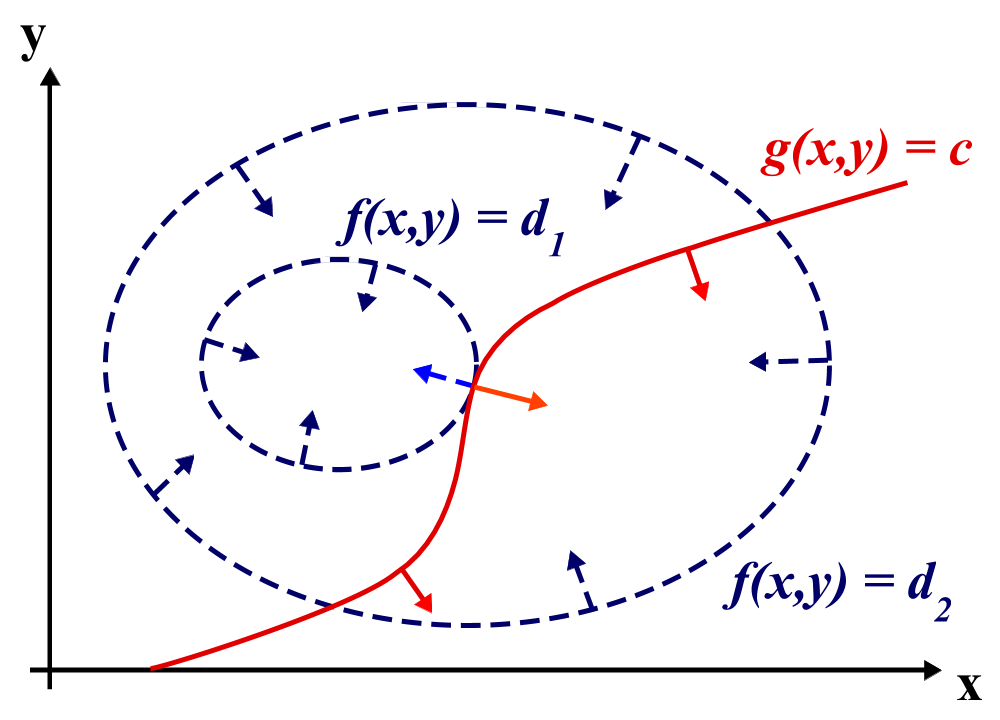
\includegraphics[width=0.5\linewidth]{lagrangian-optimization}
\end{center}
If the gradients were not parallel, we could move along $g(x,y)=c$ to a higher contour of $f(x,y)$ by following the component of $\nabla f$ parallel to $g(x,y)=c$.

	\chapter{Functional Derivatives}\label{app:functional-derivatives}

A functional is just a function of a function -- i.e.\ some rule $F$ that maps a function $f$ into a number $F[f]$.  Definite integrals are a common example.
In order to optimize a functional $F$ with respect to its argument $f$, one needs to take a \textit{functional derivative}.\footnote{\url{http://en.wikipedia.org/wiki/Functional_derivative}}
To motivate the definition of a functional derivative, first consider the definition of an ordinary derivative
\begin{align}
  \fd{f(x)}{x}
\equiv
  \lim_{\e\rightarrow0}
  \fr{f(x+\e)-f(x)}{\e}
\end{align}
and note the following identity, which you can verify using
$
  f(x+\e)
=
  f(x)
+
  \dfd{f(x)}{x}
  \e
+
  \mc{O}(\e^2)
$.
\begin{align}\label{eq:scalar-derivative-trick}
  \lim_{\e\rightarrow0}
  \fr{f(x+\e)-f(x)}{\e}
=&\
\left.
  \fr{df(x+\e)}{d\e}
\right|_{\e=0}
\end{align}
For multivariate functions, we have the concept of a \textit{directional derivative}
\begin{align}\label{eq:directional-derivative}
  \bo{y}\cdot
  \pd{f(\bo{x})}{\bo{x}}
=
  \lim_{\e\rightarrow0}
  \fr{f(\bo{x}+\e\bo{y}) - f(\bo{x})}{\e}
\end{align}
which measures the change in $f(\bo{x})$ in the direction $\bo{y}$.
Using equation \ref{eq:scalar-derivative-trick}, the directional derivative can be evaluated as an ordinary scalar derivative with respect to $\e$.
\begin{align}\label{eq:vector-derivative-trick}
  \bo{y}\cdot
  \pd{f(\bo{x})}{\bo{x}}
=
  \left.
  \fd{f(\bo{x} + \e\bo{y})}{\e}
  \right|_{\e=0}
\end{align}
The functional derivative $\dfr{\d F}{\d f}$ is defined to satisfy an equation analogous to \ref{eq:directional-derivative}, playing the role of the gradient.
\begin{align}
  \int_{-\infty}^{\infty}
  dx'\,
  g(x')
  \fr{\d F[f]}{\d f(x')}
\equiv
  \lim_{\e\rightarrow0}
  \fr{F[f+\e g] - F[f]}{\e}
\end{align}
This left-hand side could be called a \textit{functional directional derivative}, giving the change in $F$ upon displacing its argument along the function $g$.
Here, the integral takes the role of the dot product in \ref{eq:directional-derivative}.
Using the same trick as in equation \ref{eq:vector-derivative-trick}, the functional derivative can be expressed as an ordinary scalar derivative.
\begin{align}
\label{eq:functional-derivative-trick}
  \int_{-\infty}^{\infty}
  dx'\,
  g(x')
  \fr{\d F[f]}{\d f(x')}
=
  \left.
  \fd{F[f+\e g]}{\e}
  \right|_{\e=0}
\end{align}
The standard procedure for evaluating the functional derivative is to first evaluate the right-hand side of equation~\ref{eq:functional-derivative-trick} for an arbitrary $g$ and then infer what $\dfr{\d F[f]}{\d f(x)}$ must be by comparing to the left-hand side.
Equivalently, $g(x')$ can be replaced with a Dirac delta $\d(x-x')$ in order to arrive at $\dfr{\d F[f]}{\d f(x)}$ directly.

Using eq. \ref{eq:functional-derivative-trick} and the lemma in \cref{app:fundamental-lemma-of-calculus-of-variations}, we find that the stationarity condition for a functional
\begin{align}
  \fr{\d F[f]}{\d f}
\overset{!}{=}
  0
\end{align}
is equivalent to the following condition.
\begin{align}
  \left.
  \fd{F[f+\e g]}{\e}
  \right|_{\e=0}
\overset{!}{=}
  0
&&
  \text{for all $g(x)$}
\end{align}

	\chapter{Fundamental Lemma of Calculus of Variations}\label{app:fundamental-lemma-of-calculus-of-variations}

The \textit{Fundamental Lemma of Calculus of Variations}\footnote{\url{http://en.wikipedia.org/wiki/Fundamental_lemma_of_calculus_of_variations}} says that, for continuous functions, the condition
\begin{align}
  \int_{-\infty}^\infty dx f(x)\eta(x)
=
  0
\text{ for all $\eta(x)$}
\end{align}
holds only when $f(x)=0$ for all $x$.
We can see this by considering the case $\eta(x)=f(x)$.
Since $f(x)^2$ is nonnegative everywhere, the integral yields a positive number whenever $f(x)\neq 0$ on a finite range of $x$ values.

	\chapter{Unitary Invariances for Hartree-Fock Orbitals}\label{app:hartree-fock-orbital-invariance}


\paragraph{Orthonormality.}
By definition, unitary transformations preserve overlaps.
This can be verified as follows
\begin{align*}
  \ip{\tl\y_i|\tl\y_j}
=
\sum_{kl}
  U_{ki}U_{lj}^*
  \ip{\y_k|\y_l}
=
\sum_{kl}
  U_{ki}U_{lj}^*
  \delta_{kl}
=
\sum_k
  U_{ki}U_{kj}^*
=
  \delta_{ij}
\end{align*}
using $\sum_k U_{ki}U_{kj}^*=(\bo{U}\bo{U}\dg)_{ji}=(\bo{1})_{ji}=\d_{ji}$.

\paragraph{Fock operator.}
Only the Coulomb and exchange parts of the Fock operator depend on the orbital set.
For the Coulomb part, we have
{\small\begin{align*}
\sum_i
  \ip{\tl\y_i(2)|\op{g}(1,2)|\tl\y_i(2)}
=
\sum_{ijk}
  U_{ji}U_{ki}^*
  \ip{\y_j(2)|\op{g}(1,2)|\y_k(2)}
=
\sum_{jk}
  \delta_{jk}
  \ip{\y_j(2)|\op{g}(1,2)|\y_k(2)}
=
\sum_j
  \ip{\y_j(2)|\op{g}(1,2)|\y_j(2)}
\end{align*} \underline{}}%
using the fact that $\sum_i U_{ji}U_{ki}^*=\d_{jk}$.
For the exchange part, we have the same thing with a $\op{P}(1,2)$ sandwiched in there.

\paragraph{Hamiltonian expectation value.}
The vector notation $\bm\y$ for our orbitals allows us to express $\F$ and $\tl\F$ as
\begin{align*}
  \F(1,\ld,n)
=
  \tfrac{1}{\sqrt{n!}}
  |\bm\y(1)\cd\bm\y(n)|
%\sp\sp
  \tl\F(1,\ld,n)
=
  \tfrac{1}{\sqrt{n!}}
  |\tl{\bm\y}(1)\cd\tl{\bm\y}(n)|
\end{align*}
which, noting that the matrix $\ma{\tl{\bm\y}(1)\ \cd\ \tl{\bm\y}(n)}$ is simply
\begin{align*}
  \ma{\tl{\bm\y}(1)\ \cd\ \tl{\bm\y}(n)}
=
  \ma{\bo{U}\dg\bm\y(1)\ \cd\ \bo{U}\dg\bm\y(n)}
=
  \bo{U}\dg\ma{\bm\y(1)\ \cd\ \bm\y(n)}
\end{align*}
implies $\tl\F=\det(\bo{U}\dg)\F=\det(\bo{U})^*\F$.
Therefore, $\tl{\F}$ and $\F$ have the same energy expectation values.
\begin{align}
  \ip{\tl\F|\op{H}_e|\tl\F}
=
  \det(\bo{U}\bo{U}\dg)\ip{\F|\op{H}_e|\F}
=
  \ip{\F|\op{H}_e|\F}
\end{align}

	\chapter{The pull-through relation}\label{app:pull-through-relation}

\begin{prop}\label{prop:pull-through-relation}
\thmtitle{Pull-through relation}
\thmstatement{
  For any non-commuting $x_1,\ld,x_n$, and $y$ for which addition, subtraction and multiplication are defined, $x_1\cd x_ny=\pr{\mp}^nyx_1\cd x_n+\sum_{k=1}^n\pr{\mp}^{n-k}x_1\cd[x_k,y]_{\pm}\cd x_n$, where $[x,y]_{\pm}\equiv xy\pm yx$.
}
\thmproof{
  The $n=1$ case follows from the definition of the commutator brackets: $xy=\mp yx+[x,y]_{\pm}$.
  Now, assume it holds for $n$ and consider the $n+1$ case.
  Since $x_1\cd x_{n+1}y=x_1\cd x_n(\mp yx_{n+1}+[x_{n+1},y]_{\pm})$, we find
  \begin{align*}
    x_1\cd x_{n+1}y
  =&\
  \mp
    \pr{
      \pr{\mp}^nyx_1\cd x_n
    +
      \sum_{k=1}^n
      \pr{\mp}^{n-k}
      x_1\cd [x_k,y]_{\pm}\cd x_n
    }
    x_{n+1}
  +
    x_1\cd x_n[x_{n+1},y]_{\pm}
  \\=&\
    \pr{\mp}^{n+1}
    yx_1\cd x_{n+1}
  +
    \sum_{k=1}^{n+1}
    \pr{\mp}^{n+1-k}
    x_1\cd[x_k,y]_{\pm}\cd x_{n+1}
  \end{align*}
  and, by induction, the result holds for all $n$.
}
\end{prop}
\end{appendices}

%\backmatter
\printindex

\end{document}